
\documentclass[%
  aspectratio=169,
  9pt,
  USenglish,
  %titlegraphic, % store custom image to .images/titlegraphic
  %affiliationintitlepagehead,
  %progressbar,
%   affiliation,
]{beamer}
%\texttt{}

\usetheme{TUM}


\newcommand{\coorg}{Irisa}


\setbeamertemplate{blocks}[rounded][shadow=false]

\usepackage{tikz}  
\usepackage{tikz-3dplot} 
\usepackage{graphicx}
\usepackage{media9}
\usetikzlibrary{positioning}

\usepackage{amsmath}
\usepackage{booktabs}

% change the camera position
\tdplotsetmaincoords{45}{135}

\usepackage{tabularx}

\usepackage{subcaption}

\usepackage{animate}

\usepackage{pgfmath}
\newcommand\randmin{}
\newcommand\randmax{}
\newcommand\randmultof{}
\newcommand\setrand[4]%
{\def\randmin{#1}%
	\def\randmax{#2}%
	\def\randmultof{#3}%
	\pgfmathsetseed{#4}%
}
\newcommand\nextrand
{\pgfmathparse{int(int((rnd*(\randmax-\randmin+1)+\randmin)/\randmultof)*\randmultof)}%
	\xdef\thisrand{\pgfmathresult}%
}

%\usepackage[backend=biber]{biblatex}
%\addbibresource{bib/references.bib}

\newcommand{\wave}{
	\begin{tikzpicture}[xscale=.05,yscale=.2]
	\draw[-,fill=white] plot[domain=0:10*pi,smooth] (\x,{sin(\x r)});
	\end{tikzpicture}
}


\newcommand{\domain}[4]{
	%% spatial,spectral,temporal
	\draw[fill=#4, opacity=.2] (#1,0,0) -- (0,#2,0) -- (0,0,#3) -- (#1,0,0);
}


\newcommand{\radarwave}{
	\begin{tikzpicture}[xscale=.1,yscale=.2]
	\draw[-,fill=white] plot[domain=0:5*pi,smooth] (\x,{sin(\x r)});
	\end{tikzpicture}
}


\newcommand{\earth}{
	\begin{tikzpicture}[baseline=-.25em, inner sep=0]
	\node{\includegraphics[width=8mm]{images/icons/earth}};
	\end{tikzpicture}
}

\newcommand{\sat}{
	\begin{tikzpicture}[baseline=-.25em, inner sep=0]
	\node[rotate=270,anchor=center]{\includegraphics[width=8mm]{images/icons/sat2}};
	\end{tikzpicture}
}


\usepackage[capitalize]{cleveref}
\usepackage[square,sort,comma,numbers]{natbib}

%% this hack seems to be nececessary due to incompatibilities of cvpr template and tikz... -> https://tex.stackexchange.com/questions/398223/tikz-gives-error-command-everyshipouthook-already-defined
%\makeatletter
%\@namedef{ver@everyshi.sty}{}
%\makeatother
%% hackend

\usepackage{tikz}
\usepackage{pgfplots}
\usetikzlibrary{positioning, calc,arrows,arrows.meta, fit}
%\usetikzlibrary{arrows.meta,calc,decorations.markings,math,arrows.meta}
\usepgfplotslibrary{groupplots}
\usepgfplotslibrary{fillbetween}
\usepgfplotslibrary{statistics} % provides boxplots
\usepackage{xfrac}

\newcommand{\tp}{tp}
\newcommand{\tn}{tn}
\newcommand{\fp}{fp}
\newcommand{\fn}{fn}


\usepackage{tumcolors}
\usepackage{tummath}
\newcommand{\yhat}{\hat{\V{y}}}
\newcommand{\ycorrect}{\hat{y}^+}
\newcommand{\thetadelta}{\V{\Theta}_\delta}
\newcommand{\biasdelta}{b_\delta}
\newcommand{\biasclass}{\V{b}_\text{c}}
\newcommand{\thetaclass}{\V{\Theta}_\text{c}}
\newcommand{\thetafeat}{\V{\Theta}_\text{feat}}
\newcommand{\fclass}{f_\text{c}}
\newcommand{\fdelta}{f_\delta}
\newcommand{\ffeat}{f_\text{feat}}
\newcommand{\f}{f}

\newcommand{\rvtime}{T_c} 
\newcommand{\xuptot}{\M{X}_{\rightarrow t}} 
\newcommand{\deltauptot}{\delta_{\rightarrow t}} 
\newcommand{\tstop}{\ensuremath{t_\text{stop}}}
\newcommand{\meantstop}{\ensuremath{\bar{t}_\text{stop}}}
\usepackage[super]{nth}
\usepackage{mathtools}

\definecolor{evalcolor}{HTML}{3F3F3F}
\definecolor{traincolor}{HTML}{B98951}
\definecolor{validcolor}{HTML}{3F4BBE}

\definecolor{fdlcolor}{HTML}{142737}

\usepackage{multimedia}

\colorlet{colortrain}{tumblue}
\colorlet{colorinfer}{tumblack}

\colorlet{earlinesscolor}{tumblue}
\colorlet{accuracycolor}{tumorange}

\colorlet{stdcolor}{tumbluelight}
\colorlet{mediancolor}{tumorange}
\colorlet{meancolor}{tumblue}

\colorlet{b1color}{tumdiagramaubergine}
\colorlet{b2color}{tumdiagramnavyblue}
\colorlet{b3color}{tumdiagramturquoise}
\colorlet{b4color}{tumdiagramgreen}
\colorlet{b5color}{tumdiagramlimegreen}
\colorlet{b6color}{tumdiagramyellow}
\colorlet{b7color}{tumdiagramsand}
\colorlet{b8color}{tumdiagramredorange}
\colorlet{b8Acolor}{tumdiagramred}
\colorlet{b9color}{tumblack}
\colorlet{b10color}{tumblue}
\colorlet{b11color}{tumdiagramdarkred}
\colorlet{b12color}{tumorange}

% atmospheric bands
\colorlet{b1color}{tumblack}%tumdiagramaubergine
\colorlet{b9color}{tumblack}%tumblack
\colorlet{b10color}{tumblack}%tumblue

%visisble bands
\colorlet{b2color}{tumblue}%tumdiagramnavyblue
\colorlet{b3color}{tumblue}%tumdiagramturquoise
\colorlet{b4color}{tumblue}%tumdiagramgreen

% near infrared bands
\colorlet{b5color}{tumdiagramred}%tumdiagramlimegreen
\colorlet{b6color}{tumdiagramred}%tumdiagramyellow
\colorlet{b7color}{tumdiagramred}%tumdiagramsand
\colorlet{b8color}{tumdiagramred}%tumdiagramredorange
\colorlet{b8Acolor}{tumdiagramred}%tumdiagramred

% SWIR bands
\colorlet{b11color}{tumorange}%tumdiagramdarkred
\colorlet{b12color}{tumorange}%tumorange

\colorlet{epsilon0color}{tumorange}
\colorlet{epsilon1color}{tumblue}
\colorlet{epsilon10color}{tumblack}

\colorlet{gridcolor}{tumblue}
\colorlet{activationcolor}{tumorange}

\colorlet{meadowcolor}{tumbluemedium}
\colorlet{wbarleycolor}{tumbluedark}
\colorlet{corncolor}{tumorange}
\colorlet{wheatcolor}{tumgreen}
\colorlet{sbarleycolor}{tumdiagramred}
\colorlet{clovercolor}{tumdiagramturquoise}
\colorlet{triticalecolor}{tumdiagramsand}

\tikzstyle{rnn}=[draw,circle, inner sep=.1em]
\tikzstyle{norm}=[rounded corners,draw]
\tikzstyle{annot}=[rounded corners, fill=tumblue!20]
\tikzstyle{infer}=[-stealth, shorten >=.0em, shorten <=.0em, colorinfer]
\tikzstyle{loss}=[fill=tumblue!10, rounded corners, font=\small]
\tikzstyle{grad}=[colortrain]

\newcommand{\ptoffset}{\varepsilon}

\tikzstyle{test} = [thick]
\tikzstyle{train} = [thin, dotted]

\usepackage[inline]{enumitem}
\setenumerate{label=(\roman*),itemsep=3pt,topsep=3pt}

\setlength{\belowcaptionskip}{-10pt}


\colorlet{traincolor}{tumbluelight}
\colorlet{validcolor}{tumbluedark}
\colorlet{evalcolor}{tumorange}

\colorlet{forwardcolor}{tumblue}
\colorlet{backwardcolor}{tumorange}

% defaultvalue -> might be replaced later
\colorlet{tensorcolor}{forwardcolor}

\colorlet{classcolor}{tumivory}
\colorlet{encodercolor}{tumblue}
\colorlet{encodercolor}{tumblue}
\colorlet{colorblue}{tumblue}
\colorlet{colororange}{tumorange}

\colorlet{colorclassone}{tumblue}
\colorlet{colorclasstwo}{tumblack}
\colorlet{colorclassthree}{tumorange}
\colorlet{colorclassfour}{tumgray}

\colorlet{frh01color}{tumgray}
\colorlet{frh02color}{tumorange}
\colorlet{frh03color}{tumblue}
\colorlet{frh04color}{tumblack}



%\usepackage{media9}

% notation
\newcommand{\MWeight}{\ensuremath{\M{W}}}
\newcommand{\VBias}{\ensuremath{\V{b}}}
\newcommand{\VInput}{\DataVec}
\newcommand{\VHidden}{\ensuremath{\V{h}}}
\newcommand{\FActivation}{\ensuremath{\sigma}}
\newcommand{\VCellState}{\ensuremath{\V{c}}}
\newcommand{\VForgetGate}{\ensuremath{\V{f}}}
\newcommand{\VModulationGate}{\ensuremath{\V{j}}}
\newcommand{\VInputGate}{\ensuremath{\V{i}}}
\newcommand{\VOutputGate}{\ensuremath{\V{o}}}
\newcommand{\concat}[2]{\left[#1 \parallel #2\right]}


\newcommand{\VResetGate}{\ensuremath{\V{r}}}
\newcommand{\VUpdateGate}{\ensuremath{\V{u}}}


%\usepackage{titlesec}
%\titlespacing{\section}{0pt}{10pt}{3pt}


\usetikzlibrary{3d}
\tikzstyle{perspective3d}=[
x={(0.5cm,0.5cm)}, y={(1cm,0cm)}, z={(0cm,1cm)}]


\usetikzlibrary{spy}

\usetikzlibrary{external,pgfplots.dateplot}

\usepackage[eulergreek]{sansmath}
\pgfplotsset{
	y tick label style={/pgf/number format/.cd,%
		scaled y ticks = false,
		set thousands separator={},
		fixed},
	x tick label style={/pgf/number format/.cd,%
		scaled x ticks = false,
		set decimal separator={,},
		fixed},
	tick label style = {font=\scriptsize\sansmath\sffamily},
	every axis label = {
		font=\scriptsize\sansmath\sffamily},
	every axis/.append style={
		axis lines=left, 
		enlargelimits, 
		thick},
	legend style = {font=\scriptsize\sansmath\sffamily, draw=none, rounded corners=0, fill opacity=.5, text opacity=1},
	label style = {font=\scriptsize\sansmath\sffamily},
	grid style={line width=.1pt, draw=gray!10},
	major grid style={line width=.2pt,draw=tumgraylight},
}

%\let\tempone\itemize
%\let\temptwo\enditemize
%\renewenvironment{itemize}{\tempone\addtolength{\itemsep}{-.5\baselineskip}}{\temptwo}

\tikzstyle{circ} = [circle, draw=white, fill=tumblue, inner sep=1pt]
\newcommand{\fcn}{
	\begin{tikzpicture}[scale=0.2, rotate=0, baseline=-.25em, inner sep=1pt]
	\node[circ](a0) at (0,-1){};
	\node[circ](a1) at (0,0){};
	\node[circ](a2) at (0,1){};
	
	\node[circ](b0) at (1,-0.5){};
	\node[circ](b1) at (1,0.5){};
	
	\draw[-] (a0) -- (b0);
	\draw[-] (a1) -- (b0);
	\draw[-] (a2) -- (b0);
	
	\draw[-] (a0) -- (b1);
	\draw[-] (a1) -- (b1);
	\draw[-] (a2) -- (b1);
	
	\end{tikzpicture}
}

\newcommand{\lfcn}[1]{
	\begin{tikzpicture}[scale=#1, rotate=0, baseline=-.25em, inner sep=1pt]
	\node[circle, draw=white, fill=tumblue, inner sep=3](a0) at (0,-1){};
	\node[circle, draw=white, fill=tumblue,  inner sep=3](a1) at (0,0){};
	\node[circle, draw=white, fill=tumblue,  inner sep=3](a2) at (0,1){};
	
	\node[circle, draw=white, fill=tumblue,  inner sep=3](b0) at (1,-0.5){};
	\node[circle, draw=white, fill=tumblue,  inner sep=3](b1) at (1,0.5){};
	
	\draw[-] (a0) -- (b0);
	\draw[-] (a1) -- (b0);
	\draw[-] (a2) -- (b0);
	
	\draw[-] (a0) -- (b1);
	\draw[-] (a1) -- (b1);
	\draw[-] (a2) -- (b1);
	
	\end{tikzpicture}
}

\newcommand{\hidden}[1]{
	\begin{tikzpicture}[scale=.1, baseline=-.25em]	
	%\draw[step=1.0,black,thin] (0,0) grid (#1,1);
	\foreach \i in {1,...,#1}{
		\node[circle, draw=white, fill=tumbluelight, inner sep=1pt] at (\i,0){};
	}
	\end{tikzpicture}
}

\newcommand{\drawvector}[1]{
	\begin{tikzpicture}[scale=.1, baseline=-.25em]	
	%\draw[step=1.0,black,thin] (0,0) grid (#1,1);
	\foreach \i in {1,...,#1}{
		\node[circ] at (\i,0){};
	}
	\end{tikzpicture}
}

\title{Early Classification for Agricultural Monitoring}
\subtitle{from Satellite Time Series}
\author[M. Rußwurm, R. Tavenard, S. Lefèvre, M.Körner]{Marc Rußwurm, Romain Tavenard, Sébastien Lefèvre, Marco Körner}
\institute[TUM, IRISA-Obelix, LETG-Rennes]{Technical University of Munich, Germany\\
                Remote Sensing Technology}
\date{\today}

\begin{document}
\begin{frame}[t]
  \titlepage
\end{frame}

%{\setbeamercolor{background canvas}{bg=tumbluedark}
%	\begin{frame}[plain]
%		
%		\vfill
%		\Huge\color{white}
%		\begin{center}
%			\begin{columns}
%				\column{.5\textwidth}
%				\vspace{7em}
%				
%				\hfill 
%				Vegetation and Agriculture
%				\column{.5\textwidth}
%				
%				%\includegraphics[width=7cm]{images/fdl}
%			\end{columns}
%		\end{center}
%		
%		\vfill
%	\end{frame}
%}

%\begin{frame}
%	\frametitle{Power Plants}
%	\begin{tikzpicture}
%		\node(a){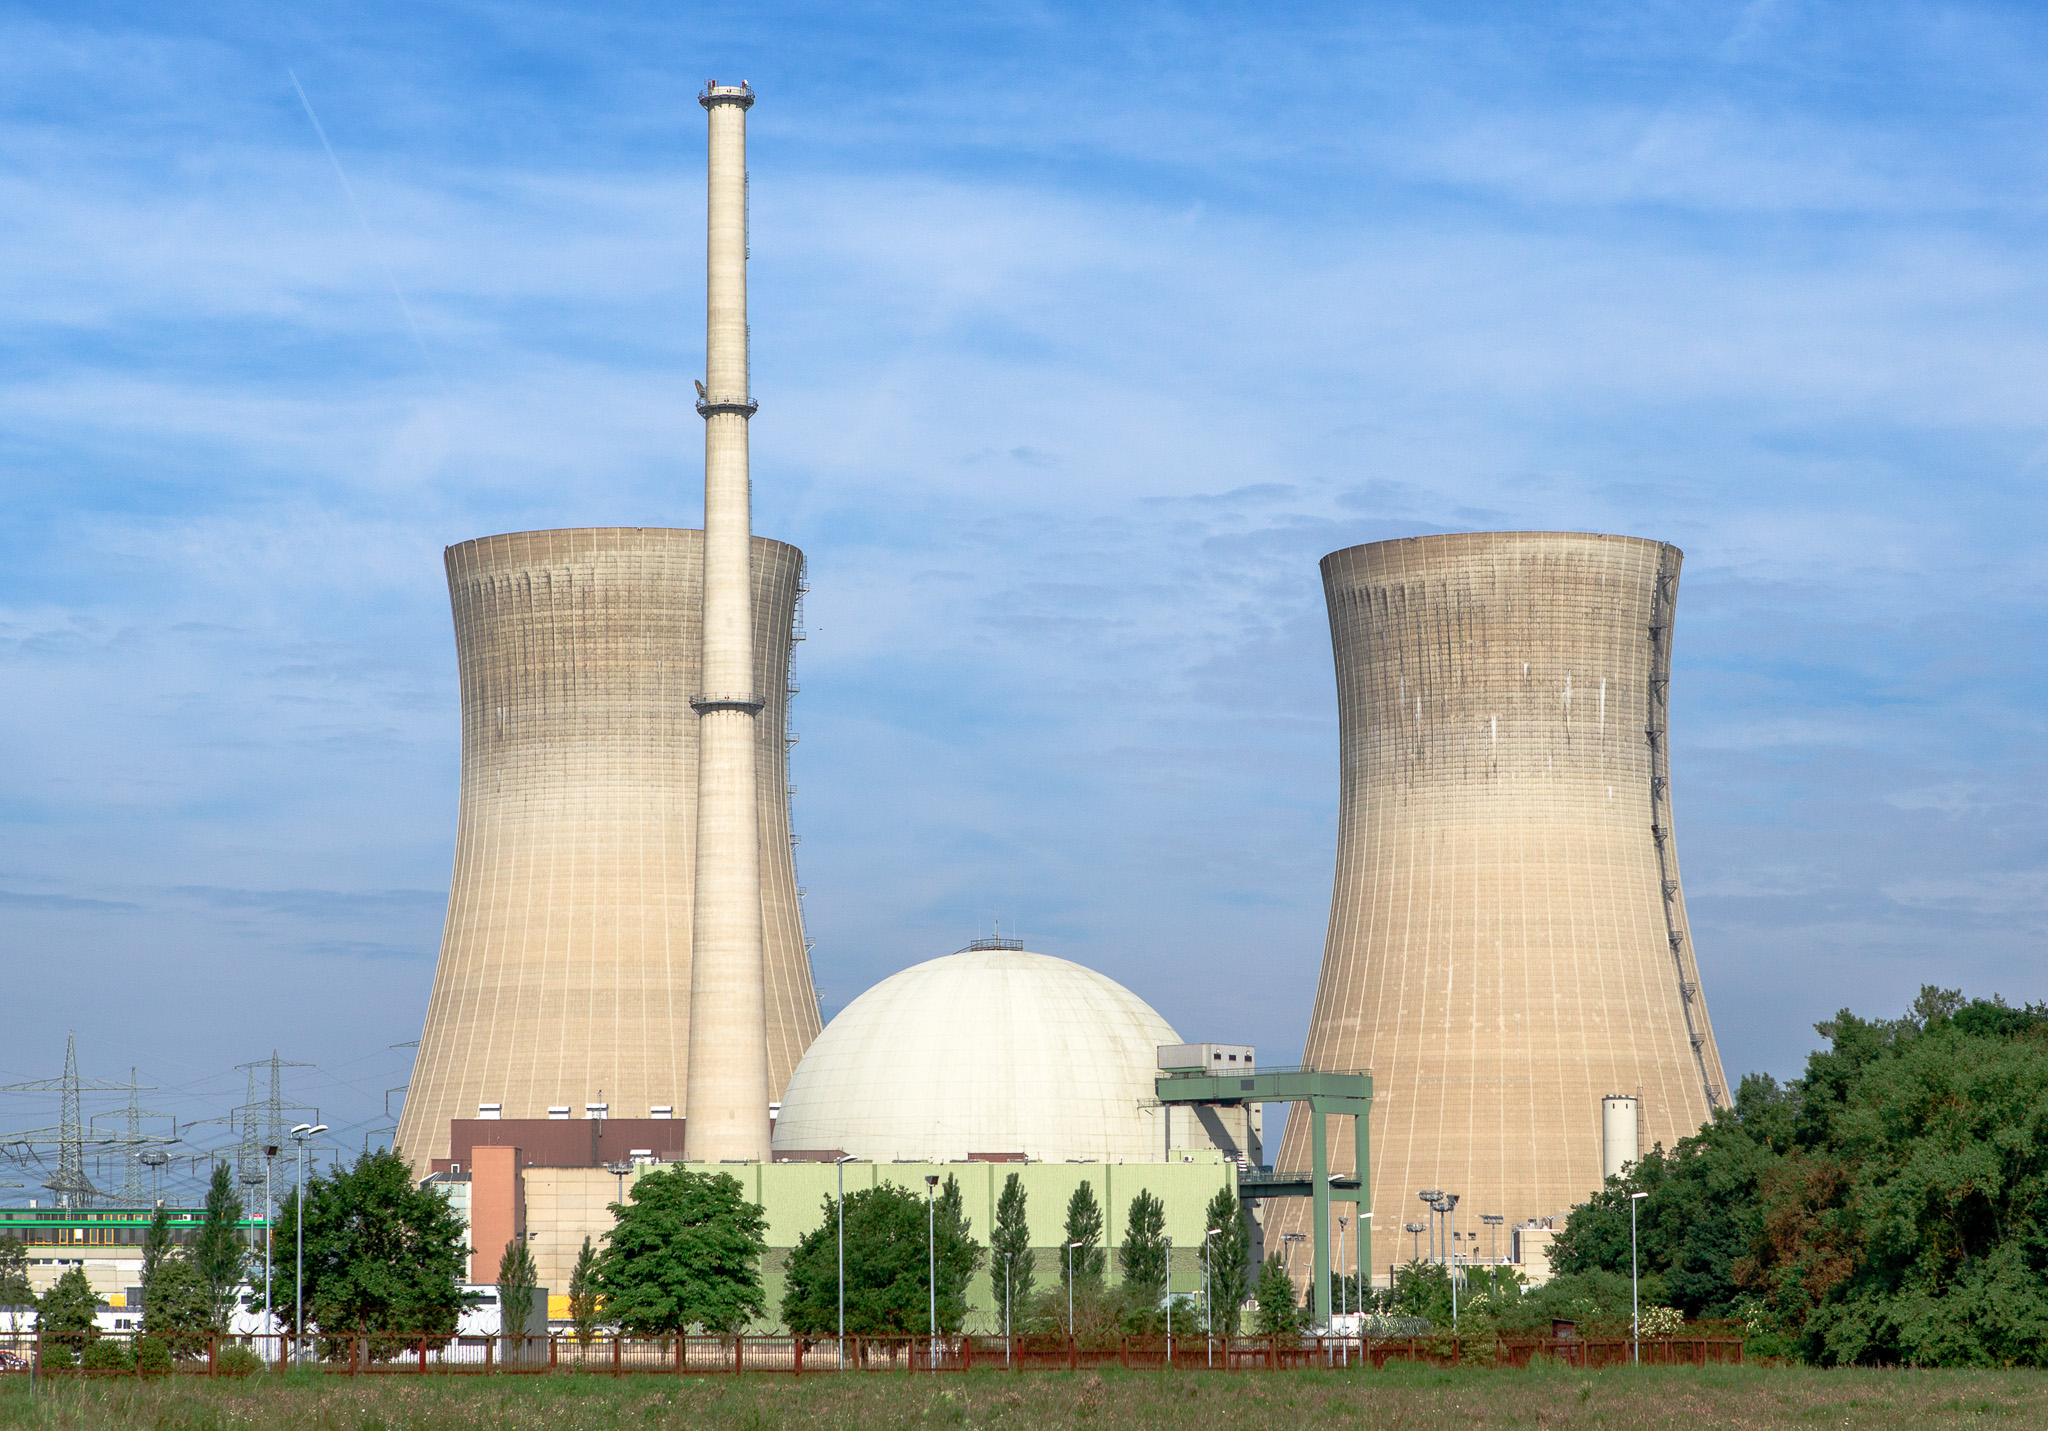
\includegraphics[height=3cm]{images/powerplants/akw.jpg}};
%		\node[right=of a](b){\includegraphics[height=3cm]{images/powerplants/windrad.jpg}};
%		\node[right=of b](b){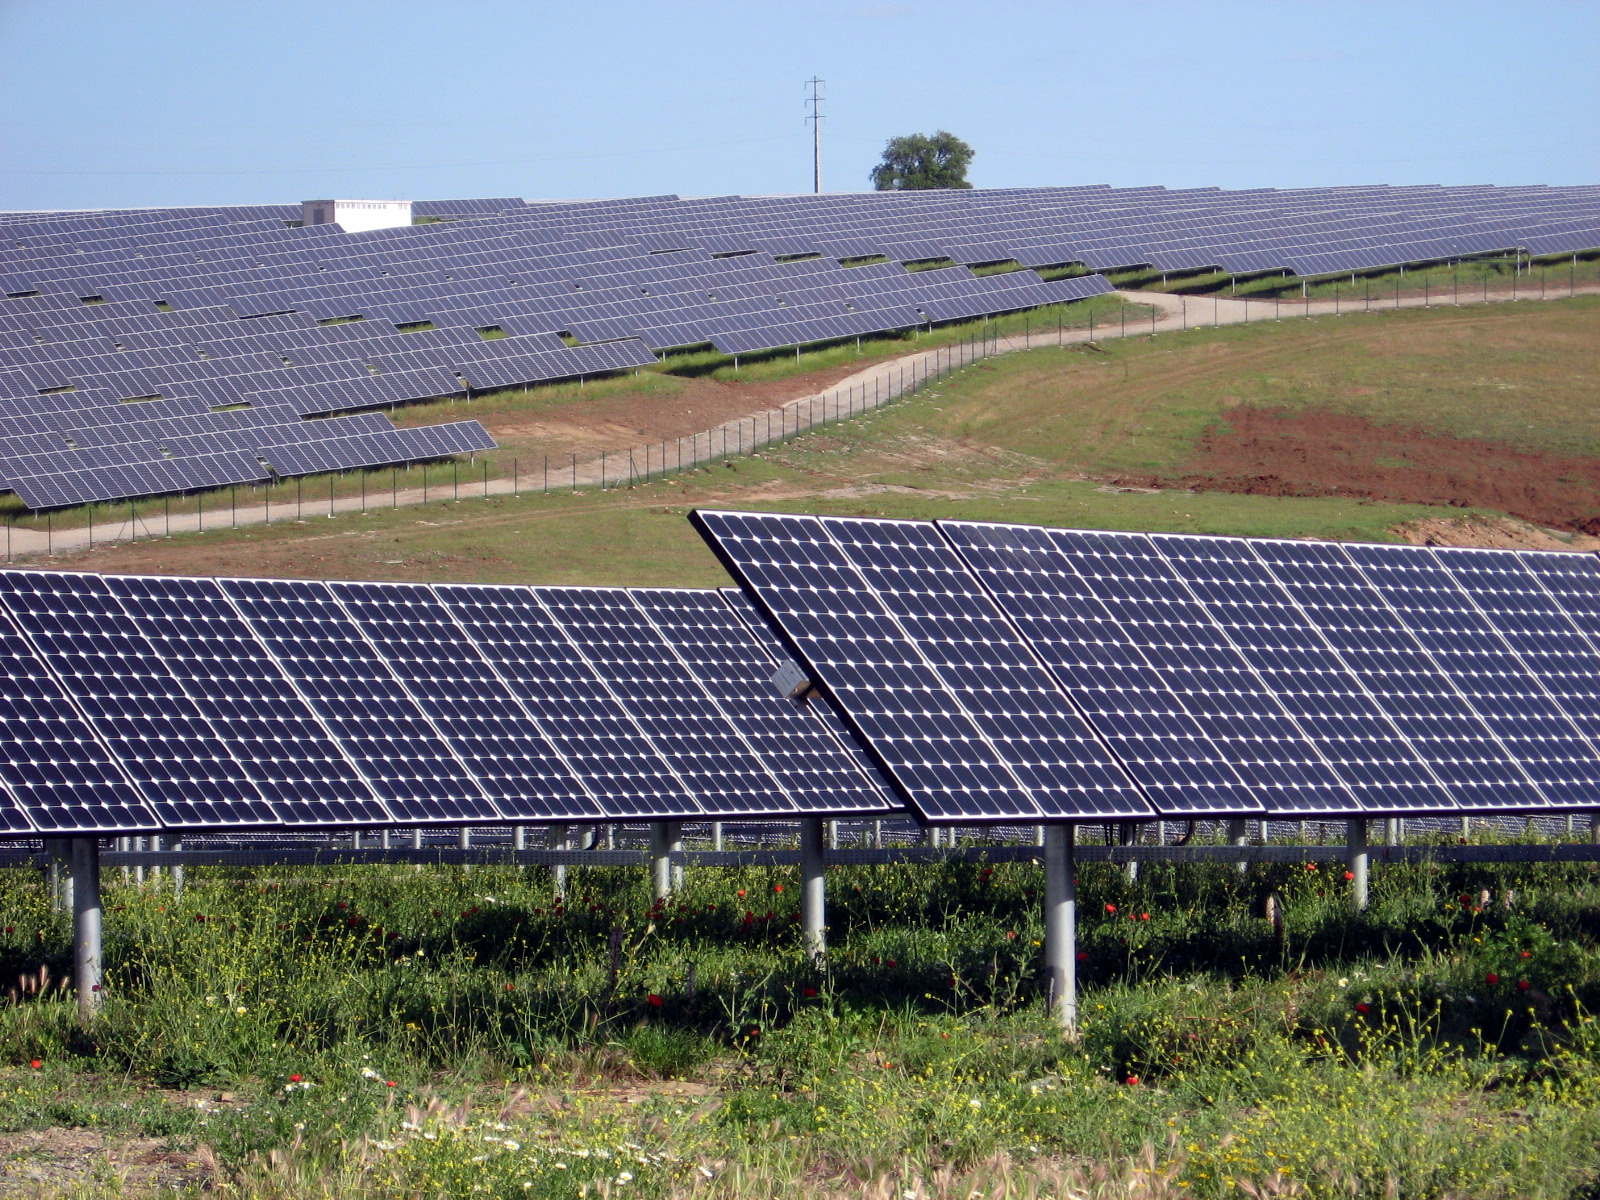
\includegraphics[height=3cm]{images/powerplants/solar.jpg}};
%	\end{tikzpicture}
%	
%\end{frame}
%
%
\begin{frame}
	\frametitle{Photosynthesis: Light $\rightarrow$ Life}
	\framesubtitle{Vegetation}
	
	\begin{columns}[b]
		\column{.5\textwidth}
		Spectral characteristics
		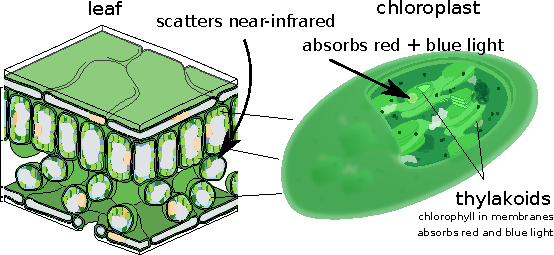
\includegraphics[width=\textwidth]{images/leaf_smallannot.pdf}
		common remote sensing feature: $\text{NDVI} = \frac{\text{NIR} - \text{RED}}{\text{NIR} + \text{RED}}$ \\
		{\scriptsize images modified from wikipedia cc}
		\column{.5\textwidth}
		Temporal characteristics
		\includemedia[
		width=\textwidth,
		activate=pageopen,
		addresource=mp4/apenne_modis_ndvi.mp4,
		flashvars={source=mp4/apenne_modis_ndvi.mp4&loop=true&
			autoPlay=true}
		]{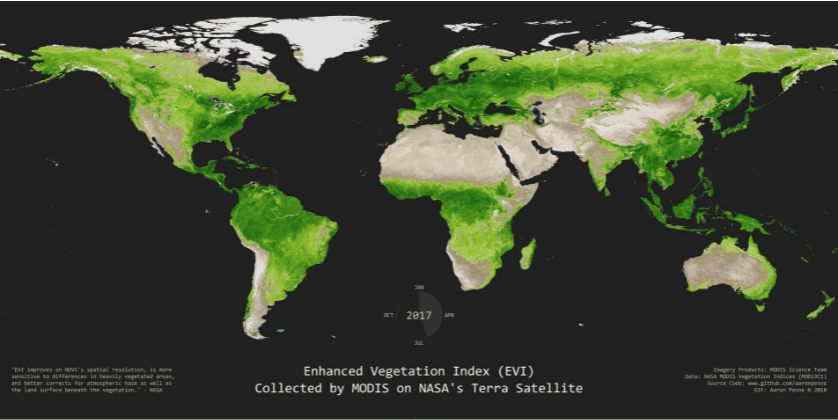
\includegraphics[width=\textwidth]{mp4/apenne_modis_ndvi.png}}{mp4/apenne_modis_ndvi.mp4}
		{\scriptsize visualization \href{https://github.com/aaronpenne}{Aaron Penne Github}}
		
	\end{columns}
	
	\vspace{2em}
	Vegetation follows \textbf{seasonal life cycles} (phenology) which can be used to \textbf{distinguish categories}. 
	
\end{frame}

\begin{frame}
	\frametitle{Why do we want to classify vegetation?}
	\framesubtitle{Distinguishing Vegetation}
	\begin{columns}
		\column{.5\textwidth}
		\begin{description}
			\item[Food security] Estimate the expected yield (from cultivated area) to predict food prices, shortages in countries that collect few agronomic statistics.
			\pause
			\item[Precision Agriculture] Identifying vegetation is a first step to provide personalized recommendations to farmers on machining practices and location-based fertilizer use.
			\pause
			\item[Subsidy control] In Europe: monitor and control crop subsidy payments for European farmers.
			%				\item Precision agriculture: sd
		\end{description}
		\column{.5\textwidth}
		
\includegraphics[width=\textwidth]{images/sdg_goals.pdf}
	\end{columns}
	
\end{frame}

{\setbeamercolor{background canvas}{bg=tumbluedark}
	\begin{frame}[plain]
		
		\vfill
		\Huge\color{white}
		\begin{center}
			\begin{columns}
				\column{.5\textwidth}
				\vspace{7em}
				
				\hfill 
				Earth Observation
				\column{.5\textwidth}
				
				%\includegraphics[width=7cm]{images/fdl}
			\end{columns}
		\end{center}
		
		\vfill
	\end{frame}
}

\begin{frame}
	\frametitle{Earth Observation}
	\framesubtitle{Satellite Data}
	\begin{columns}
		\column{.5\textwidth}
			\vspace{-1em}
			\begin{tikzpicture}
	\node[label={above=0em:\scriptsize growth stages of corn Mimić et al., 2020}, inner sep=0](a){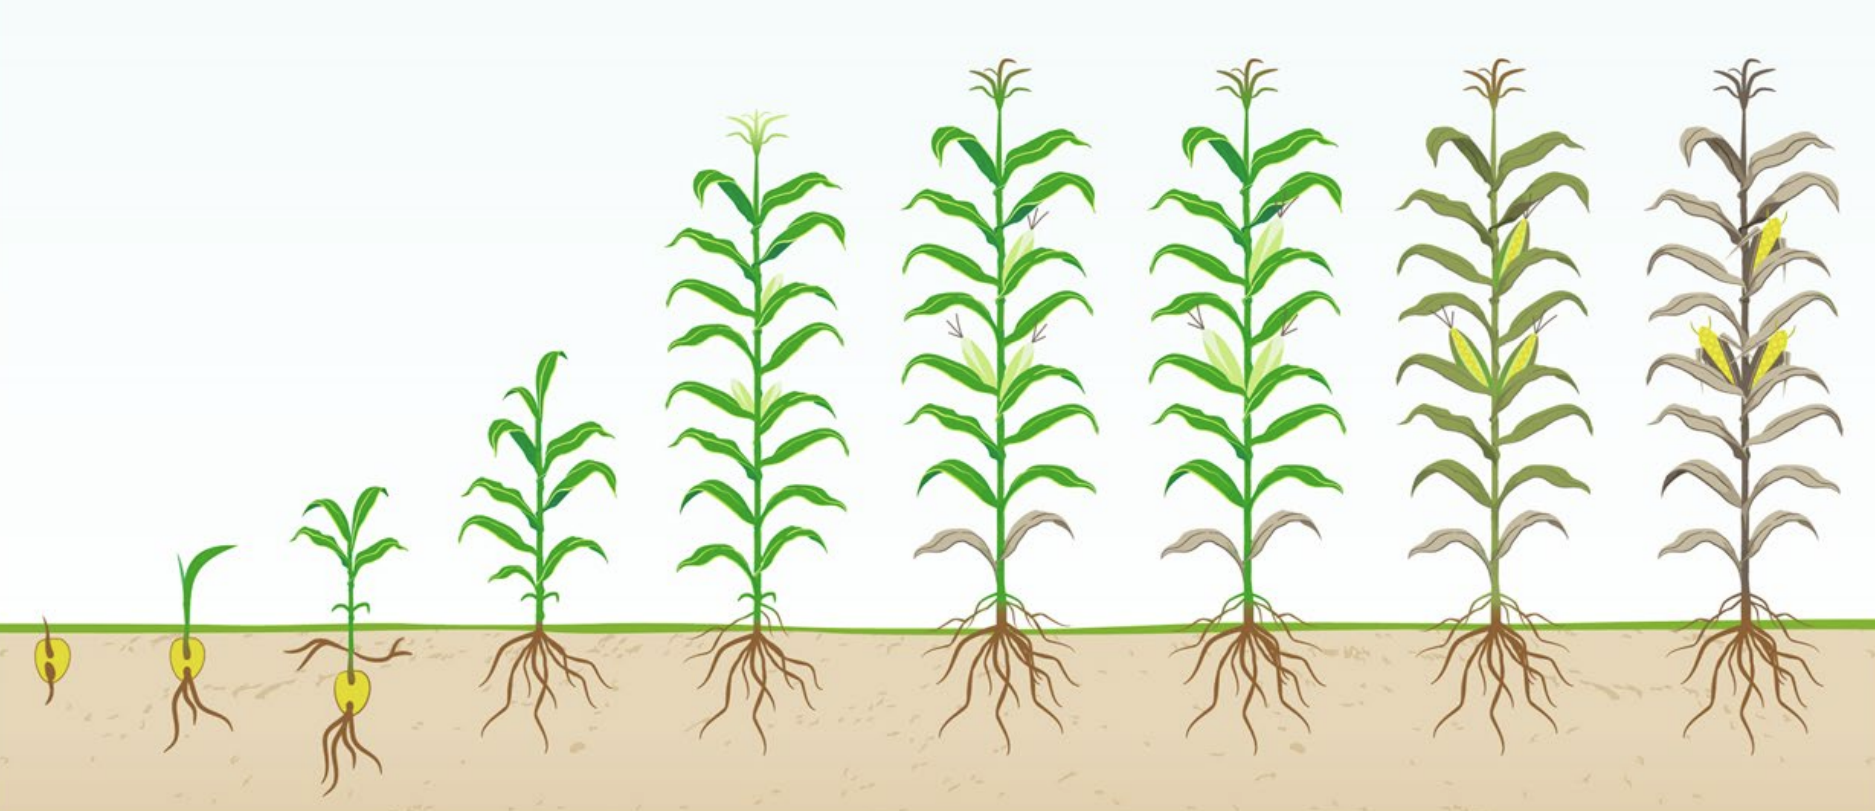
\includegraphics[width=6cm]{images/mimicetal2020_phenology_maize_.png}};
	
	\node[below=-1em of a] (b){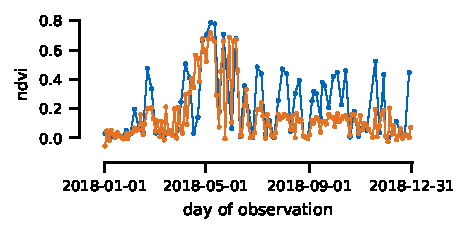
\includegraphics{images/ndvi}};
	
	\coordinate(left)  at ($(a.south west)+(-4.3em,0)$);
	\coordinate(right) at ($(a.south east)+(1.1em,0)$);
	
	\coordinate(veannot) at ($(left)!0.22!(right)$){};
	\coordinate(vtwoannot) at ($(left)!0.275!(right)$){};
	\coordinate(vfiveannot) at ($(left)!0.34!(right)$){};
	\coordinate(vtenannot) at ($(left)!0.42!(right)$){};
	\coordinate(btnnot) at ($(left)!0.5!(right)$){};
	\coordinate(rtwoannot) at ($(left)!0.6!(right)$){};
	\coordinate(rthreeannot) at ($(left)!0.7!(right)$){};
	\coordinate(rfiveannot) at ($(left)!0.8!(right)$){};
	\coordinate(harvestannot) at ($(left)!0.9!(right)$){};
	
	\coordinate(ve) at      ($ (b.center)+(-4em  ,1em) $);
	\coordinate(vtwo) at    ($ (b.center)+(-3em  ,1em) $);
	\coordinate(vfive) at   ($ (b.center)+(-2.5em,3em) $);
	\coordinate(vten) at    ($ (b.center)+(-2em  ,4em) $);
	\coordinate(bt) at      ($ (b.center)+(-1.5em,4.5em) $);
	\coordinate(rtwo) at    ($ (b.center)+(-1em  ,4.5em) $);
	\coordinate(rthree) at  ($ (b.center)+(-0em  ,2em) $);
	\coordinate(rfive) at   ($ (b.center)+(1.5em ,0.5em) $);
	\coordinate(harvest) at ($ (b.center)+(3em   ,0.5em) $);
	
	\draw[o-,tumorange](veannot)      -- (ve);
	\draw[o-,tumorange](vtwoannot)    -- (vtwo);
	\draw[o-,tumorange](vfiveannot)   -- (vfive);
	\draw[o-,tumorange](vtenannot)    -- (vten);
	\draw[o-,tumorange](btnnot)       -- (bt);
	\draw[o-,tumorange](rtwoannot)    -- (rtwo);
	\draw[o-,tumorange](rthreeannot)  -- (rthree);
	\draw[o-,tumorange](rfiveannot)   -- (rfive);
	\draw[o-,tumorange](harvestannot) -- (harvest);
	\end{tikzpicture}
			
			{\tiny Mimić, G., Brdar, S., Brkić, M., Panić, M., Marko, O., \& Crnojević, V. (2020). engineering Meteorological features to Select Stress tolerant Hybrids in Maize. Scientific reports, 10(1), 1-10.}
		\column{.5\textwidth}
			Sentinel 2. {\small every 2-5 days at $10m\times10m$ resolution}.
			\includemedia[
			width=\textwidth,
			activate=pageopen,
			addresource=mp4/sentinel2.mp4,
			flashvars={source=mp4/sentinel2.mp4&loop=true&
				autoPlay=true}
			]{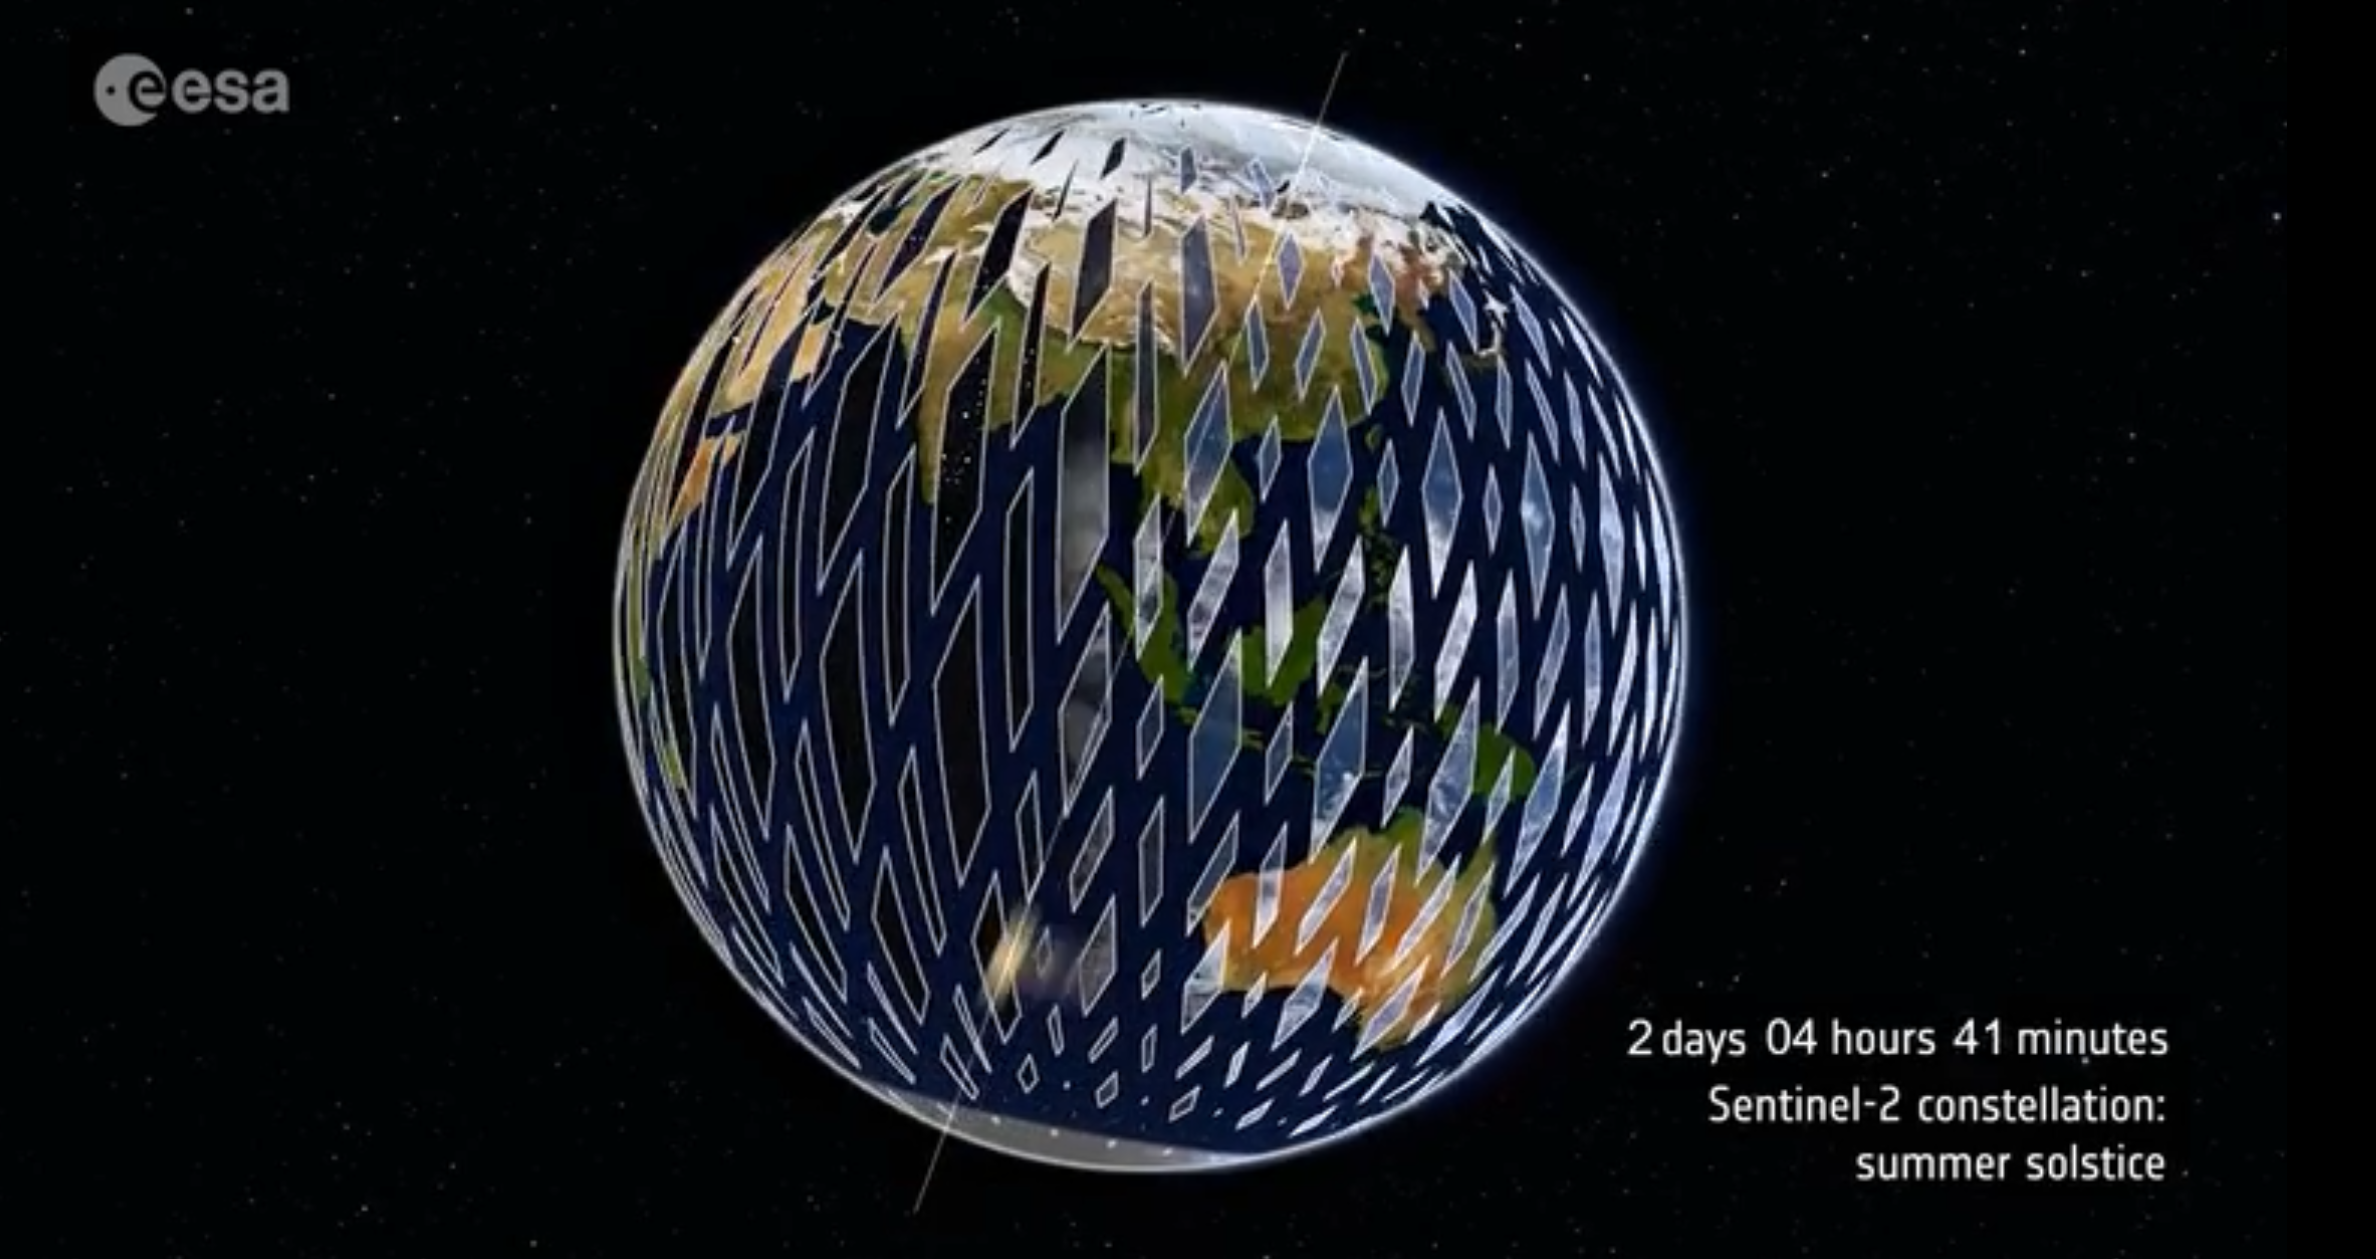
\includegraphics[width=\textwidth]{mp4/sentinel2.png}}{mp4/sentinel2.mp4}
			Source \href{https://www.esa.int/ESA_Multimedia/Videos/2016/08/Sentinel-2_global_coverage}{ESA}
	\end{columns}
\end{frame}

\begin{frame}
	\frametitle{Classifying Vegetation}
	\begin{columns}[t]
		\column{.5\textwidth}
			\hspace{1em} with hand-defined features
			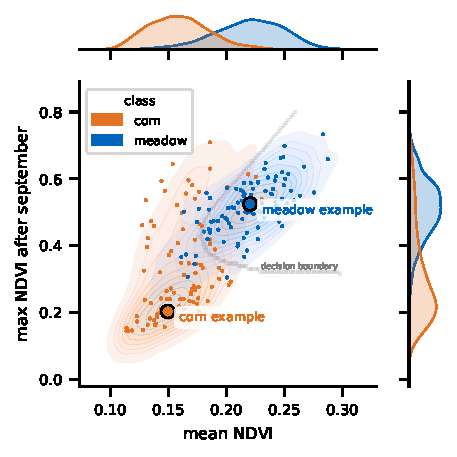
\includegraphics[width=6cm]{images/jointplot}
		\only<1->{
		\column{.5\textwidth}
			features learned from data
			\vspace{2em}
			\tikzstyle{annotation} = [font=\small, text width=3.5cm]
			\tikzstyle{node} = [circle, draw, font=\small]
			\tikzstyle{edge} = [-stealth, tumgray]
			\tikzstyle{operation} = [font=\scriptsize, fill=white, text=black]
			\tikzstyle{normal} = [font=\scriptsize, text=tumblue]
			\begin{tikzpicture}[node distance=0, xscale=2]
			
			
			
%			\node(a){\includegraphics[width=3cm]{nn/x.pdf}};
%			\node[right=of a](b){\includegraphics[width=4.5cm]{nn/h.pdf}};
%			\node[right=of b](c){\includegraphics[width=4.5cm]{nn/h2.pdf}};
%			\node[right=1em of c](d){\includegraphics[width=1.2cm]{nn/y.pdf}};
			
%			\coordinate(annotations) at (0,-3);
%			\node[annotation] at (a |- annotations){(a) Input space \\ $\mathbf{x} = (x_1, x_2)$};
%			\node[annotation] at (b |- annotations){(b) linear projection $\mathbf{w}_1^T\mathbf{x}$ into $\mathbb{R}^3$};
%			\node[annotation, xshift=-2em] at (c |- annotations){(c) non-linear distortion with $\tanh(\mathbf{w}_1^T\mathbf{x})$};
%			\node[annotation] at (d |- annotations){(d) Output class probabilities $y \in [0,1]$};
			
			\coordinate(network) at (0,3);
			\coordinate(networklone) at (1,3);
			\coordinate(networkltwo) at (2,3);
			\coordinate(networklthree) at (3,3);
			\coordinate(networklast) at (4,3);
			
			\node[node, above=of networklone](xone){$x_1$};
			\node[node, below=of networklone](xtwo){$x_2$};
			\begin{scope}[node distance=1.3em]
			\node[node, above=of networkltwo](hone){$h_1$};
			\node[node] at (networkltwo)(htwo){$h_2$};
			\node[node, below=of networkltwo](hthree){$h_3$};
			\end{scope}
			
			\begin{scope}[node distance=1.3em]
			\node[node, above=of networklthree](hhone){$\hat{h}_1$};
			\node[node] at (networklthree)(hhtwo){$\hat{h}_2$};
			\node[node, below=of networklthree](hhthree){$\hat{h}_3$};
			\end{scope}
			
			%			\node[node] at (networklthree){a};
			\node[node](y) at (networklast){$y$};
			
			\draw[edge] (xone) -- (hone);
			\draw[edge] (xone) -- (htwo);
			\draw[edge] (xone) -- (hthree);
			\node[operation] at ($(networklone)!0.5!(networkltwo)$) {$\mathbf{W}_1$};
			
			\draw[edge] (xtwo) -- (hone);
			\draw[edge] (xtwo) -- (htwo);
			\draw[edge] (xtwo) -- (hthree);
			
			\draw[edge] (hone) -- node[midway]{} (hhone);
			\draw[edge] (htwo) -- node[midway, operation]{$\tanh$} (hhtwo);
			\draw[edge] (hthree) -- node[midway]{} (hhthree);
			
			\draw[edge] (hhthree) -- node[near start, below, normal, name=lastweight]{$w_{2,3}$} (y);
			\draw[edge] (hhone) -- node[near start, below, normal]{$w_{2,1}$} (y);
			\draw[edge] (hhtwo) -- node[near start, below, normal]{$w_{2,2}$} node[near end, operation]{$\Sigma \circ \sigma$} (y);
			
%			\draw[-stealth, tumblue] (lastweight) to[bend left] node[near start, yshift=1em, right, font=\tiny, text width=3.5cm]{$\mathbf{w}_2 = (w_{2,1},w_{2,2},w_{2,3})$ defines the normal of the decision plane} ++(-1,-2);
			
			\draw[decorate, decoration = {brace}] ($(networklone)+(0,4em)$) -- node[midway, above, font=\small]{feature extraction} ($(networklthree)+(0,4em)$);
			\draw[decorate, decoration = {brace}] ($(networklthree)+(0,4em)$) -- node[midway, above, font=\small]{classification} ($(networklast)+(0,4em)$);
			
			\end{tikzpicture}
			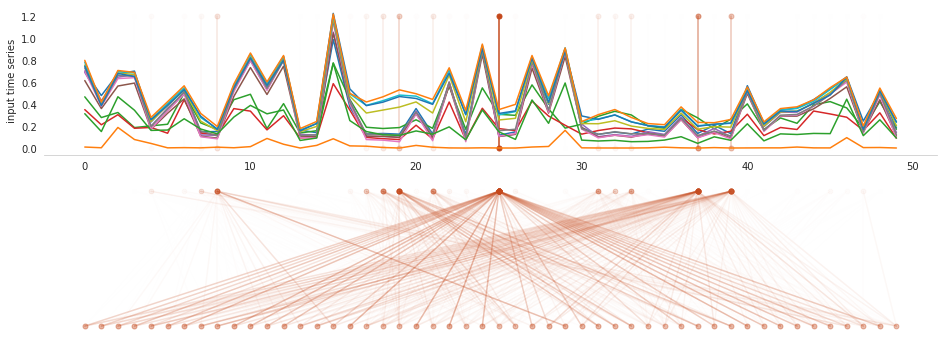
\includegraphics[width=\textwidth]{images/head0_conn_input}
		}
	\end{columns}
\end{frame}

\begin{frame}
	\frametitle{Choosing Observation Period}
	While we \textbf{learn} our \textbf{features} from \textbf{data}, we use \textbf{hand-chosen observation periods} to select the data.
%	\begin{itemize}
%		\item the observation period is usually chosen manually and conservatively (e.g. January to December)
%		\item some crop classes may be distinguishable earlier than others
%		\item with data every few days, earlier classifications may make classification results available months earlier
%	\end{itemize}
	\begin{tikzpicture}
		\node[inner sep=0](map){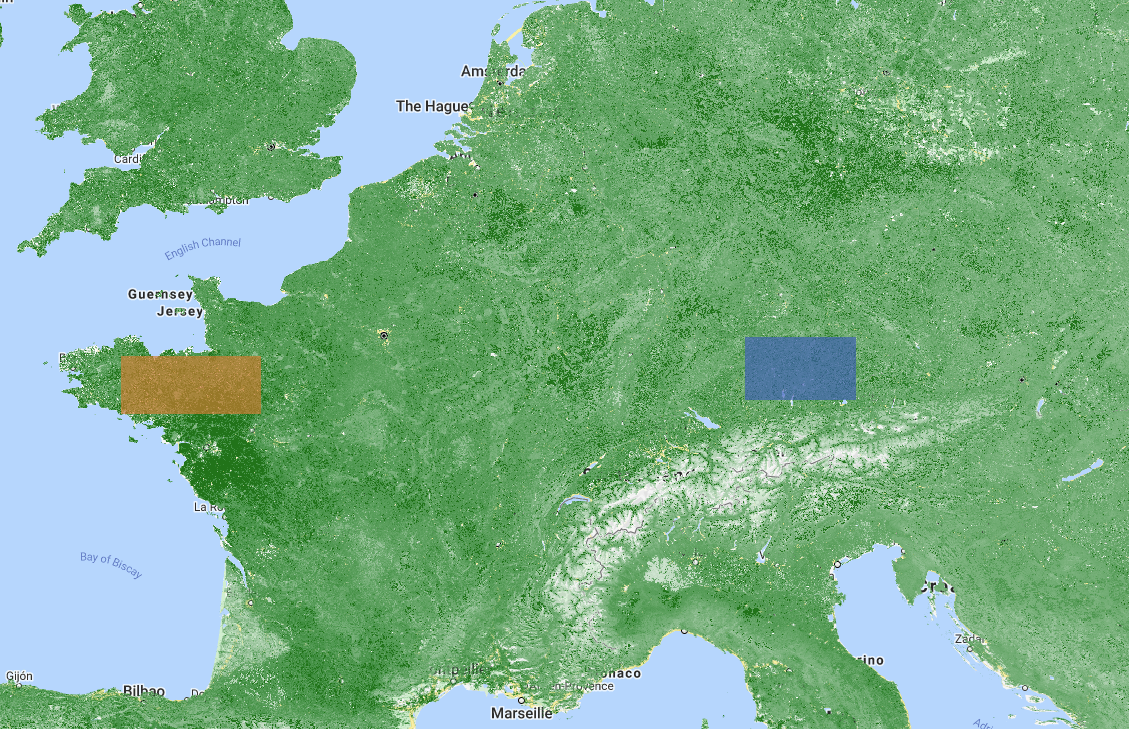
\includegraphics[width=9cm]{images/greenup/greenup_map}};
		\node[fill=white, opacity=0.9, text opacity=1] at (7,0){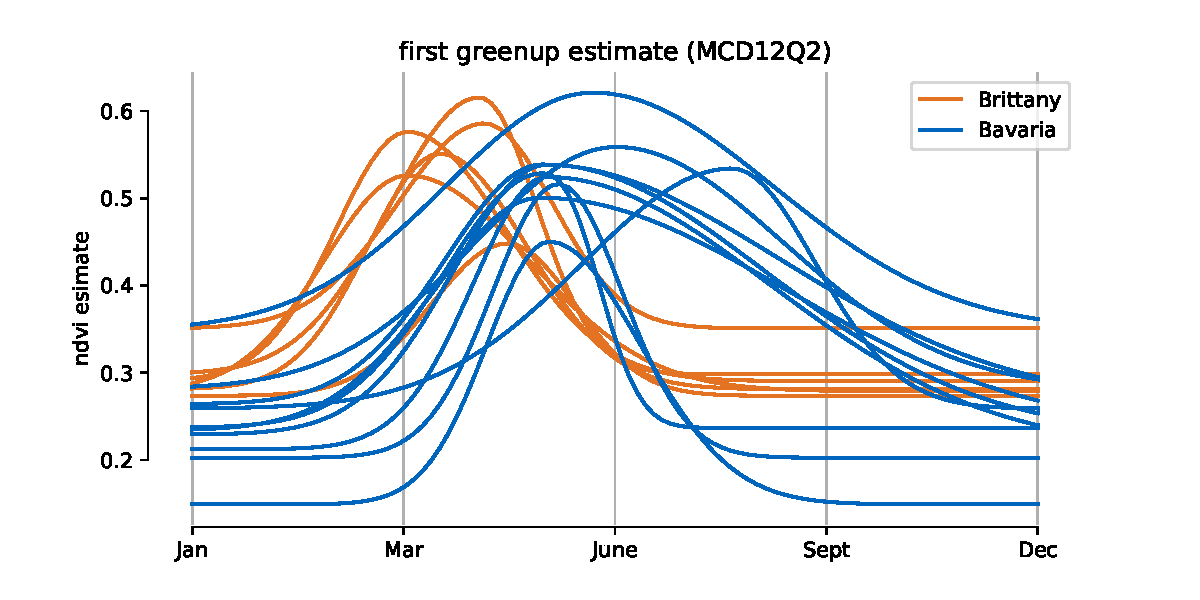
\includegraphics[width=8cm]{images/greenup/greenup_plots}};
		\node[anchor=north west, font=\scriptsize] at (map.south west){Day of first greenup (Modis product MCD12Q2)};
	\end{tikzpicture}
\end{frame}

%\begin{frame}
%	\frametitle{Related Work}
%	\begin{columns}
%		\column{.5\textwidth}
%		Remote Sensing
%		
%		large-scale datasets.
%		\column{.5\textwidth}
%		Time Series Community
%		
%		tested on small datasets from many applications.
%	\end{columns}
%\end{frame}


{\setbeamercolor{background canvas}{bg=tumbluedark}
	\begin{frame}[plain]
	
	\vfill
	\Huge\color{white}
	\begin{center}
		\begin{columns}
			\column{.5\textwidth}
			\vspace{7em}
			
			\hfill 
			Early Classification
			\column{.5\textwidth}
			
			%\includegraphics[width=7cm]{images/fdl}
		\end{columns}
	\end{center}
	
	\vfill
\end{frame}
}



\tikzstyle{rnn}=[draw,circle]
\tikzstyle{annot}=[rounded corners, fill=colorblue!20]
\colorlet{colortrain}{colorblue}
\colorlet{colorinfer}{colororange}
\tikzstyle{infer}=[-stealth, shorten >=.0em, shorten <=.0em, colorinfer]
\tikzstyle{loss}=[fill=colorblue!10, rounded corners, font=\small]
\tikzstyle{grad}=[colortrain]

\newcommand{\classimagepair}[1]{
\def\sample{#1}
\begin{tikzpicture}[node distance=.2em]
\node[label=above:{inputs $\V{x}_t$}](a){\includegraphics[width=.5\textwidth]{images/classification_without_earliness/TwoPatterns30EpochsNoEarliness/sample_\sample_x.png}};
\node[label=above:{softmaxed class scores $\yhat_t$}, right=of a](b){\includegraphics[width=.5\textwidth]{images/classification_without_earliness/TwoPatterns30EpochsNoEarliness/sample_\sample_p(y).png}};

\visible<2->{
%\draw (-2,-2) to[grid with coordinates] (8,4);
\node[annot, yshift=3em](wiggle1) at ($ (a)!0.3!(b) $) {event \#1};
\draw (wiggle1) -- (-1.5,0);
\draw (wiggle1) -- (5.5,-1);
}
\visible<3->{
\node[annot, yshift=-5em](wiggle2) at ($ (a)!0.3!(b) $) {event \#2};
\draw (wiggle2) -- (1,0);
\draw (wiggle2) -- (7.5,0);
}

\visible<4->{
\draw[very thick] (8.5,-2) -- (8.5,2); 
\node[annot, yshift=-5em, anchor=east](stop) at (10,-1) {...we could stop here};
%		\draw[shorten >=1em] (stop)++(2,0.5) -- (8,0);
}
\end{tikzpicture}
}

\begin{frame}<presentation:1-4>{Class Predictions}
\classimagepair{0}
\end{frame}


\begin{frame}
\frametitle{Early Classification on Remote Sensing Data}
\begin{tikzpicture}
	
	\tikzstyle{annot} = [font=\tiny\sffamily, text=tumblue]
	\tikzstyle{point} = [thin, tumbluelight, shorten >= .25em, shorten <= .25em]
	
	% from /home/marc/projects/EV2019/images/example/tstop.txt
	\def\tstopv{0.6285714285714286}
	\def\class{winter barley}
	
	\begin{groupplot}[
	group style={
		group name=my plots,
		group size=1 by 2,
		columns=1,
		xlabels at=edge bottom,
		xticklabels at=edge bottom,
		vertical sep=1em,
	},
	ylabel near ticks,
	ylabel style={font=\sffamily\small, rotate=-90},
	width=\textwidth,
	height=4cm,
	axis x line=bottom,
	axis y line=left,
	enlarge x limits=0.01,
	xtick={0,0.25,0.5,0.75,1},
	xticklabels={January,April,June,Sepember,December},
	ymajorgrids,
	ymin=0, ymax=1.4
	]
	
	\nextgroupplot[thin,
		no marks,  
		ylabel={$\V{x}$},
		draw opacity=.8,
		smooth,
		legend columns=4,
		legend style={at={(.5,1)},anchor=south, line width=1pt, fill=tumblue!10}
		]
		 
	\addplot[b1color] table [x=t, y=B1, col sep=comma, forget plot] {images/example/input.csv};
	\addplot[b9color] table [x=t, y=B9, col sep=comma, forget plot] {images/example/input.csv};
	\addplot[b10color] table [x=t, y=B10, col sep=comma] {images/example/input.csv};
	
	\addplot[b11color] table [x=t, y=B11, col sep=comma, forget plot] {images/example/input.csv};
	\addplot[b12color] table [x=t, y=B12, col sep=comma] {images/example/input.csv};
	
	\addplot[b5color] table [x=t, y=B5, col sep=comma, forget plot] {images/example/input.csv};
	\addplot[b6color] table [x=t, y=B6, col sep=comma, forget plot] {images/example/input.csv};
	\addplot[b7color] table [x=t, y=B7, col sep=comma, forget plot] {images/example/input.csv};
	\addplot[b8color] table [x=t, y=B8, col sep=comma, forget plot] {images/example/input.csv};
	\addplot[b8Acolor] table [x=t, y=B8A, col sep=comma] {images/example/input.csv};
		
	\addplot[b2color] table [x=t, y=B2, col sep=comma, forget plot] {images/example/input.csv};
	\addplot[b3color] table [x=t, y=B3, col sep=comma, forget plot] {images/example/input.csv};
	\addplot[b4color] table [x=t, y=B4, col sep=comma] {images/example/input.csv};
	
	
	\draw[fill=white, draw=none, opacity=.5] (axis cs:\tstopv,0) rectangle (axis cs:1,1.1);
	
	\node[annot](cllab) at (axis cs:.2,1.3) {clouds (noise)};
	\draw[point] (cllab) -- (axis cs:.13,.7);
	\draw[point] (cllab) -- (axis cs:.25,.7);
	\draw[point] (cllab) -- (axis cs:.53,1);
	\draw[point] (cllab) -- (axis cs:.45,.85);
	
	\node[annot](glab) at (axis cs:.8,1.3) {ground (signal)};
	\draw[point] (glab) -- (axis cs:.38,.3);
	\draw[point] (glab) -- (axis cs:.21,.3);
	\draw[point] (glab) -- (axis cs:.7,.3);
	
	\draw (axis cs:\tstopv,0) -- (axis cs:\tstopv,1) node[above]{$\tstop$};
	
	
	
	\legend{3 atmospheric, 2 short-wave infrared, 5 near infrared, 3 visible bands}
	
	\nextgroupplot[thin,
		smooth,
		no marks, 
		ylabel={$\yhat$},
		legend style={at={(.5,-.2)},anchor=north, line width=1pt, fill=tumblue!10},
		legend columns=6]	
	
	\addplot[meadowcolor] table [x=t, y=meadows, col sep=comma] {images/example/proba.csv};
	\addplot[wbarleycolor, thick] table [x=t, y=winter barley, col sep=comma] {images/example/proba.csv};
	\addplot[corncolor] table [x=t, y=corn, col sep=comma] {images/example/proba.csv};
	\addplot[wheatcolor,] table [x=t, y=winter wheat, col sep=comma] {images/example/proba.csv};
	\addplot[sbarleycolor] table [x=t, y=summer barley, col sep=comma] {images/example/proba.csv};
	\addplot[clovercolor] table [x=t, y=clover, col sep=comma] {images/example/proba.csv};
	\addplot[triticalecolor] table [x=t, y=winter triticale, col sep=comma] {images/example/proba.csv};
	
	\draw[fill=white, draw=none, opacity=.5] (axis cs:\tstopv,0) rectangle (axis cs:1,1);
	
	\draw (axis cs:\tstopv,0) -- (axis cs:\tstopv,2.2);
	
	\node[annot](rand) at (axis cs:.1,.8) {first hints};
	\draw[point] (rand) -- (axis cs:.2,.15);
	
	\node[annot](wrong) at (axis cs:.17,1.1) {initially wrong predictions};
	\draw[point] (wrong) -- (axis cs:.25,.7);
	\draw[point] (wrong) -- (axis cs:.4,1);
	
	\node[annot, align=center](corrwait) at (axis cs:.4,1.3) {waiting for more data};
	\draw[point] (corrwait) -- (axis cs:.5,.8);
	
	\node[annot](corr) at (axis cs:.8,1.3) {seen enough data};
	\draw[point] (corr) -- (axis cs:.63,1);
	
	\legend{meadows,\textbf{winter barley},corn,winter wheat,summer barley,clover,winter triticale}
	
	
%	\addplot[thick,colorclassone, name path=y1] table[x=t, y=y1]{\mydata};
%	\addplot[thick,colorclasstwo, name path=y2] table[x=t, y=y2]{\mydata};
%	\addplot[thick,colorclassthree, name path=y3] table[x=t, y=y3]{\mydata};
%	\addplot[thick,colorclassfour, name path=y4] table[x=t, y=y4]{\mydata};
	%\addplot[colorblue!20] fill between[of = y1 and axis];
	%\addplot[colorhgray!20] fill between[of = y2 and axis];
	%\addplot[colorgreen!20] fill between[of = y3 and axis];
	%\addplot[colororange!20] fill between[of = y4 and axis];
	
	
	\end{groupplot}
	
	\end{tikzpicture}

\url{https://arxiv.org/abs/1901.10681}

\end{frame}

%\begin{frame}
%	\frametitle{Autoregressive Classification Model}
%	
%	\input{images/classmodel.tikz}
%	
%\end{frame}


{\setbeamercolor{background canvas}{bg=tumbluedark}
	\begin{frame}[plain]
	
	\vfill
	\Huge\color{white}
	\begin{center}
		\begin{columns}
			\column{.5\textwidth}
			\vspace{7em}
			
			\hfill 
			Method
			\column{.5\textwidth}
			
			%\includegraphics[width=7cm]{images/fdl}
		\end{columns}
	\end{center}
	
	\vfill
\end{frame}
}

\begin{frame}<presentation:-4>
\frametitle{Augmenting Classification Models}

\begin{columns}
	
	\column{.5\textwidth}
	\begin{center}
		
		\begin{tikzpicture}[node distance=1em and 1.5em]
\node[](x0){$x_t$};
\node[rnn, below=of x0](h0){\small$f\left(\xuptot\right)$};
\node[below right= 2em and .0em of h0](y0){$\yhat_t$};
\node[rnn, left=2em of h0,draw=lightgray](hprev){};
\node[rnn, right=2em of h0,draw=lightgray](hnext){};

\draw[infer] (x0) -- (h0);
\draw[infer,draw=lightgray] (hprev) -- (h0);
\draw[infer,draw=lightgray] (h0) -- (hnext);
\draw[infer] (h0) -- (y0) node[midway,right, text=black](wc){$\theta_{cl}$};

\visible<2->{
\node[below left= 2em and .0em of h0](d0){$\delta_t$};
\draw[infer] (h0) -- (d0) node[midway,left, text=black](wd){$\theta_{\delta}$};
}

\visible<3->{
	\node[loss, below=of y0](L0){$\mathcal{L}_{cl}(\yhat,\V{y})$};
	%\node[right=of L0](t0){$\V{y}_t$};
	\draw[-stealth, grad] (y0) -- (L0);
	%\draw[-stealth, grad] (t0) -- (L0);
	%\draw[-stealth, grad] (L0) to [in=-25, out=25, looseness=2] node[midway, right, text=colortrain]{$\frac{\partial\mathcal{L}_{cl}}{\partial\theta_\text{rnn}}$}
	%(h0);
	
	\draw[-stealth, grad] (L0) to [bend right=30] node[near end, right, text=colortrain]{$\frac{\partial\mathcal{L}_{cl}}{\partial\theta_\text{cl}}$}
	(wc);
}

\only<4>{
\node[below=7em of h0, loss](L){$\mathcal{L}(\V{y_t},\yhat_t)$};
\draw[infer] (L0) -- (L);
\draw[infer] (d0) -- (L);

\draw[-stealth, grad] (L) to [bend right=30] node[midway, right, text=colortrain]{$\frac{\partial\mathcal{L}}{\partial\mathcal{L}_{cl}}$}
(L0);

\draw[-stealth, grad] (L) to [bend left=30] node[midway, left, text=colortrain]{$\frac{\partial\mathcal{L}}{\partial\theta_\delta}$}
(wd);

}

\only<5->{

\node[below=of d0](pt){$P(t)$};
\node[below=8em of h0, loss](L){$\mathcal{L}(\V{y_t},\yhat_t) = P(t)\mathcal{L}_{cl}(\V{y_t},\yhat_t)$};


\draw[infer] (L0) -- (L);
\draw[infer] (d0) -- (pt);
\draw[infer] (pt) -- (L);

%}
%
\only<5->{
\node[left=.5em of pt](budget){\small $\prod_{t'<t}(1-\delta_{t'})$};
\draw[infer] (budget) -- (pt);}

%\only<7->{
%	\node[left=.5em of pt](budget){$\mathcal{B}_{t-1}$};
%	
%}

\draw[-stealth, grad] (L) to [bend right=30] node[midway, right, text=colortrain]{$\frac{\partial\mathcal{L}}{\partial\mathcal{L}_{cl}}$}
(L0);

\draw[-stealth, grad] (L) to [bend left=30] node[midway, left, text=colortrain]{$\frac{\partial\mathcal{L}}{\partial P(t)}$}
(pt);

\draw[-stealth, grad] (pt) to [bend left=30] node[midway, left, text=colortrain]{$\frac{\partial P(t)}{\partial \theta_{\delta}}$}
(wd);

}

\end{tikzpicture}

	\end{center}
	\column{.5\textwidth}
	\begin{tikzpicture}

\pgfplotstableread[col sep = comma]{images/qualitative_example/early_rnn_run-sample0.csv}\mydata

\begin{groupplot}[
	group style={
		group name=my plots,
		group size=1 by 5,
		columns=1,
		xlabels at=edge bottom,
		xticklabels at=edge bottom,
		vertical sep=5pt,
	},
	ylabel near ticks,
	ylabel style={rotate=-90},
	width=\textwidth,
	height=3cm,
	axis x line=bottom,
	axis y line=left,
	enlarge x limits=0.01,
	ymajorgrids,
]

\nextgroupplot[no marks, enlarge y limits=0.05, hide x axis, ylabel={$x$}]
\addplot[thick, tumblue] table[x=t, y=x]{\mydata};

\nextgroupplot[no marks, ylabel={$\yhat_t$}, enlarge y limits=0.05, hide x axis]	
\addplot[thick,colorclassone, name path=y1] table[x=t, y=y1]{\mydata};
\addplot[thick,colorclasstwo, name path=y2] table[x=t, y=y2]{\mydata};
\addplot[thick,colorclassthree, name path=y3] table[x=t, y=y3]{\mydata};
\addplot[thick,colorclassfour, name path=y4] table[x=t, y=y4]{\mydata};

%\addplot[colorblue!20] fill between[of = y1 and axis];
%\addplot[colorhgray!20] fill between[of = y2 and axis];
%\addplot[colorgreen!20] fill between[of = y3 and axis];
%\addplot[colororange!20] fill between[of = y4 and axis];
\only<2->{
\nextgroupplot[ybar, bar width=1pt, ylabel={$\delta_t$}]
\addplot[draw=none, fill=tumblue] table[x=t, y=dt]{\mydata};
}

\only<5->{
\nextgroupplot[ybar, bar width=1pt, hide x axis, ylabel={$P(t)$}]
\addplot[draw=none, fill=tumblue] table[x=t, y=pts]{\mydata};

%\nextgroupplot[ybar, bar width=1pt, hide x axis, ylabel={$\prod_{t'<t}(1-\delta_{t'})$}]
%\addplot[draw=none, fill=tumblue, xlabel={time $t$}] table[x=t, y=Bt]{\mydata};
}

\end{groupplot}

\end{tikzpicture}

	
	
\end{columns}

\end{frame}
%
%\begin{frame}
%\frametitle{Impact of Early Classification on Vegetation Data}
%
%\Large
%
%\begin{itemize}[itemsep=1em]
%\item<1-> \textbf{supervised end-to-end} learning scenario
%\item<2-> we get a stopping time \textbf{for free} solely from classifying labels
%\item<3-> relate to \textbf{characteristic features}, i.e., \textbf{crop phenology}
%\item<4-> next: assess seasonal shifts in \textbf{vegetation phenology} due to \textbf{environmental conditions}
%\end{itemize}
%
%\end{frame}

\begin{frame}
	\frametitle{Loss functions}
	
	{
	\Large
	
	\begin{equation*}
		\mathcal{L}(\M{X}, \V{y}) = \sum_{t=1}^{T} P(t) \left( \mathcal{L}_c (\xuptot, \V{y}) - \mathcal{R}_e(t, \ycorrect_t) \right)
	\end{equation*} 
	
	earlyness reward: $ \mathcal{R}_e(t, \ycorrect_t) = \ycorrect_t \left(1 - \frac{t}{T}\right) $	
	classificaiton loss: $-\log(\ycorrect_t)$ (aka. cross entropy)
	
	}

	\vspace{1em}

	\Large
	\begin{itemize}
		\item $\M{X}=(\V{x}_1,\V{x}_2,\dots,\V{x}_T)$: entire time series of observations $\V{x}$
		\item $\xuptot=(\V{x}_1,\V{x}_2,\dots,\V{x}_t)$: time series until time $t$
		\item $\V{y} \in \{0,1\}^C$: one-hot vector of the classes
		\item $\ycorrect \in [0,1]$: prediction score of the correct class
	\end{itemize}
	
	
\end{frame}

{\setbeamercolor{background canvas}{bg=tumbluedark}
	\begin{frame}[plain]
	
	\vfill
	\Huge\color{white}
	\begin{center}
		\begin{columns}
			\column{.5\textwidth}
			\vspace{7em}
			
			\hfill 
			Results
			\column{.5\textwidth}
			
			%\includegraphics[width=7cm]{images/fdl}
		\end{columns}
	\end{center}
	
	\vfill
\end{frame}
}

%\begin{frame}
%
%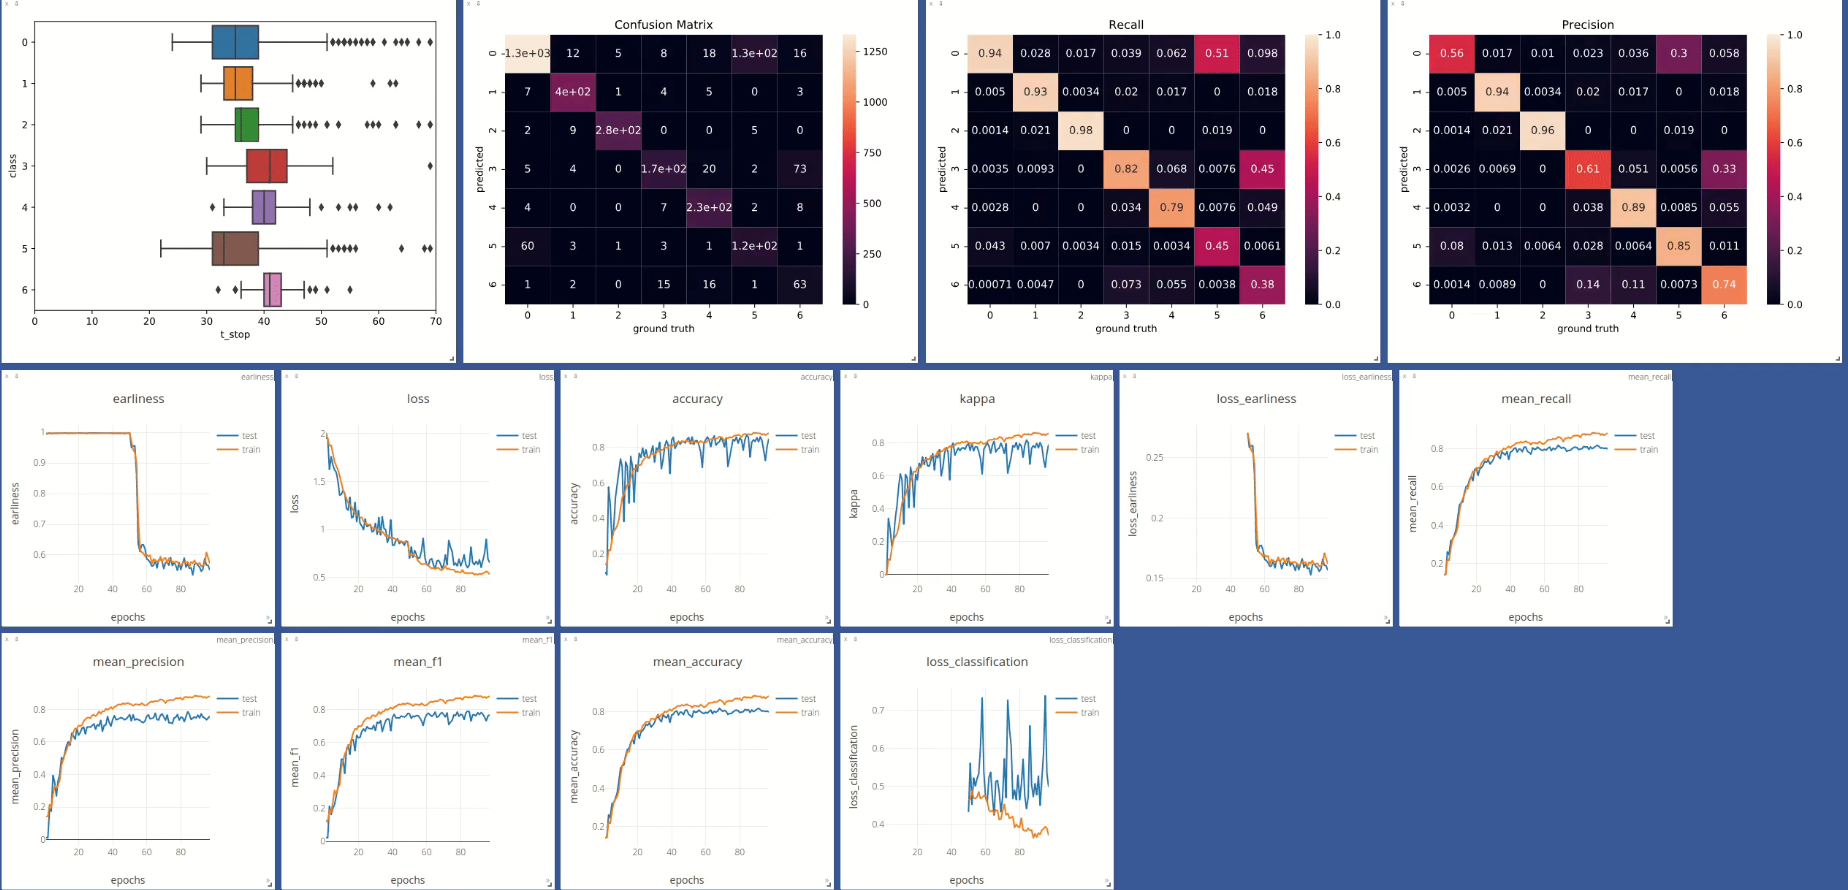
\includegraphics[width=\textwidth]{mp4/run_twophase_fast.png}
%\end{frame}

\begin{frame}
	
%	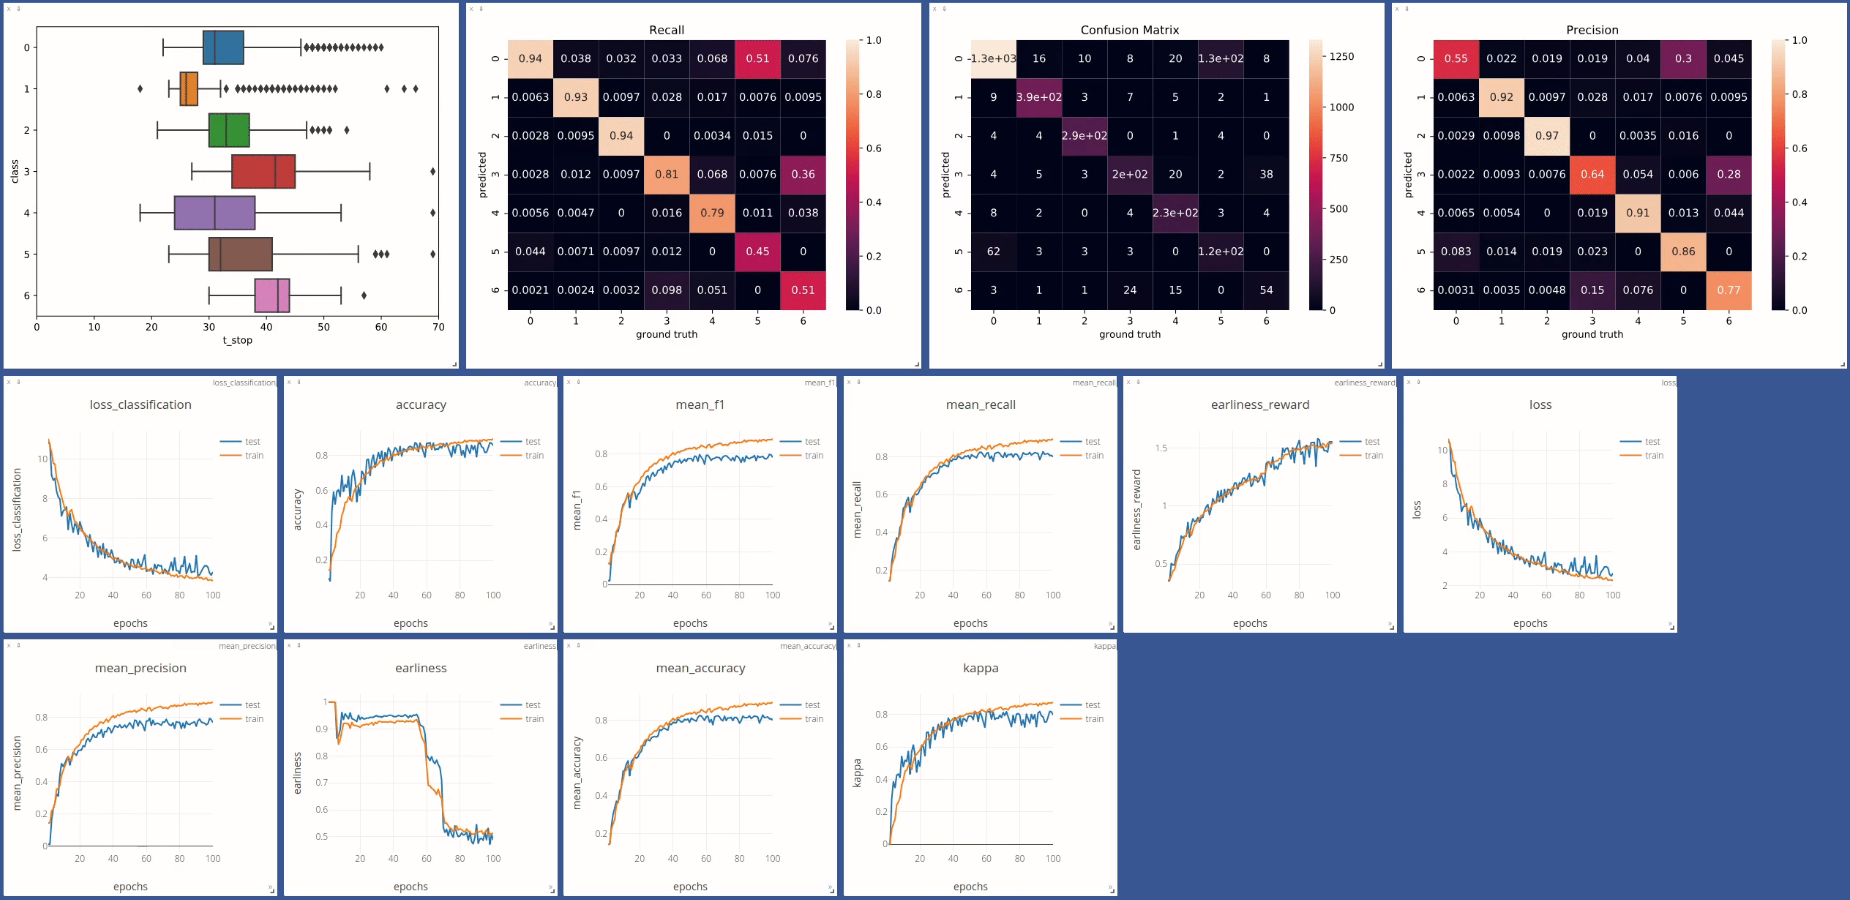
\includegraphics[width=\textwidth]{mp4/run_earyreward_fast.png}
	
	\includemedia[
	width=\textwidth,
	activate=pageopen,
	addresource=mp4/run_earyreward_fast.mp4,
	flashvars={source=mp4/run_earyreward_fast.mp4&loop=true&
		autoPlay=true}
	]{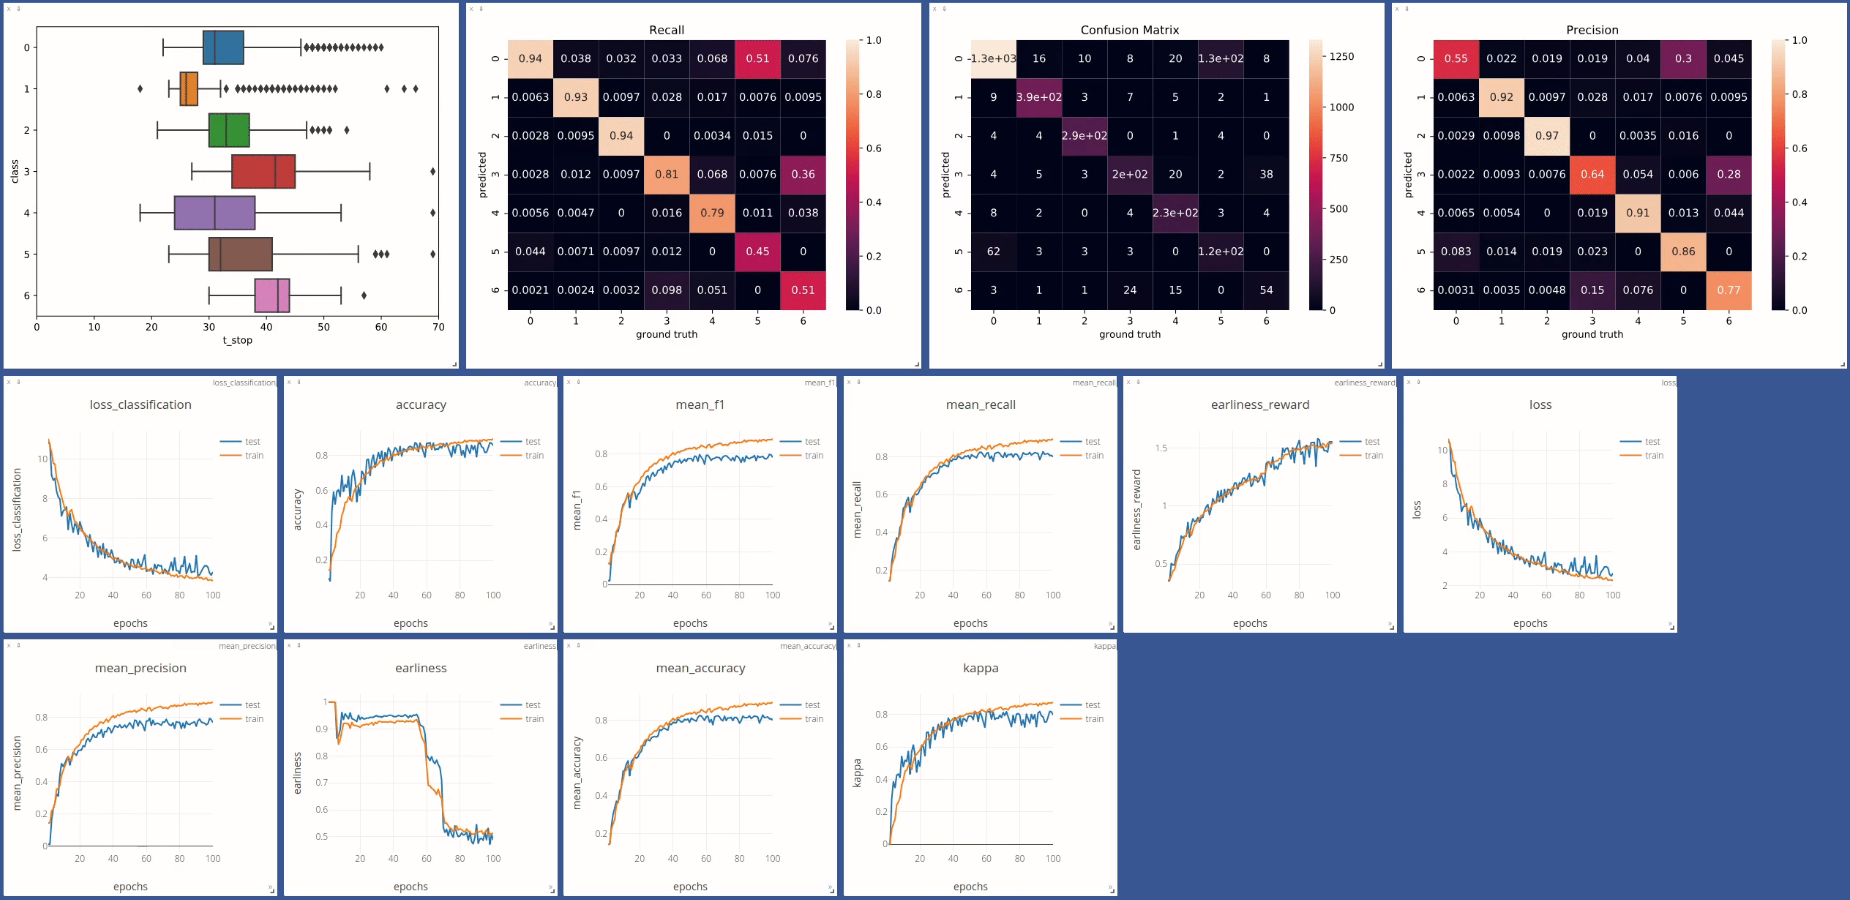
\includegraphics[width=\textwidth]{mp4/run_earyreward_fast.png}}{mp4/run_earyreward_fast.mp4}
	
	
\end{frame}


%
%\begin{frame}
%	
%	
%	\newcommand{\figearlyreward}{
\def\datapath{images/logs/data/early_reward_p2/classes}
\tikzsetnextfilename{loss-accuracyplots}
\begin{tikzpicture}
	\begin{groupplot}[
	group style = {
		group size = 1 by 2,
		x descriptions at=edge bottom,
		vertical sep=1em},
	no markers,
	height=4cm,
%	legend style={at={(0.03,0.5)},anchor=west},
	width=\linewidth,
	xlabel=epochs
 	]
	\nextgroupplot[legend columns=3, ylabel=loss]

	\addplot[test, tumblack] table [x=epoch, y=loss, col sep=comma] {\datapath/log_earliness_test.csv};
	
	\addplot[test, accuracycolor] table [x=epoch, y=loss_classification, col sep=comma] {\datapath/log_earliness_test.csv};
	
	\addplot[test, earlinesscolor] table [x=epoch, y=earliness_reward, col sep=comma] {\datapath/log_earliness_test.csv};
	
%	\legend{total loss (eval), classification loss (eval), earliness reward (eval)}
%	
	\legend{$(\mathcal{L}_\text{c} - \mathcal{R}_\text{e})$, $\mathcal{L}_\text{c}$, $\mathcal{R}_\text{e}$}
	
	
	
	\nextgroupplot[
		legend columns=2, 
		legend pos=south east,
		ytick={0,0.5,1},
		yticklabels={
			0 ({\color{earlinesscolor} jan}),
			0.5 ({\color{earlinesscolor} jun}),
			1 ({\color{earlinesscolor} dec})},
		ylabel=accuracy/$\meantstop$]
	\addplot[test, accuracycolor] table [x=epoch, y=accuracy, col sep=comma] {\datapath/log_earliness_test.csv};
	\addplot[test, earlinesscolor] table [x=epoch, y=earliness, col sep=comma] {\datapath/log_earliness_test.csv};

	\legend{accuracy,$\meantstop$}
	
	\end{groupplot}
\end{tikzpicture}

}

\newcommand{\figtwophasecrossentropy}{
\begin{tikzpicture}
\begin{groupplot}[
group style = {
	group size = 1 by 2,
	x descriptions at=edge bottom,
	vertical sep=1em},
no markers,
height=2.8cm,
%	legend style={at={(0.03,0.5)},anchor=west},
width=\linewidth,
ymin=0,ymax=2.5,
xlabel=epochs
]
\nextgroupplot[legend columns=3, ylabel=loss,
legend style={at={(1,.85)}, anchor=north east}]

\addplot[test, tumblack] table [x=epoch, y=loss, col sep=comma] {images/logs/data/twophasecrossentropy/log_earliness_test.csv};

\addplot[test, accuracycolor] table [x=epoch, y=loss_classification, col sep=comma] {images/logs/data/twophasecrossentropy/log_earliness_test.csv};

\addplot[test, earlinesscolor] table [x=epoch, y=loss_earliness, col sep=comma] {images/logs/data/twophasecrossentropy/log_earliness_test.csv};

\draw[draw, thick] (axis cs:50,0) -- (axis cs:50,2) node[above, font=\sffamily\scriptsize](s){switch epoch};
\node[left=1em of s, font=\sffamily\scriptsize]{accuracy only};
\node[right=1em of s, font=\sffamily\scriptsize]{accuracy+earliness};

\legend{$(\mathcal{L}_\text{c} + \mathcal{L}_\text{e})$, $\mathcal{L}_\text{c}$, $\mathcal{L}_\text{e}$}

\nextgroupplot[
legend columns=2, 
ytick={0,0.5,1},
ymin=0,ymax=1,
legend style={at={(1,0)}, anchor=south east},
yticklabels={
	0 ({\color{earlinesscolor} jan}),
	0.5 ({\color{earlinesscolor} jun}),
	1 ({\color{earlinesscolor} dec})},
ylabel=accuracy/$\meantstop$]
\addplot[test, accuracycolor] table [x=epoch, y=accuracy, col sep=comma] {images/logs/data/twophasecrossentropy/log_earliness_test.csv};
\addplot[test, earlinesscolor] table [x=epoch, y=earliness, col sep=comma] {images/logs/data/twophasecrossentropy/log_earliness_test.csv};

\legend{accuracy,$\meantstop$}

\draw[draw, thick] (axis cs:50,0) -- (axis cs:50,1.1);

\end{groupplot}
\end{tikzpicture}

}
%
%
%	\begin{columns}
%%	\column{.5\textwidth}
%%\figtwophasecrossentropy
%%{two-phase training first optimizing for accuracy-only and then for early classifications as well using \emph{lateness penalty} loss.}
%
%	\column{\textwidth}
%\figearlyreward
%{one training phase using the \emph{earliness reward} formulation.}
%\end{columns}
%	
%\end{frame}
%
%\begin{frame}
%	
%	
%		\def\datapath{images/logs/data/early_reward_p2/classes}

\tikzsetnextfilename{trainingstoppingclasses}
\begin{tikzpicture}
	\begin{groupplot}[
	group style = {
		group size = 1 by 7,
		x descriptions at=edge bottom,
		vertical sep=.75em},
	title style={
		font=\sffamily\scriptsize,
		at={(0,1)},
		anchor=north west
	},
	ymajorgrids,
	no markers,
	height=2.7cm,
	legend style={at={(0.5,1)},anchor=south},
	width=\linewidth,
	xlabel=epochs,
	ymax=1.1,
	ymin=0.3,
	ylabel=$\tstop$,
	ytick={0,0.25,0.5,0.75,1},
	yticklabels={Jan,Apr,Jun,Sep,Dec}
	]
	\nextgroupplot[title=meadows, legend columns=3]
	\addplot[meancolor] table [x=epoch, y=meadows, col sep=comma] {\datapath/mean.csv};
	\addplot[mediancolor] table [x=epoch, y=meadows, col sep=comma] {\datapath/median.csv};
	\addplot+[name path=upper, draw=none,forget plot] table [x=epoch, y=meadows, col sep=comma] {\datapath/mean+std.csv};
	\addplot+[name path=lower, draw=none,forget plot] table [x=epoch, y=meadows, col sep=comma] {\datapath/mean-std.csv};
	\addplot[stdcolor] fill between[of=lower and upper];
	
	\legend{mean, median, mean $\mp$ std}
	
	\nextgroupplot[title=winter barley]
	\addplot[meancolor] table [x=epoch, y=winter barley, col sep=comma] {\datapath/mean.csv};
	\addplot[mediancolor] table [x=epoch, y=winter barley, col sep=comma] {\datapath/median.csv};
	\addplot+[name path=upper, draw=none] table [x=epoch, y=winter barley, col sep=comma] {\datapath/mean+std.csv};
	\addplot+[name path=lower, draw=none] table [x=epoch, y=winter barley, col sep=comma] {\datapath/mean-std.csv};
	\addplot[stdcolor] fill between[of=lower and upper];
	\nextgroupplot[title=corn]
%	\addplot table [x=epoch, y=corn, col sep=comma] {images/logs/data/early_reward/classes/mean.csv};
	
	\addplot[meancolor] table [x=epoch, y=corn, col sep=comma] {\datapath/mean.csv};
	\addplot[mediancolor] table [x=epoch, y=corn, col sep=comma] {\datapath/median.csv};
	\addplot+[name path=upper, draw=none] table [x=epoch, y=corn, col sep=comma] {\datapath/mean+std.csv};
	\addplot+[name path=lower, draw=none] table [x=epoch, y=corn, col sep=comma] {\datapath/mean-std.csv};
	\addplot[stdcolor] fill between[of=lower and upper];
	
	\nextgroupplot[title=winter wheat]
%	\addplot table [x=epoch, y=winter wheat, col sep=comma] {images/logs/data/early_reward/classes/mean.csv};
%	
	\addplot[meancolor] table [x=epoch, y=winter wheat, col sep=comma] {\datapath/mean.csv};
	\addplot[mediancolor] table [x=epoch, y=winter wheat, col sep=comma] {\datapath/median.csv};
	\addplot+[name path=upper, draw=none] table [x=epoch, y=winter wheat, col sep=comma] {\datapath/mean+std.csv};
	\addplot+[name path=lower, draw=none] table [x=epoch, y=winter wheat, col sep=comma] {\datapath/mean-std.csv};
	\addplot[stdcolor] fill between[of=lower and upper];
	
	\nextgroupplot[title=summer barley]
%	\addplot table [x=epoch, y=winter barley, col sep=comma] {images/logs/data/early_reward/classes/mean.csv};
	
	\addplot[meancolor] table [x=epoch, y=summer barley, col sep=comma] {\datapath/mean.csv};
	\addplot[mediancolor] table [x=epoch, y=summer barley, col sep=comma] {\datapath/median.csv};
	\addplot+[name path=upper, draw=none] table [x=epoch, y=summer barley, col sep=comma] {\datapath/mean+std.csv};
	\addplot+[name path=lower, draw=none] table [x=epoch, y=summer barley, col sep=comma] {\datapath/mean-std.csv};
	\addplot[stdcolor] fill between[of=lower and upper];
	
	\nextgroupplot[title=clover]
%	\addplot table [x=epoch, y=clover, col sep=comma] {images/logs/data/early_reward/classes/mean.csv};
	
	\addplot[meancolor] table [x=epoch, y=clover, col sep=comma] {\datapath/mean.csv};
	\addplot[mediancolor] table [x=epoch, y=clover, col sep=comma] {\datapath/median.csv};
	\addplot+[name path=upper, draw=none] table [x=epoch, y=clover, col sep=comma] {\datapath/mean+std.csv};
	\addplot+[name path=lower, draw=none] table [x=epoch, y=clover, col sep=comma] {\datapath/mean-std.csv};
	\addplot[stdcolor] fill between[of=lower and upper];
	
	\nextgroupplot[title=winter triticale]
%	\addplot table [x=epoch, y=winter triticale, col sep=comma] {images/logs/data/early_reward/classes/mean.csv};

	\addplot[meancolor] table [x=epoch, y=winter triticale, col sep=comma] {\datapath/mean.csv};
	\addplot[mediancolor] table [x=epoch, y=winter triticale, col sep=comma] {\datapath/median.csv};
	\addplot+[name path=upper, draw=none,forget plot] table [x=epoch, y=winter triticale, col sep=comma] {\datapath/mean+std.csv};
	\addplot+[name path=lower, draw=none,forget plot] table [x=epoch, y=winter triticale, col sep=comma] {\datapath/mean-std.csv};
	\addplot[stdcolor] fill between[of=lower and upper];

	
	\end{groupplot}
	\end{tikzpicture}
%		{Class-wise analysis of the estimated stopping time during training in the evaluation set.}
%	
%\end{frame}

\begin{frame}
\frametitle{Stopping times per crop Class}

%\tikzsetnextfilename{classboxplots}

\tikzstyle{druschdatum} = [thin, star,star points=3, star point ratio=0.5, inner sep=.15em, draw=tumwhite, fill=tumblue]

\newcommand{\druschdatum}{
	\begin{tikzpicture}[scale=2, baseline=-.25em, inner sep=0]
	\node[druschdatum, inner sep=.25em]{};
	\end{tikzpicture}
}


\begin{tikzpicture}

\tikzstyle{boxstyle}=[
	mark options={
	draw=tumblue,
	scale=0.5},
	mark=*,
	solid,
	draw=black]

\begin{axis}[
ytick={1,2,3,4,5,6,7},
yticklabels={
	meadows,
	winter barley,
	corn,
	winter wheat,
	summer barley,
	clover,
	winter triticale},
xmajorgrids,
height=6cm,
xmin = 0,
xmax = 1,
ymin = 1,
ymax = 8,
width=\linewidth,
y axis line style={draw=none},
xtick={0,0.1666666667,0.4166666667,0.6666666667,0.9166666667},
xticklabels={January,March,June,September,December},
xlabel={stopping date $\tstop$}
]


%% august <- recommended end of period
% 0.6666666667
\draw [fill=tumbluelight, opacity=.4, draw=none] (axis cs:0.1666666667,0) rectangle (axis cs:0.5833333333,8);
\draw[draw=tumgraydark] (axis cs:0.5833333333,0) -- (axis cs:0.5833333333,8);

\node[font=\tiny\sffamily] at (axis cs:0.37,8.2){vegetative season};

%\node[font=\tiny\sffamily] at (axis cs:0.8,8.2){b};


\addplot+[boxplot, fill=meadowcolor, boxstyle] table[x = meadows, col sep=comma]{images/logs/data/early_reward_p2/classes/meadows.csv};
%
%\addplot+[fill=meadowcolor, draw=black,
%boxplot prepared={
%median=0.4857142857142857,
%upper quartile=0.4,
%lower quartile=0.5857142857142857,
%upper whisker=0.8642857142857143,
%lower whisker=0.12142857142857144,
%} ] coordinates {};

\addplot+[boxplot, fill=wbarleycolor, boxstyle] table[x=winter barley, col sep=comma]{images/logs/data/early_reward_p2/classes/winter_barley.csv};


%
%\addplot+[fill=wbarleycolor, draw=black,
%boxplot prepared={
%median=0.42857142857142855,
%upper quartile=0.37142857142857144,
%lower quartile=0.5857142857142857,
%upper whisker=0.9071428571428573,
%lower whisker=0.04999999999999999,
%} ] coordinates {};


\addplot+[boxplot, fill=corncolor, boxstyle] table[x =corn, col sep=comma]{images/logs/data/early_reward_p2/classes/corn.csv};
%
%\addplot+[fill=corncolor, draw=black,
%boxplot prepared={
%median=0.45714285714285713,
%upper quartile=0.42857142857142855,
%lower quartile=0.5142857142857142,
%upper whisker=0.6428571428571428,
%lower whisker=0.30000000000000004,
%} ] coordinates {};

\addplot+[boxplot, fill=wheatcolor, boxstyle] table[x =winter wheat, col sep=comma]{images/logs/data/early_reward_p2/classes/winter_wheat.csv};


%
%\addplot+[fill=wheatcolor, draw=black,
%boxplot prepared={
%median=0.5285714285714286,
%upper quartile=0.45714285714285713,
%lower quartile=0.5857142857142857,
%upper whisker=0.7785714285714287,
%lower whisker=0.26428571428571423,
%} ] coordinates {};

\addplot+[boxplot, fill=sbarleycolor, boxstyle] table[x =summer barley, col sep=comma]{images/logs/data/early_reward_p2/classes/summer_barley.csv};

%\addplot+[fill=sbarleycolor, draw=black,
%boxplot prepared={
%median=0.37142857142857144,
%upper quartile=0.2857142857142857,
%lower quartile=0.5428571428571428,
%upper whisker=0.9285714285714285,
%lower whisker=-0.09999999999999998,
%} ] coordinates {};

\addplot+[boxplot, fill=clovercolor, boxstyle] table[x=clover, col sep=comma]{images/logs/data/early_reward_p2/classes/clover.csv};

%\addplot+[fill=clovercolor, draw=black,solid,
%boxplot prepared={
%median=0.5,
%upper quartile=0.42857142857142855,
%lower quartile=0.6142857142857143,
%upper whisker=0.892857142857143,
%lower whisker=0.14999999999999986,
%} ] coordinates {};

\addplot+[boxplot, fill=triticalecolor, boxstyle] table[x=winter triticale, col sep=comma]{images/logs/data/early_reward_p2/classes/winter_triticale.csv};

\def\triticale{0.5722222222}
\def\sbarley{0.5833333333}
\def\wbarley{0.5388888889}
\def\wheat{0.5694444444}


% triticale drusch datum 26.07.
%\draw (axis cs:0.524537037,6.5) -- (axis cs:0.524537037,7.5);
\node[druschdatum] at (axis cs:\triticale,7){};

%  summer barley drusch datum 1.8.
%\draw (axis cs:\sbarley,4.5) -- (axis cs:\sbarley,5.5);
\node[druschdatum] at (axis cs:\sbarley,5){};


% winter wheat drusch datum 26.07.
%\draw (axis cs:\wheat,3.5) -- (axis cs:\wheat,4.5);
\node[druschdatum] at (axis cs:\wheat,4){};


% winter barley datum 15.07.
%\draw (axis cs:\wbarley,1.5) -- (axis cs:\wbarley,2.5);
\node[druschdatum] at (axis cs:\wbarley,2){};


%\addplot+[fill=triticalecolor, draw=black,solid,
%boxplot prepared={
%median=0.5571428571428572,
%upper quartile=0.5142857142857142,
%lower quartile=0.6142857142857143,
%upper whisker=0.7642857142857145,
%lower whisker=0.3642857142857141,
%} ] coordinates {};

\end{axis}
\end{tikzpicture} 

\end{frame}


%\begin{frame}
%	\frametitle{ICML AI for Social Good Workshop}
%	\begin{columns}
%	\column{.5\textwidth}
%	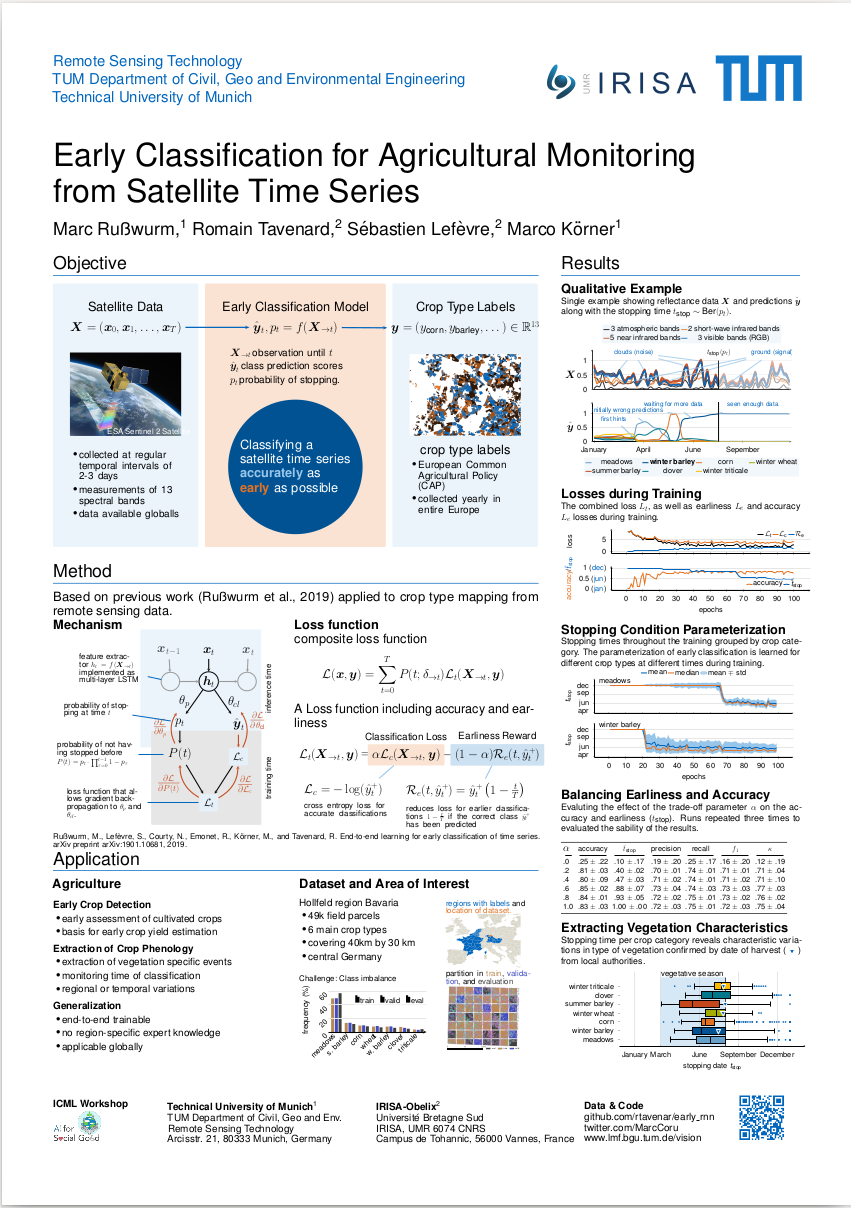
\includegraphics[width=.6\textwidth]{images/AI4SG_Poster}
%	
%	\column{.5\textwidth}
%	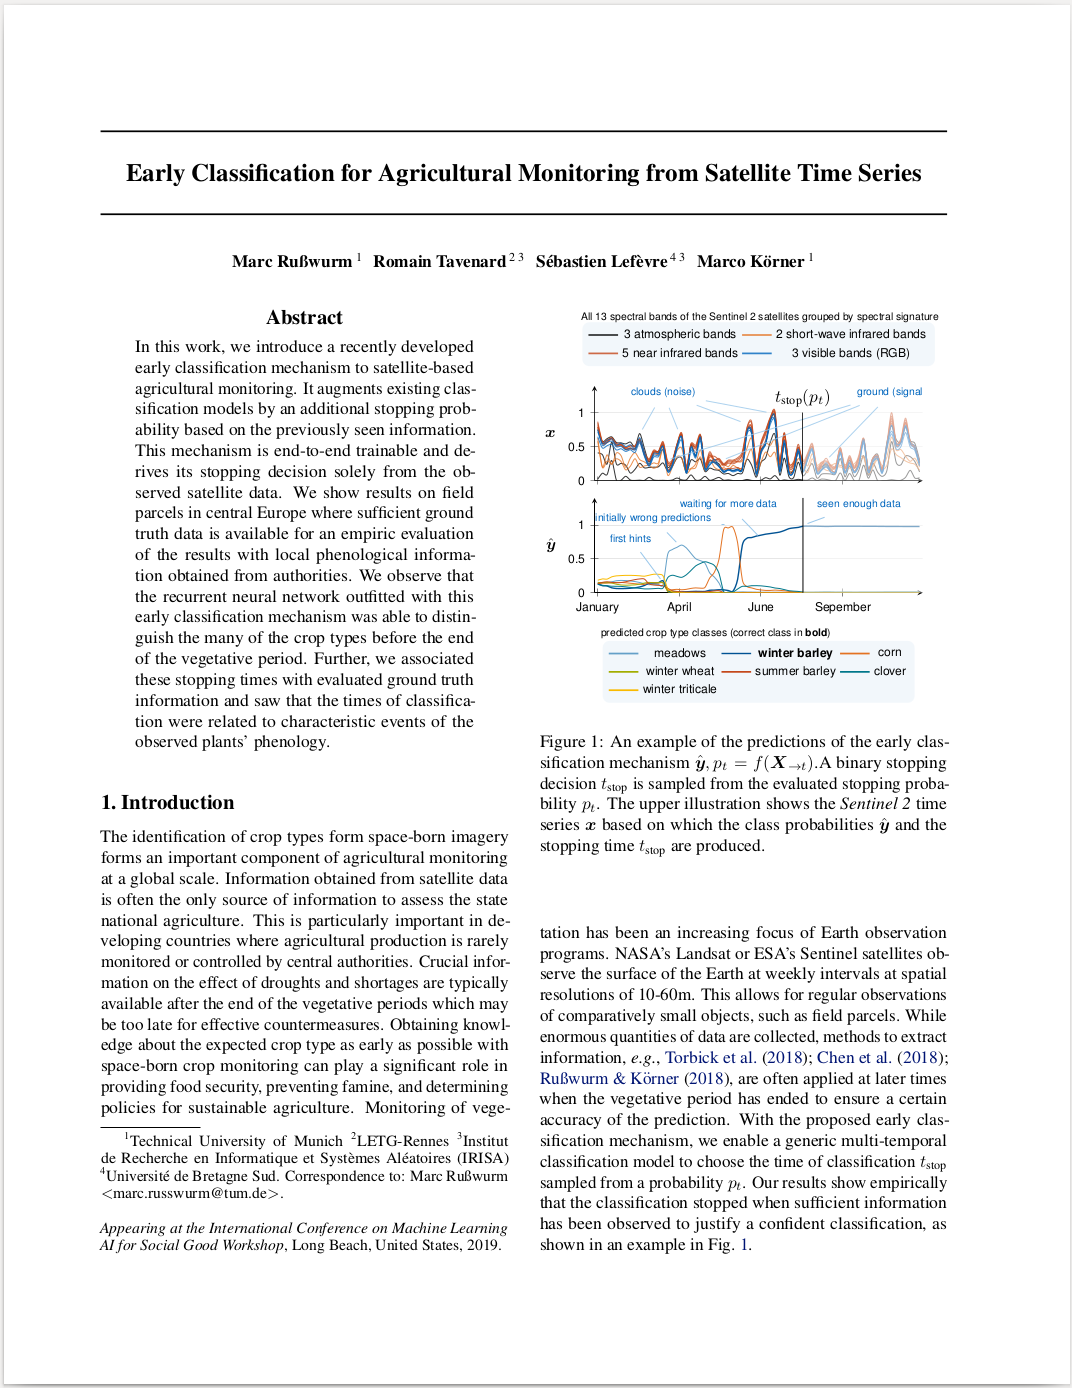
\includegraphics[width=.6\textwidth]{images/AI4SG_Paper}
%	
%%	\end{columns}
%\end{frame}

\begin{frame}
	\frametitle{Comparison of ELECTS (ours) to SR2-CF2 (Mori et al.)}
	\begin{tikzpicture}
%\pgfplotstableread[col sep = comma]{images/satellite_comparison/ELECTS_uniform.csv}\elects
%\pgfplotstableread[col sep = comma]{images/satellite_comparison/SR2CF2_uniform.csv}\mori

\begin{groupplot}[
group style={
	group size=3 by 1,
},
ymajorgrids,
legend columns=2,
width=.36\textwidth,
height=4cm,
ylabel style={yshift=-1.2em},
]

\nextgroupplot[
ylabel={accuracy},
xlabel={dataset size},
legend pos=south east]

\addplot[tumblue,mark=*] table[col sep = comma, x=nsamples, y=accuracy]{images/satellite_comparison/ELECTS_uniform.csv};
\addplot[tumorange,mark=*] table[col sep = comma, x=nsamples, y=accuracy]{images/satellite_comparison/SR2CF2_uniform.csv};

\legend{ELECTS,SR2-CF2}

\nextgroupplot[
ylabel={earliness},
xlabel={dataset size},
legend pos=south east,
ytick={0,0.5,1},
yticklabels={1,0.5,0},
y dir=reverse,
y axis line style = {stealth-}]


\draw[tumgray] (axis cs: 635.5,0) -- (axis cs: 635.5,1);
\node[font=\sffamily\scriptsize, text=tumgraydark](a) at (axis cs: 3500,.2){median size of UCR datasets};
\draw[-Stealth, tumgray] (a) -- (axis cs: 635.5,.6);

\addplot[tumblue,mark=*] table[col sep = comma, x=nsamples, y=earliness]{images/satellite_comparison/ELECTS_uniform.csv};
\addplot[tumorange,mark=*] table[col sep = comma, x=nsamples, y=earliness]{images/satellite_comparison/SR2CF2_uniform.csv};

\legend{ELECTS,SR2-CF2}

%\nextgroupplot[
%ylabel={earliness},
%xlabel={dataset size},
%legend pos=south east,
%ytick={0,0.5,1},
%yticklabels={1,0.5,0}]
%
%
%\draw[tumgray] (axis cs: 635.5,0) -- (axis cs: 635.5,1);
%\node[font=\sffamily\tiny, text=tumgraydark](a) at (axis cs: 3500,.8){median size of UCR datasets};
%\draw[-Stealth, tumgray] (a) -- (axis cs: 635.5,.6);
%
%\addplot[tumblue,mark=*] table[x=nsamples, y=score]{\elects};
%\addplot[tumorange,mark=*] table[x=nsamples, y=score]{\mori};
%
%\legend{ELECTS,SR2-CF2}
%

\nextgroupplot[
ylabel={runtime [h]},
xlabel={dataset size},
legend style={at={(0,0.9)},anchor=west},
ymode=log,
ytick={1,10,100}]

\addplot[tumblue,mark=*] table[col sep = comma, x=nsamples, y=total_runtimes]{images/satellite_comparison/ELECTS_uniform.csv};
\addplot[tumorange,mark=*] table[col sep = comma, x=nsamples, y=total_runtimes]{images/satellite_comparison/SR2CF2_uniform.csv};

\node[font=\sffamily\tiny, anchor=north] (two) at (axis cs:2500,30) {30.25 h};
\node[font=\sffamily\tiny, anchor=south] (two) at (axis cs:2500,0.04) {2.90 min};

\node[font=\sffamily\tiny] (two) at (axis cs:5000,30) {104 h};
\node[font=\sffamily\tiny] (two) at (axis cs:5000,0.2) {3.58 min};

\legend{ELECTS,SR2-CF2}

\end{groupplot}


\end{tikzpicture}
	{Evaluation of ELECTS (ours) and SR2-CF2 performance on class-balanced subsets of the Remote Sensing dataset.}
\end{frame}

\begin{frame}
	\frametitle{Conclusion}
	
	\begin{description}
		\setlength\itemsep{2em}
		\item[Remote Sensing] \textbf{Good} qualitative \textbf{results} on a \textbf{remote sensing problem} where \textbf{little work towards early classification} is done
		\item[Time Series Classification] \textbf{Difficulties} on beating\textbf{ state-of-the-art consistently} on \textbf{UCR datasets}
		\item[Runtime] ELECTS more scalable (applicable) on large data: 4 minute runtime ELECTS versus 104 hours SR2-CF2
	\end{description}
	
\end{frame}

{\setbeamercolor{background canvas}{bg=black}
	\begin{frame}[plain]
		\vfill
		\begin{center}
			\Huge\color{tumwhite}
			\only<1>{
				\textbf{Thank you!}
				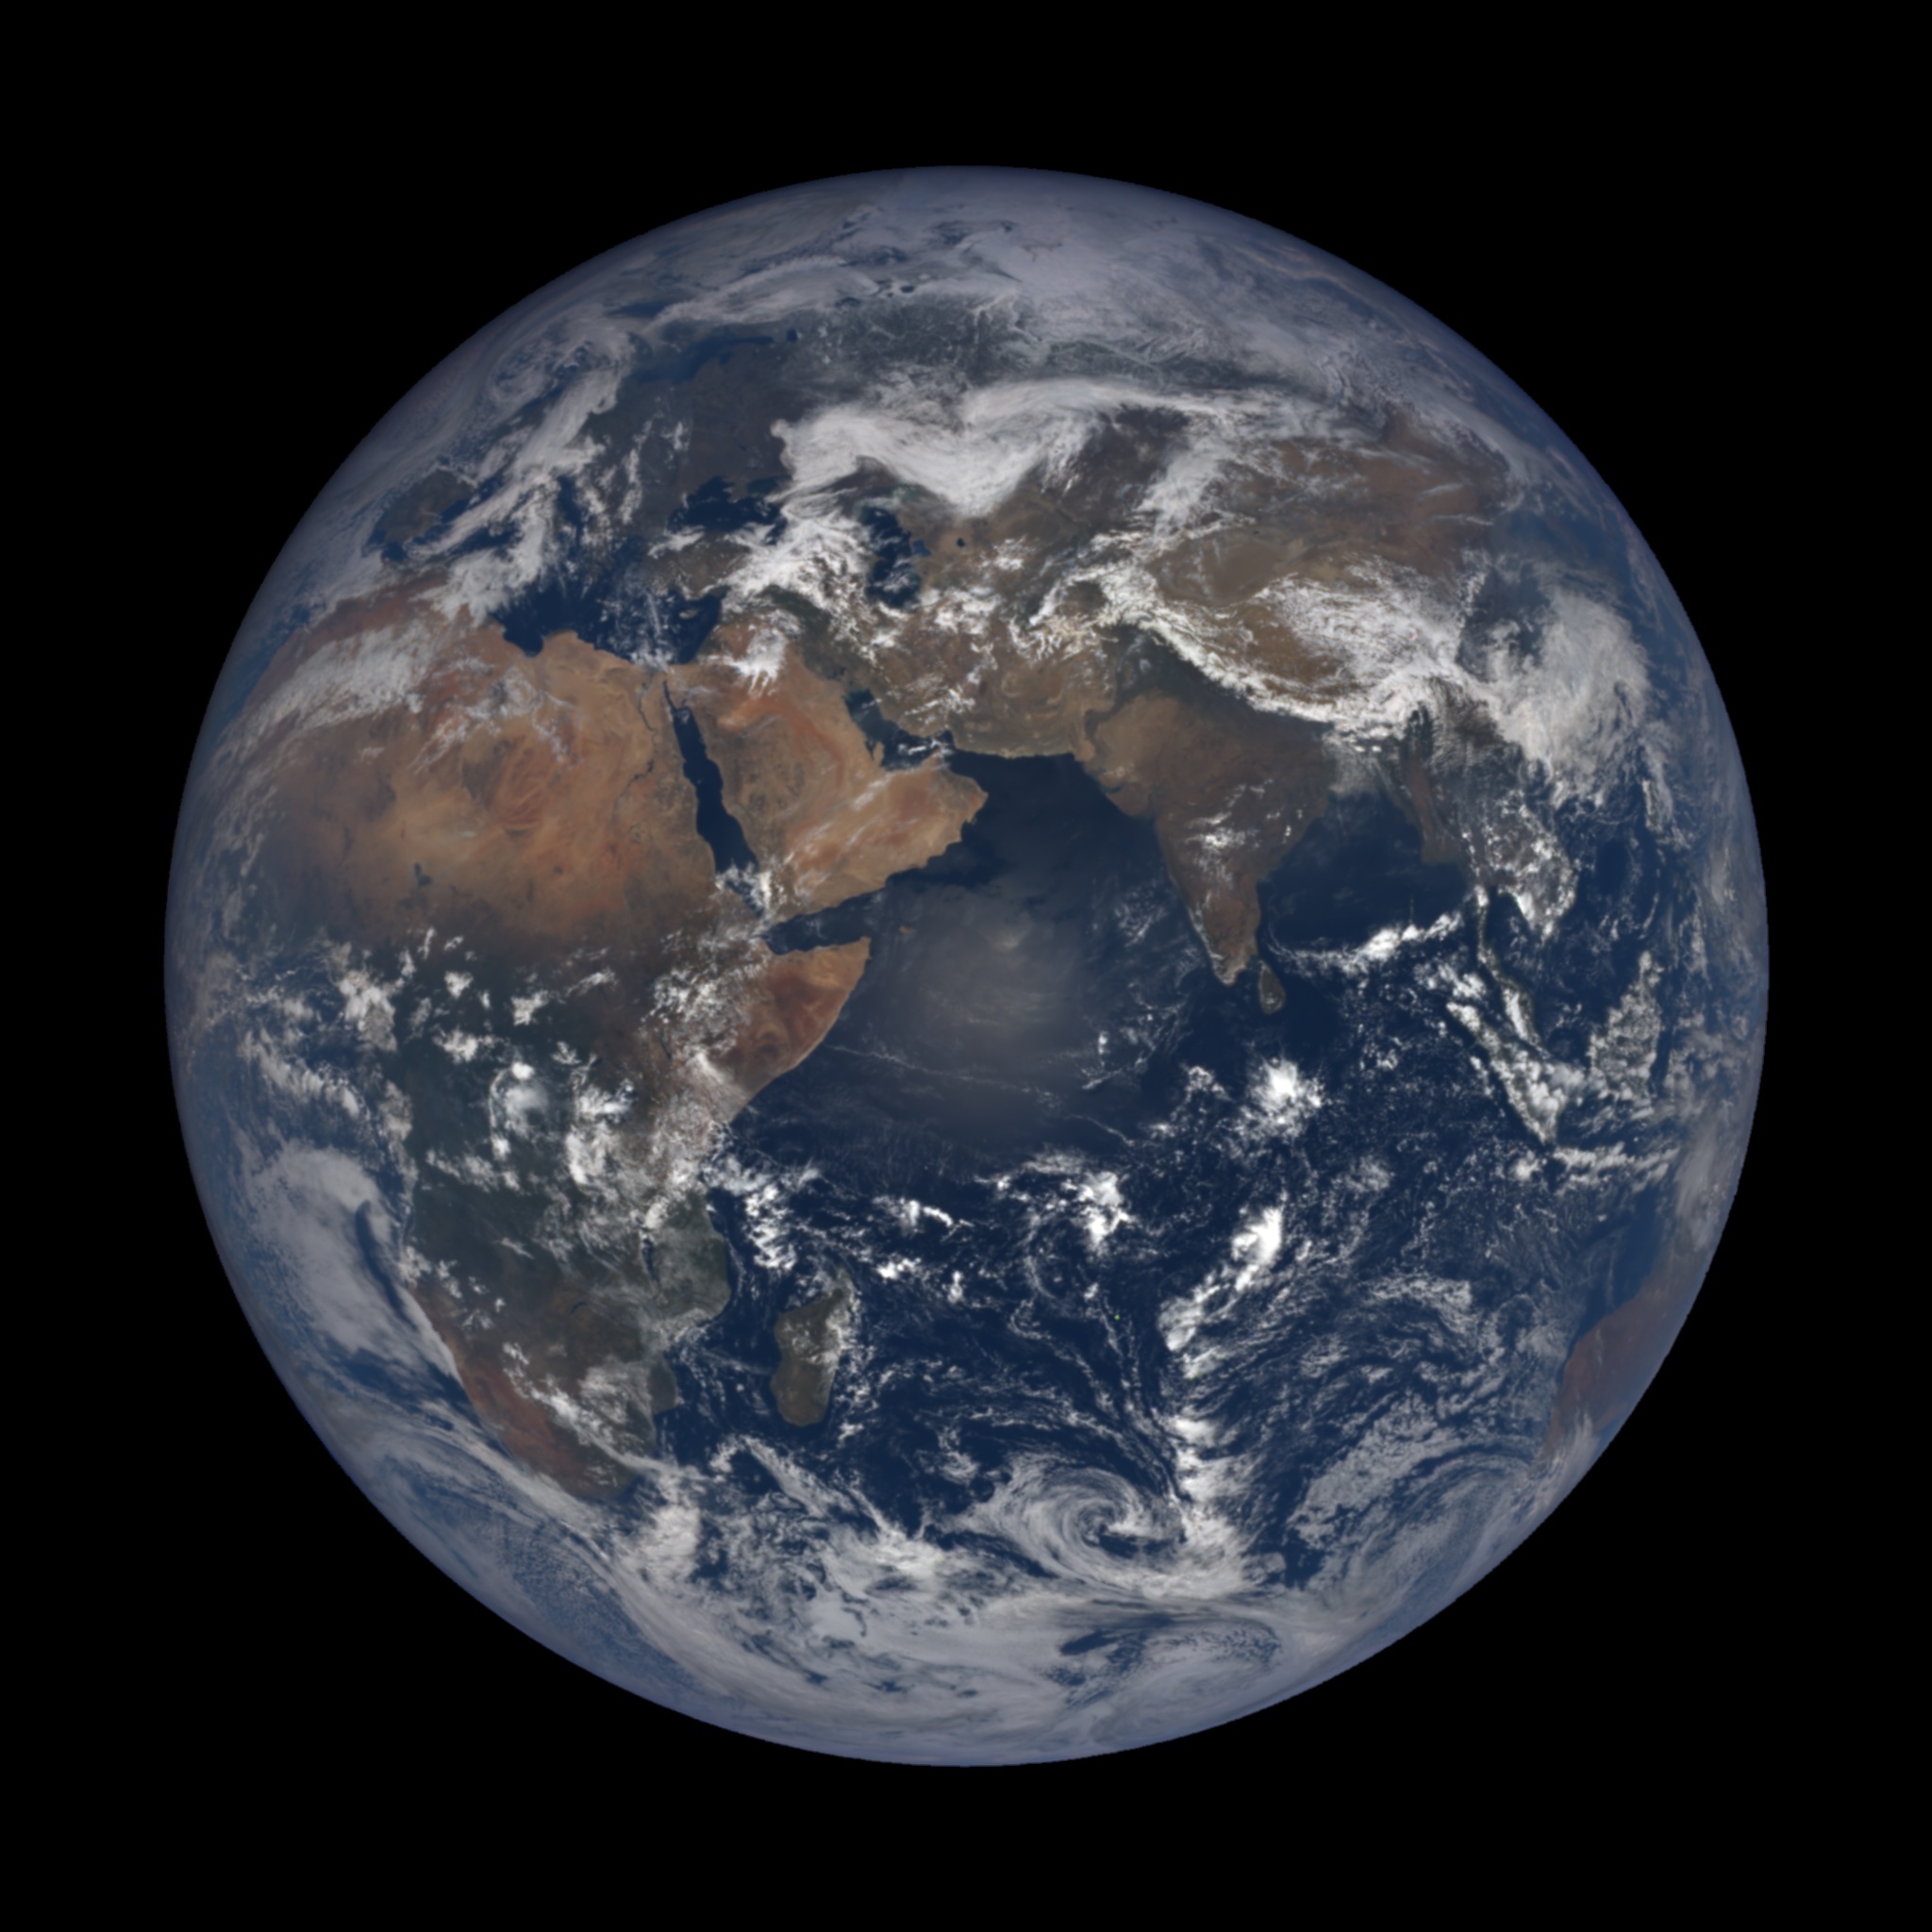
\includegraphics[width=6cm]{images/epic1}
			}
			%		\only<2>{
			%			\textbf{Questions/Input?}
			%			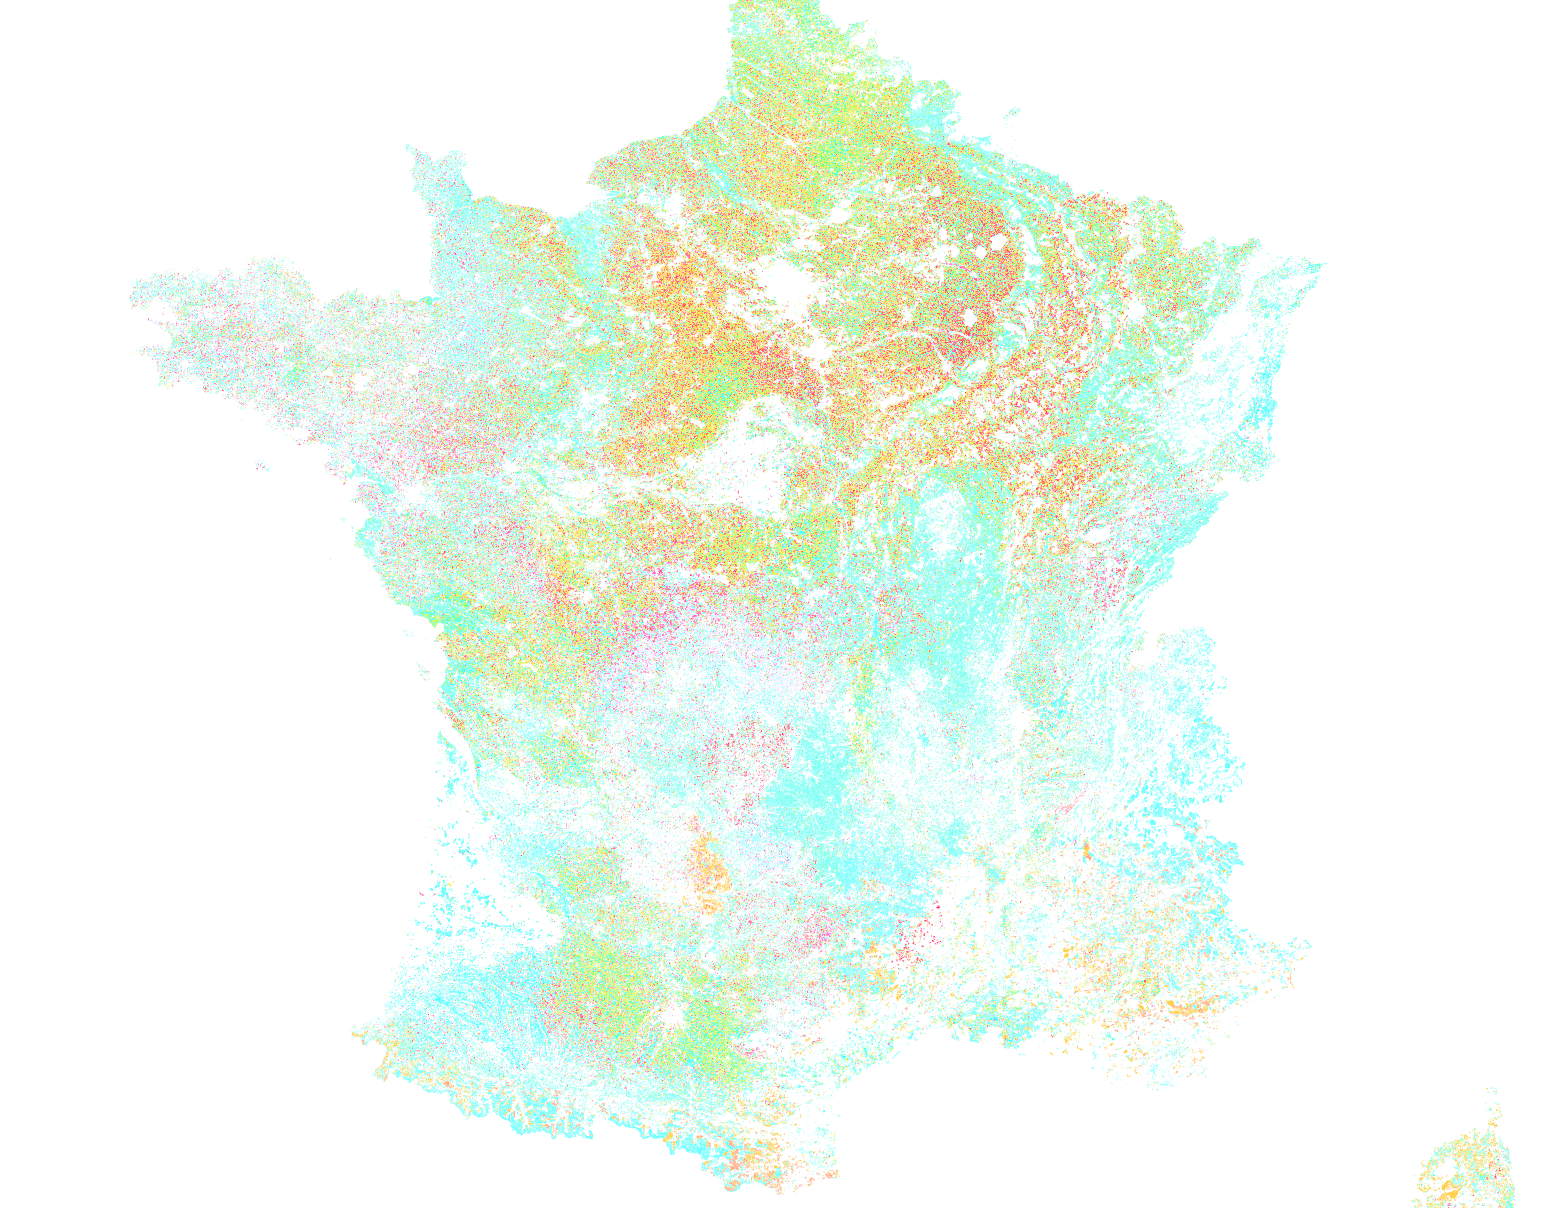
\includegraphics[width=7cm]{images/France_white}
			%		}
			%		\only<3>{
			%			\textbf{Collaborations?}
			%			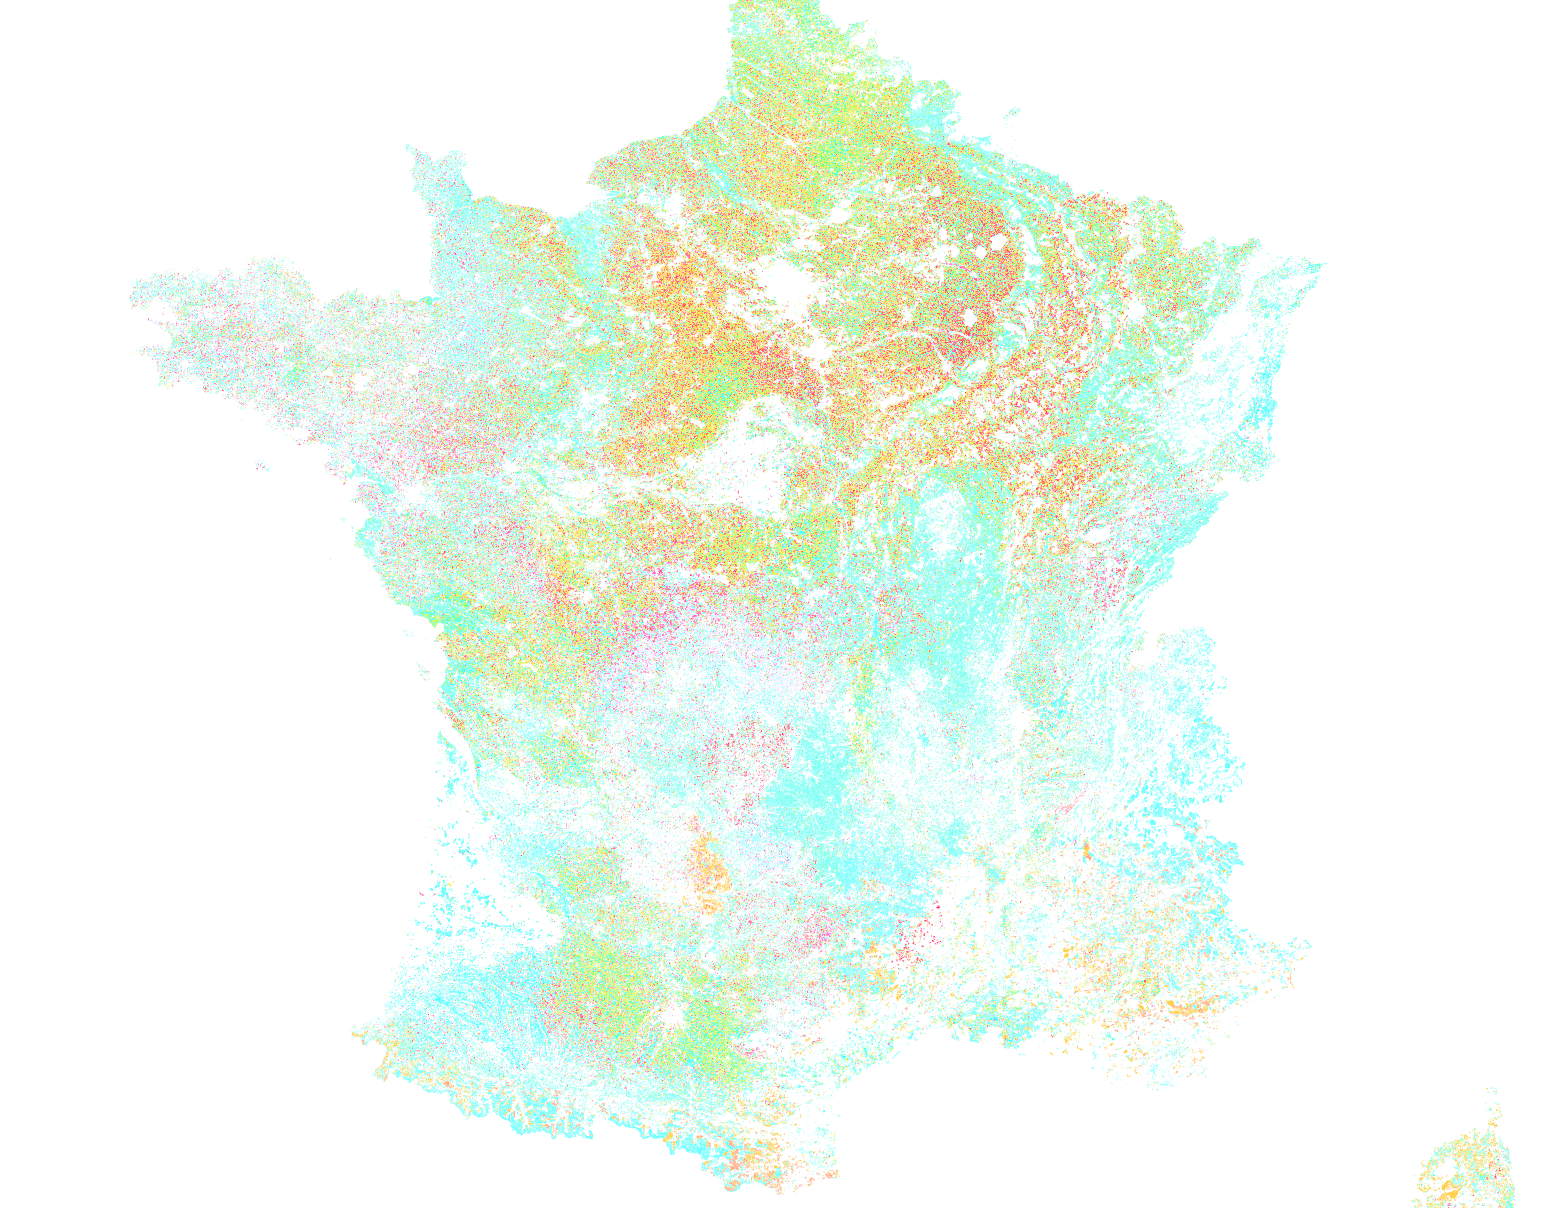
\includegraphics[width=7cm]{images/France_white}
			%		}
			%		
		\end{center}
		
		
		%	\vspace{1em}	
		%	\color{white}
		%	{Twitter}: \textbf{marccoru} | {Github}: \textbf{marccoru} or \textbf{tum-lmf} | 
\includegraphics[height=.9em]{images/TUM-white}~{Chair} \textbf{lmf.bgu.tum.de/vision} \\ 
		%	
		%	\vspace{1em}
		%	
		%	\Large
		%	\url{https://marccoru.github.io/}
		
		\vfill
	\end{frame}
}



{\setbeamercolor{background canvas}{bg=black}
	\begin{frame}[plain]
		\vfill
		\begin{center}
			\Huge\color{tumwhite}
			\only<1>{
				\textbf{backup slides...}
			}
			
		\end{center}
		
		
		\vfill
	\end{frame}
}


{\setbeamercolor{background canvas}{bg=tumbluedark}
	\begin{frame}[plain]
	
	\vfill
	\Huge\color{white}
	\begin{center}
		\begin{columns}
			\column{.5\textwidth}
			\vspace{7em}
			
			\hfill 
			Crop Type Data
			\column{.5\textwidth}
			
			%\includegraphics[width=7cm]{images/fdl}
		\end{columns}
	\end{center}
	
	\vfill
\end{frame}
}


\begin{frame}
\frametitle{Building Large-Scale Crop Type Mapping Datasets}

\begin{columns}

\column{.5\textwidth}

\Large

\begin{description}\setlength\itemsep{1em}
	\item[\color{tumblue}collected] yearly within European \textbf{Common Agricultural Policy} (CAP)
	\item[\color{tumblue}declared] by Farmers at \textbf{crop subsidy} applications
	\item[\color{tumblue}today] slowly made publicly available (on a national basis by French 
\includegraphics[height=.9em]{images/IGN-logo}, Bavarian Stmelf 
\includegraphics[height=.9em]{images/stmelf-logo}, etc.)
	\item[\color{tumblue}in future] further harmonized within \textbf{Europe's INSPIRE} directive
\end{description}

\column{.5\textwidth}
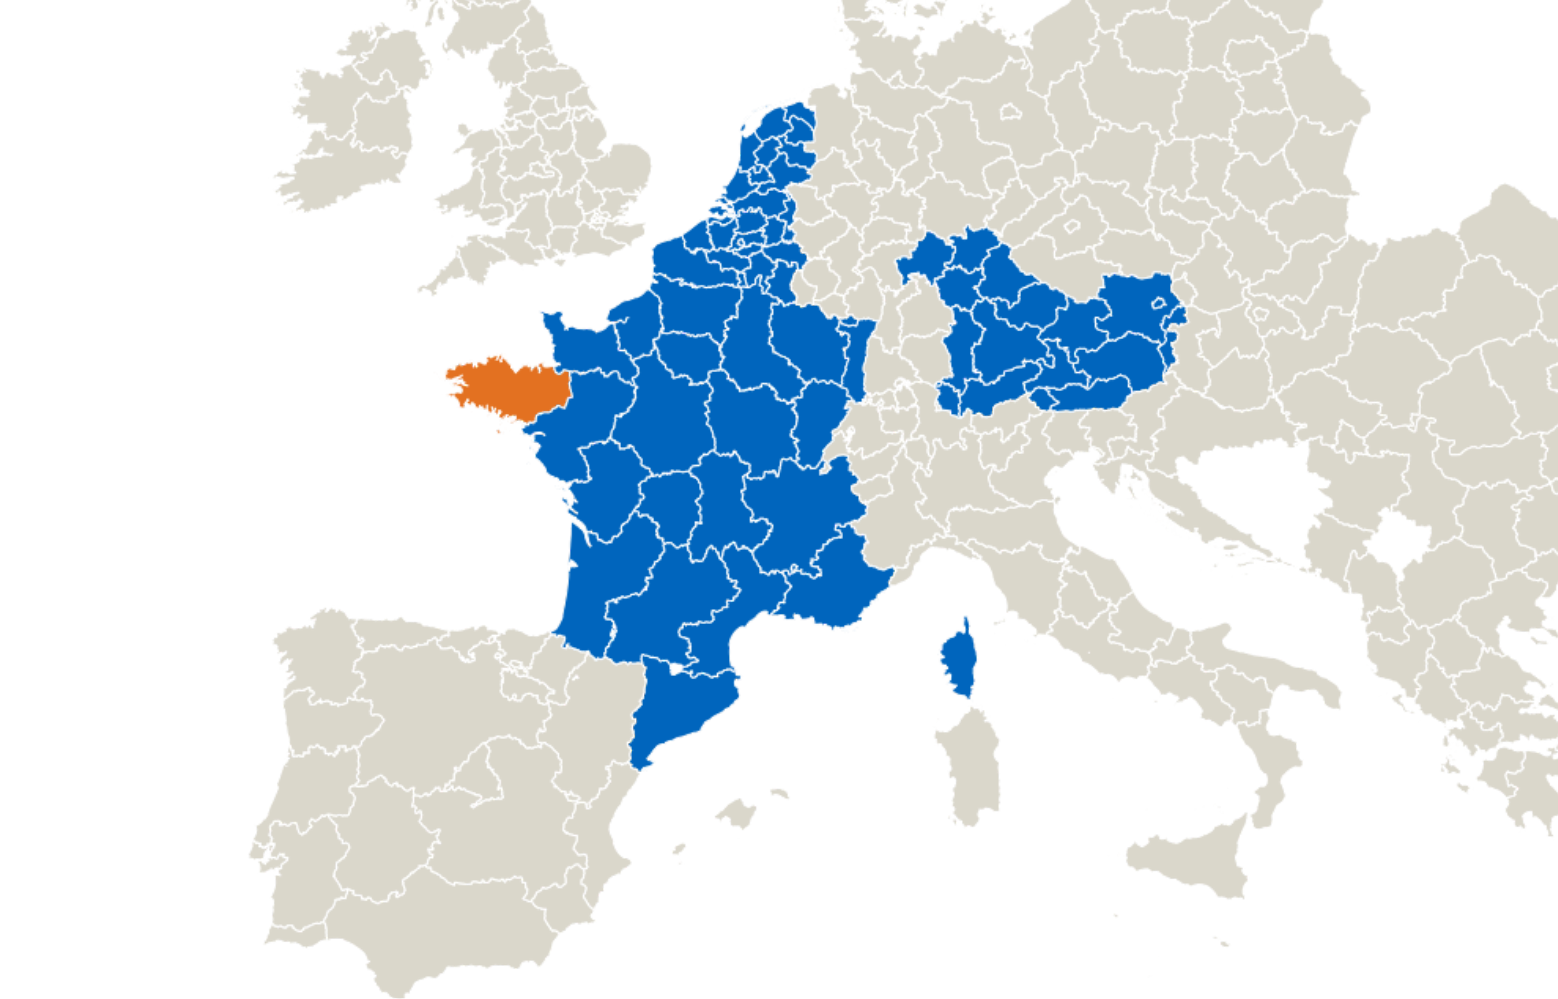
\includegraphics[width=\textwidth]{images/europe_data2}




\end{columns}

\vspace{2em}

\end{frame}


\begin{frame}
\frametitle{Area of Interest for Early Classification}

\begin{columns}
	\column{.4\textwidth}
	\centering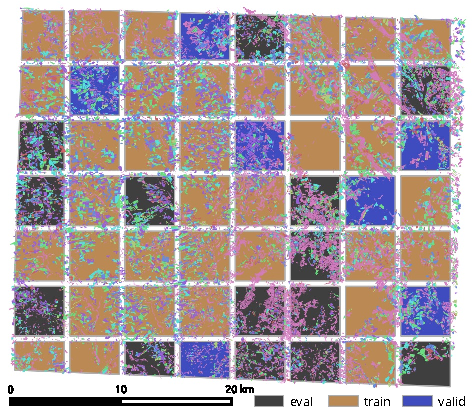
\includegraphics[width=\textwidth]{images/holl.pdf}
	
	The area of interest and partitioning in blocks of 4.5 km for training validation and evaluation
	
	\column{.6\textwidth}
	\tikzsetnextfilename{partition_histograms}
\begin{tikzpicture}
  \centering
  \begin{axis}[
        ybar, axis on top,
        title={},
        height=6cm, width=\textwidth,
        bar width=0.2cm,
        ymajorgrids, tick align=inside,
        major grid style={draw=tumgraylight},
        enlarge y limits={value=.1,upper},
        ymin=0, ymax=60,
        axis x line*=bottom,
        axis y line*=left,
        %ymode=log,
        y axis line style={opacity=0},
        tickwidth=0pt,
        enlarge x limits=true,
        legend style={
            at={(1,0.85)},
            anchor=north east,
            draw=none,
            legend columns=-1,
            rounded corners=0,
            /tikz/every even column/.append style={column sep=0.5cm}
        },
        ylabel={Häufigkeit (\%)},
        symbolic x coords={Wiesen,Sommergerste,Silomais,Winterweizen,Wintergerste,Kleegras,Wintertritikale},
       xtick=data,
       tick label style={rotate=0},
       tick label style={rotate=45,anchor=east},
       ylabel near ticks,
       %nodes near coords={
       % \tiny \pgfmathprintnumber[precision=0]{\pgfplotspointmeta}
       %}
    ]
    \addplot [draw=none, fill=traincolor] coordinates {
(Wiesen, 49.506024096385545)
(Sommergerste, 13.560240963855422)
(Silomais, 9.632530120481928)
(Winterweizen, 8.072289156626505)
(Wintergerste, 8.05421686746988)
(Kleegras, 7.530120481927711)
(Wintertritikale, 3.644578313253012)
  };
   \addplot [draw=none,fill=validcolor] coordinates {
(Wiesen, 49.88550866862938)
(Sommergerste, 13.706247955511941)
(Silomais, 9.846254497873733)
(Winterweizen, 8.897612037945699)
(Wintergerste, 8.27608766764802)
(Kleegras, 6.182531894013739)
(Wintertritikale, 3.205757278377494)
  };
   \addplot [draw=none, fill=evalcolor] coordinates {
(Wiesen, 57.32753103801357)
(Sommergerste, 11.852041469345961)
(Silomais, 8.524254447715347)
(Winterweizen, 6.962754383719442)
(Wintergerste, 6.220401894278766)
(Kleegras, 4.876487904774095)
(Wintertritikale, 4.236528862152822)
  };

    \legend{train,valid,eval}
  \end{axis}
  \end{tikzpicture}
	{Class distribution in the dataset with block-wise separation of train, valid and evaluation partitions.}
	
\end{columns}
\end{frame}



{\setbeamercolor{background canvas}{bg=white}
	\begin{frame}[plain]
	\vfill
	\begin{center}
		\Huge\color{tumblue}
		
		Here, we hand-selected 7 classes from a small region of interest...
		%		
	\end{center}
	
	
\end{frame}
}

\begin{frame}
\frametitle{Large Scale Regional Variations}

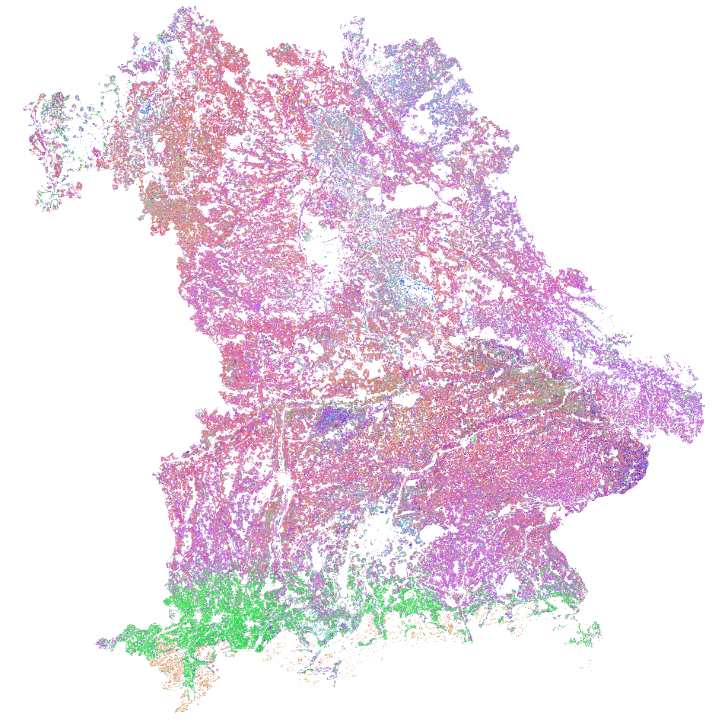
\includegraphics[width=5cm]{images/Bavaria}
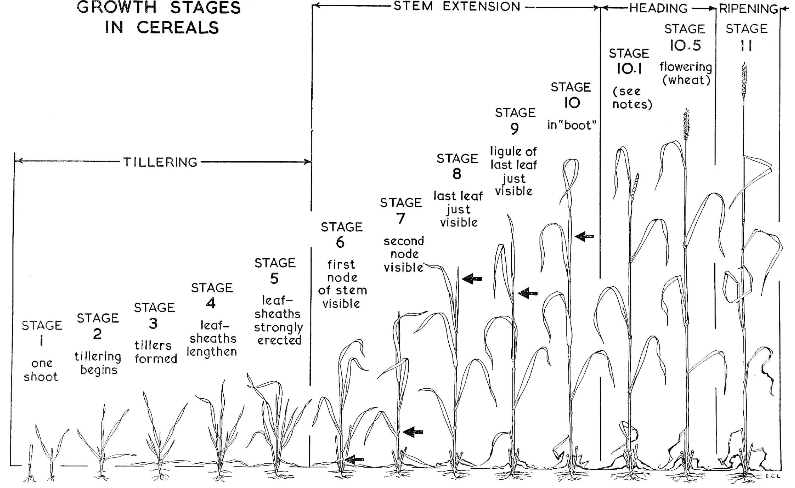
\includegraphics[width=8cm]{images/Large1954_cerial_growth_stages.png}

\raggedleft { \small Large, E. C. (1954). Growth stages in \\ cereals illustration of the Feekes scale. Plant pathology, 3(4), 128-129. }
\end{frame}

\begin{frame}
	\frametitle{Large Scale Regional Variations}
	
	\begin{columns}
		\column{.5\textwidth}
			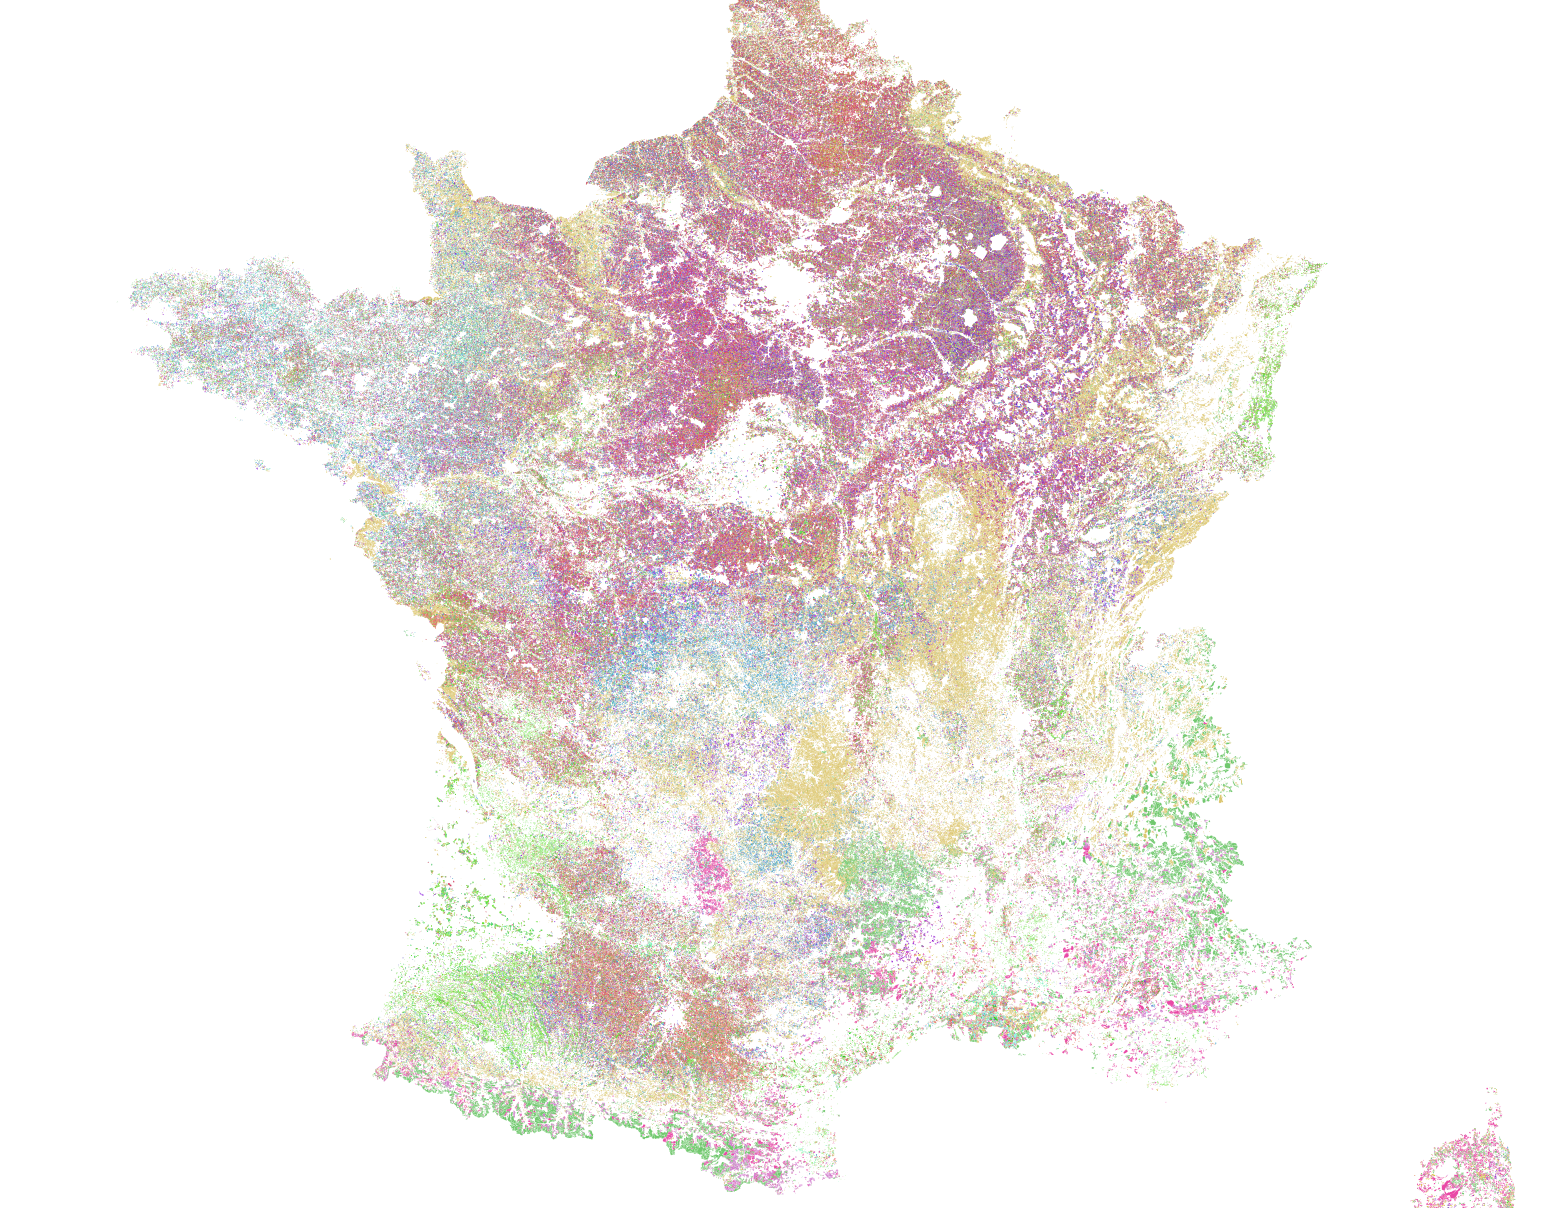
\includegraphics[width=\textwidth]{images/France}
		\column{.5\textwidth}
		\Large
		
		Questions:
			\begin{itemize}
				\item how do we learn models on these inter-regional scales?
				\item the same class label will correspond to different representations in the data.
			\end{itemize}
	\end{columns}
	
\end{frame}

\begin{frame}
	\frametitle{Outlook}
	
	\Large
	
	Goals:
	\begin{itemize}
		\item large-scale domain adaptation between regions of multi-temporal vegetation data
		\item addressing long-tailed class distributions of $>$300 distinct (overlapping) categories with 90\% of data in $<$20 classes
	\end{itemize}

	Short-Term Objective:
	\begin{itemize}
		\item compile a large-scale inter-regional crop type mapping dataset to be able to evaluate these questions
	\end{itemize}
\end{frame}

\begin{frame}
	\frametitle{The Goal}
	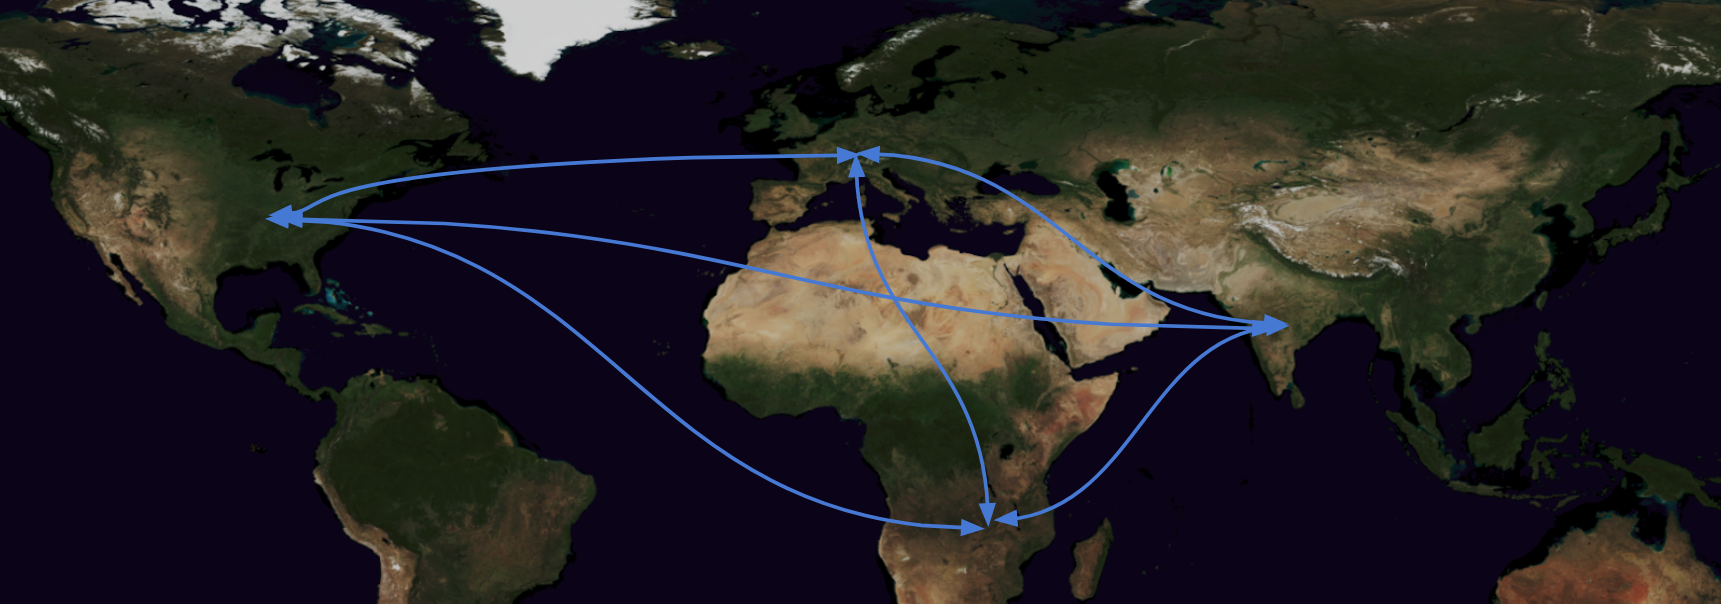
\includegraphics[width=\textwidth]{images/generalization}
\end{frame}

\begin{frame}
\frametitle{BreizhCrops Dataset (ICML Workshop Submission)}

\begin{center}
	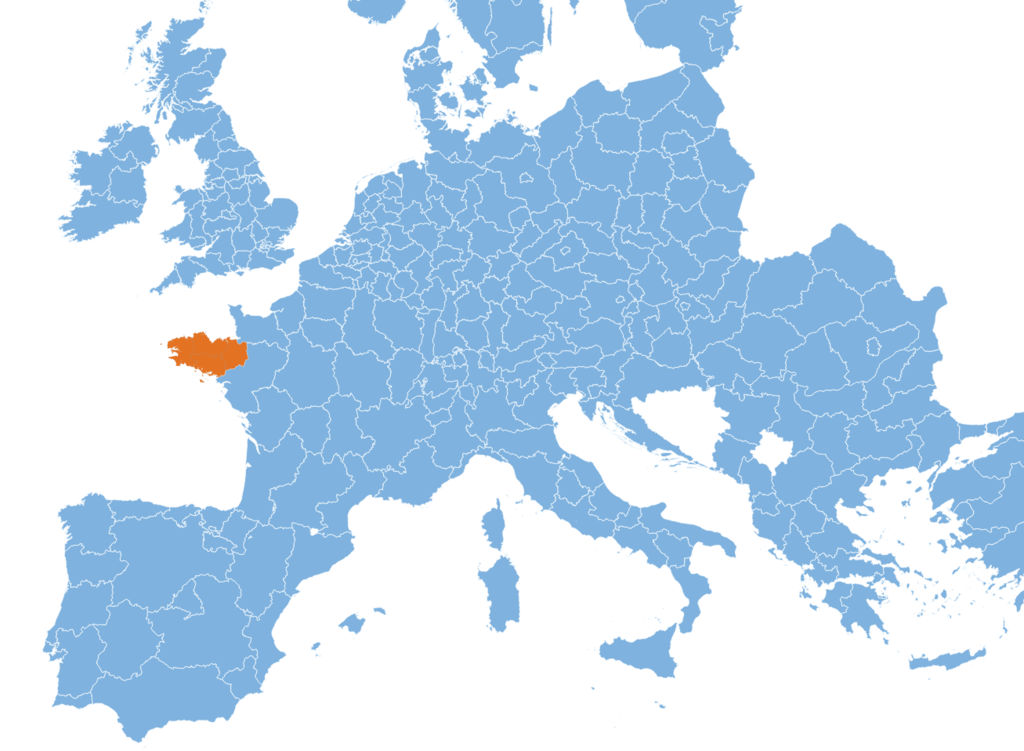
\includegraphics[width=3cm]{images/map/europe}
	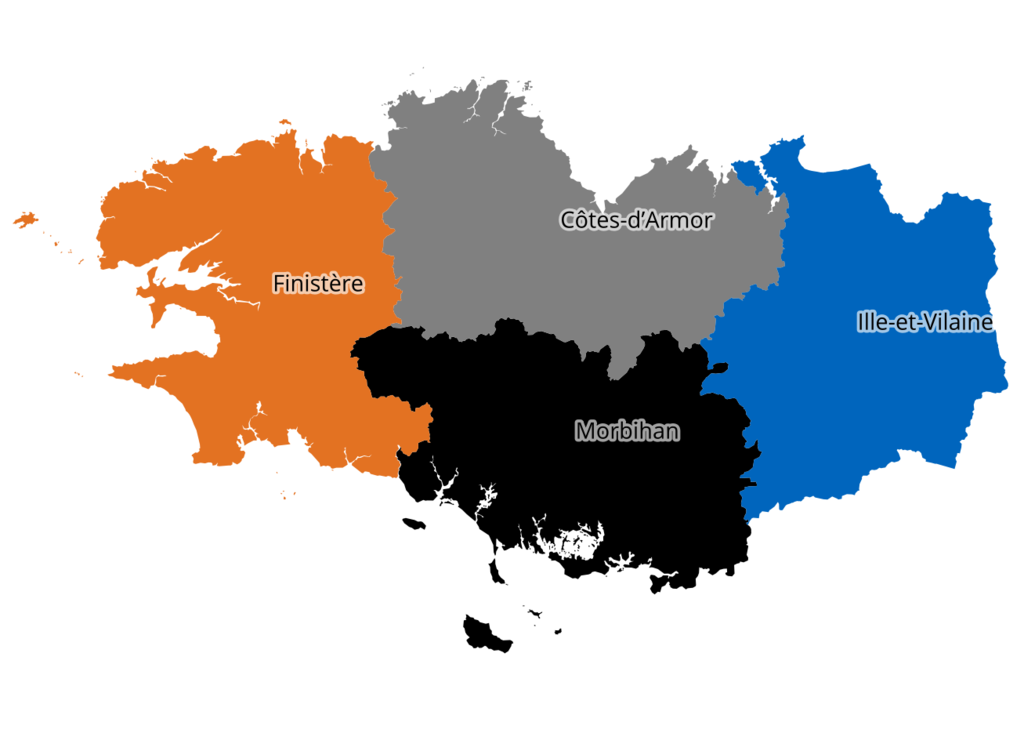
\includegraphics[width=3cm]{images/map/regions}
	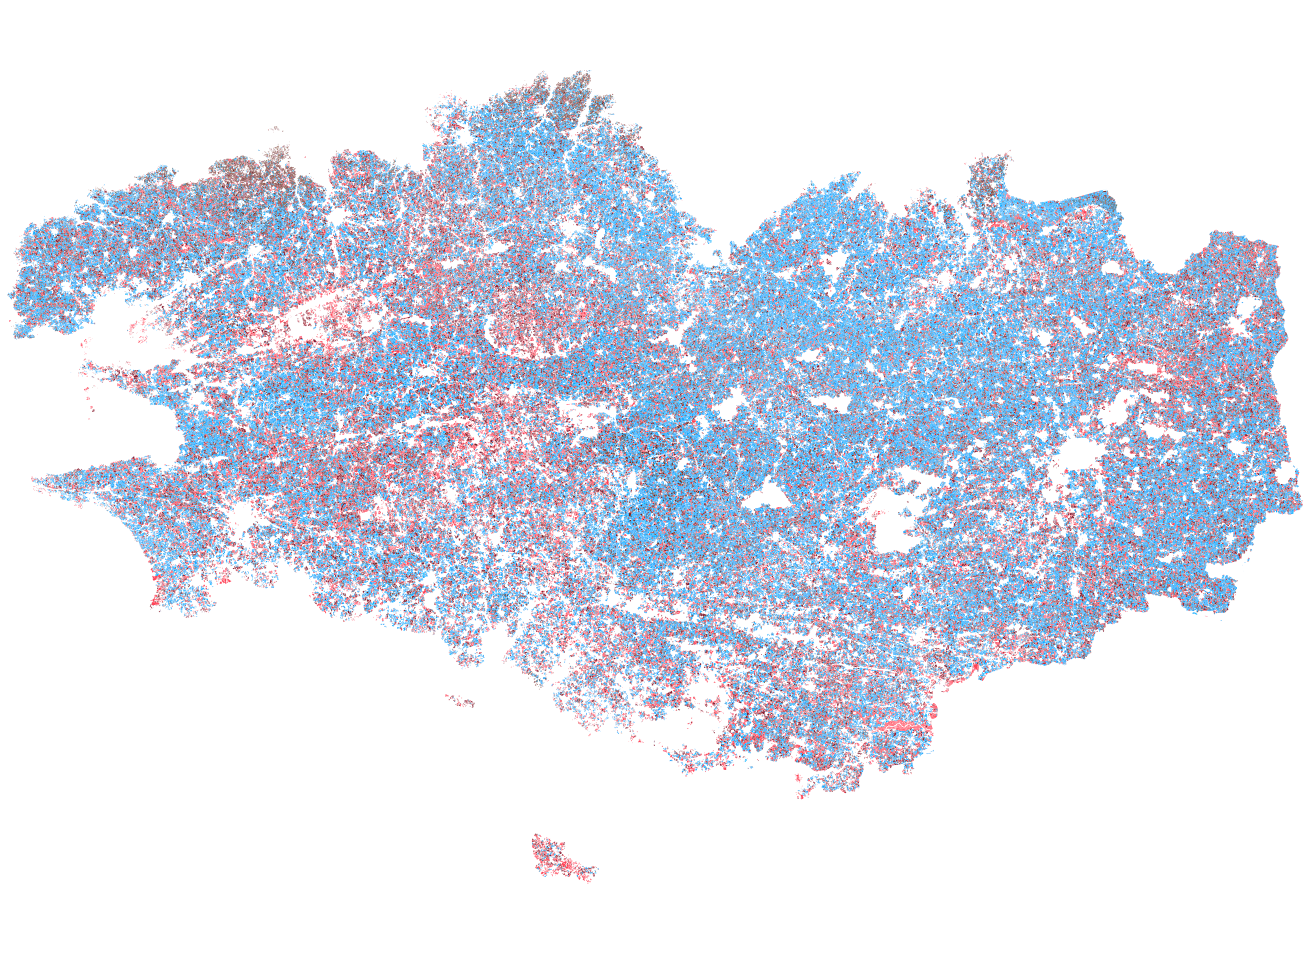
\includegraphics[width=3cm]{images/map/breizh}
	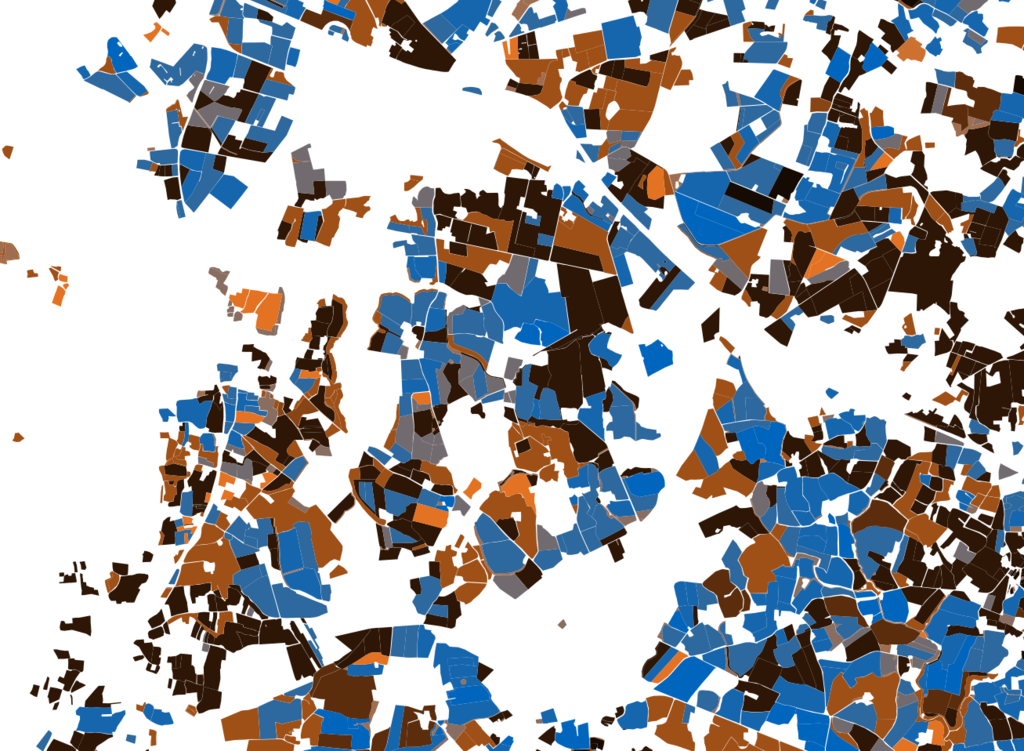
\includegraphics[width=3cm]{images/map/parcels}
\end{center}

%\vspace{1em}

%\tikzsetnextfilename{example}

\newcommand{\dataexample}[1]{
	
	
	


\begin{tikzpicture}
	
	\tikzstyle{annot} = [font=\tiny\sffamily, text=tumblue]
	\tikzstyle{point} = [thin, tumbluelight, shorten >= .25em, shorten <= .25em]
	
	% from /home/marc/projects/EV2019/images/example/tstop.txt
	\def\tstopv{0.6285714285714286}
	\def\class{winter barley}
	
	\begin{groupplot}[
	group style={
		group name=my plots,
		group size=1 by 1,
		columns=1,
		xlabels at=edge bottom,
		xticklabels at=edge bottom,
		vertical sep=1em,
	},
	date coordinates in=x,
	date ZERO=2017-01-01,
	xmin=2017-01-01,
	xmax=2017-12-31,
	ylabel near ticks,
	ylabel style={font=\sffamily\small, rotate=-90},
	width=\textwidth,
	height=3cm,
	axis x line=bottom,
	axis y line=left,
%	enlarge x limits=0.01,
	xtick={2017-01-01,2017-05-01,2017-08-01,2017-12-01},
	xticklabels={January,April,August,December},
	ymajorgrids,
    ymax=10000
	]
	
\nextgroupplot[thin,
%	smooth=1pt,
no marks,  
ylabel={},
draw opacity=.8,
%		tension=0.001,
legend columns=2,
%y tick label style={rotate=90},
legend style={at={(.5,1)},anchor=south, line width=1pt, fill=tumblue!10}
]

\addplot[b1color] table [x=doa, y=B1, col sep=comma, forget plot] {#1};
\addplot[b9color] table [x=doa, y=B9, col sep=comma, forget plot] {#1};
\addplot[b10color] table [x=doa, y=B10, col sep=comma] {#1};

\addplot[b11color] table [x=doa, y=B11, col sep=comma, forget plot] {#1};
\addplot[b12color] table [x=doa, y=B12, col sep=comma] {#1};

\addplot[b5color] table [x=doa, y=B5, col sep=comma, forget plot] {#1};
\addplot[b6color] table [x=doa, y=B6, col sep=comma, forget plot] {#1};
\addplot[b7color] table [x=doa, y=B7, col sep=comma, forget plot] {#1};
\addplot[b8color] table [x=doa, y=B8, col sep=comma, forget plot] {#1};
\addplot[b8Acolor] table [x=doa, y=B8A, col sep=comma] {#1};

\addplot[b2color] table [x=doa, y=B2, col sep=comma, forget plot] {#1};
\addplot[b3color] table [x=doa, y=B3, col sep=comma, forget plot] {#1};
\addplot[b4color] table [x=doa, y=B4, col sep=comma] {#1};
	
%	\draw [red, very thick, ->] ([xshift=5em]plt.north west) -- ([xshift=5em]plt.south west) node [midway, rotate=90, fill=white, yshift=2pt] {faster} ;
%	\node(glab) at (10em,0.5) {ground (signal)};
	
%	\sample{images/example/3685593.csv}
%	
%	\sample{images/example/6053223.csv}
%	\draw[fill=white, draw=none, opacity=.5] (axis cs:\tstopv,0) rectangle (axis cs:1,1.1);
	
%	\node[annot](cllab) at (axis cs:.2,1.3) {clouds (noise)};
%	\draw[point] (cllab) -- (axis cs:.13,.7);
%	\draw[point] (cllab) -- (axis cs:.25,.7);
%	\draw[point] (cllab) -- (axis cs:.53,1);
%	\draw[point] (cllab) -- (axis cs:.45,.85);
%	
%	\node[annot](glab) at (axis cs:.8,1.3) {ground (signal)};
%	\draw[point] (glab) -- (axis cs:.38,.3);
%	\draw[point] (glab) -- (axis cs:.21,.3);
%	\draw[point] (glab) -- (axis cs:.7,.3);
%	
%	\draw (axis cs:\tstopv,0) -- (axis cs:\tstopv,1) node[above]{$\tstop$};
%	
%	
%	
%	\legend{3 atmospheric, 2 short-wave infrared, 5 near infrared, 3 visible bands}
%	
		\end{groupplot}
	
	\end{tikzpicture}
	
}
\begin{columns}
	\column{.5\textwidth}
	
	\textbf{corn grain and silage}
	\dataexample{images/breizhcrops/example/6139251.csv}
	
	\column{.5\textwidth}
	
	\textbf{temporary meadows}
	\dataexample{images/breizhcrops/example/3685593.csv}
	
\end{columns}

%\vspace{1em}


\begin{columns}
	\column{.5\textwidth}
	
	580k samples of Time Series $\M{X}$ and labels $\V{y}$. \Large \url{https://github.com/TUM-LMF/BreizhCrops}
	
	\column{.5\textwidth}
	
	\small\raggedright
	\textsl{
		Rußwurm M., Lefèvre S., and Körner M (2019). \textbf{BreizhCrops: A Satellite Time Series Dataset for Crop Type Identification}. ICML 2019 Time Series Workshop. arXiv:1905.11893
	}
	
\end{columns}

\end{frame}


\begin{frame}
\frametitle{Two Baseline Models}

\Large
Inspired by Models used in NLP, we implemented a \textbf{multi-layer LSTM} and a \textbf{(minified) Transformer encoder}.

\vspace{1em}
\normalsize

%	\begin{table*}[b]
%		\caption{Accuracy metrics for the Multi-layer bidirectional LSTM \cite{hochreiter1997long} and the Transformer-Encoder \cite{Vaswani:transformer}.}
%		\label{tab:accuracies}
%		\centering
\begin{tabular}{lrrrrrrr}
\toprule
baseline & accuracy & $\kappa$ & mean f1 & mean precision  & mean recall \\
\cmidrule(lr){1-1}\cmidrule(lr){2-2}\cmidrule(lr){3-3}\cmidrule(lr){4-4}\cmidrule(lr){5-5}\cmidrule(lr){6-6}\cmidrule(lr){7-7}
Transformer {\small (Vaswani et al., 2017)} & \textbf{0.69}  &  \textbf{0.63} & 0.57 & {0.60} & 0.56 \\
LSTM {\small (Hochreiter and Schmidhuber, 1997)} & 0.68 & 0.62 & \textbf{0.59} & \textbf{0.63} & \textbf{0.58} \\
\bottomrule
\end{tabular}

\vspace{1em}

\Large
\textbf{Takeaway:} 
\begin{itemize}
\item models perform quite similar
\item potential for improvement
\item well-defined classes accurately classified
\item broadly defined classes systematically confused
\end{itemize}
%	\end{table*}

\end{frame}

\begin{frame}
\frametitle{Challenges and Impact}

\Large

\begin{columns}[t]

\column{.5\textwidth}

\visible<1->{
\Large\textbf{Impact}
\vspace{1em}

\begin{description}[itemsep=.5em]
	\item large scale \bluebf{real-world dataset}
	\item effectively \bluebf{unlimited data} (spatially and temporally)
	\item \bluebf{assessing generalization} over large regions
	\item extraction for further \bluebf{vegetation characteristics} in future work (drought indicator, early classification, crop yield)
\end{description}
}

\column{.5\textwidth}

\visible<2->{
\Large\textbf{Challenges}
\vspace{1em}

\begin{description}[itemsep=.5em]
	\item \bluebf{imbalanced} class \bluebf{labels} (>300 raw classes)
	\item classes with \bluebf{similar characteristics}
	\item non-Gaussian noise induced by \bluebf{clouds}
	\item \bluebf{regional} \bluebf{variations} in the class distributions
	\item \bluebf{spatial} \bluebf{autocorrelation}
	\item \bluebf{irregular} temporal \bluebf{sampling} distance
	\item \bluebf{variable} \bluebf{sequence} length
\end{description}
}


\end{columns}
\end{frame}


\newcommand{\good}[1]{\textbf{\color{tumblue}#1}}
\newcommand{\bad}[1]{\textbf{\color{tumorange}#1}}


\newcommand{\confmatgaf}[4]{

\begin{tikzpicture}

  \def\vmax{#3}
  \def\dataindex{#2}
  \def\nclasses{#4}
  
%
%  \pgfplotsset{every axis label/.append style={font=\footnotesize},tick pos=right, ylabel near ticks}
%  
%  \pgfplotsset{
%    axis line style={%
%      opacity=0 
%    }   
%  }

  \begin{groupplot}[
  	group style={
  		group size=2 by 1,
  		xlabels at=edge bottom,
  		ylabels at=edge left,
  		xticklabels at=edge bottom,
  		vertical sep=35pt,
  		group name=seq_len_plot
  	},
  	axis line style={draw=none},
  	title style={yshift=.75em,},
    width=.6\textwidth,
    height=.5\textwidth,
    enlargelimits=false,
    xtick=data,
%     ymin=1,
    xtick distance=1,
    ytick distance=1,
    colormap={example}{%
		color=(tumwhite)
		color=(tumblue)
	},
    ytick=data,
    ytick align=outside,
    xtick align=outside,
%    tick style={draw=none},
    ytick pos = left,  
    tick label style = {font=\small\sansmath\sffamily},
    %xticklabel = {xshift=-0.75cm}
    yticklabel pos=left,
    %yticklabel near ticks,
    xlabel={Prädizierte Klasse},
%    xlabel style={yshift=-2em},
    x label style={at={(axis description cs:0.5,1.1)},anchor=south},
    y label style={at={(axis description cs:0,.5)},anchor=south},
    ylabel={Wahre Klasse},
%     ylabel near ticks,
%    xticklabels={},
  ]
  \nextgroupplot[
%      yticklabels={
%%      	{sugar beet},
%%      	{summer oat},
%%      	{meadow},
%%      	{rape},
%%      	%{vegetable},
%%      	{hop},
%%      	{winter spelt},
%%      	{winter triticale},
%%      	{beans},
%%      	{peas},
%%      	{potato},
%%      	{soybeans},
%%      	{asparagus},
%%      	{winter wheat},
%%      	{winter barley},
%%      	{winter rye},
%%      	{summer barley},
%%      	{maize}
%      },
      xticklabels={
      	\bad{1},2,\bad{3},\bad{4},5,6,7,\good{8},\good{9},10,11,12,13,14,\bad{15},\good{16},\bad{17},18,19,20,21,22
      },
        yticklabels={
  	1,2,3,4,5,6,7,8,9,10,11,12,13,14,15,16,17,18,19,20,21,22
  	},
     %colorbar style={title={\precisionrecall}, xshift=0cm, font=\footnotesize},
     colorbar right,
     colorbar style={
        	title={}, 
        	font=\footnotesize,
        	%at={(0,1)},
        	anchor=north west,
        	width=8pt,
        	ticklabel pos=right,
        	ticklabel style={xshift=2em},
%        	label style={yshift=-1em},
        	rounded corners=1pt
     },
  ]
  
    \addplot[
      matrix plot,
%      draw=tumwhite,
%       nodes near coords=\coordindex,
%       nodes near coords align={center},
%       nodes near coords style={font=\scriptsize},
        shader=faceted,
        faceted color=tumgraylight!20,
%       shader=faceted interp,
      mesh/cols=\nclasses,
      empty line=scanline,
      point meta=explicit,
      point meta min=0,
      point meta max=\vmax,
    ] table[meta index=\dataindex] {#1};
%   \nextgroupplot[
%       title=2017,
%       %colorbar style={title={\precisionrecall}, xshift=0cm, font=\footnotesize},
%       colorbar right,
%       colorbar style={
%       	title={a}, 
%       	font=\footnotesize,
%       	%at={(0,1)},
%       	anchor=north west,
%       	width=8pt,
%       	ticklabel pos=right,
%       	ticklabel style={xshift=1em},
%       	label style={yshift=1em},
%       	rounded corners=1pt
%       },
%       yticklabels={},
%     xticklabels={
%           	{sug.},
%           	{s. oat},
%           	{mead.},
%           	{rape},
%           	%{vegetable},
%           	{hop},
%           	{w. spelt},
%           	{w. trit.},
%           	{beans},
%           	{peas},
%           	{potato},
%           	{soyb.},
%           	{asp.},
%           	{w. wheat},
%           	{w. barley},
%           	{w. rye},
%           	{s. barley},
%           	{maize}
%     },
%       ]
%    
%    \addplot[
%    matrix plot,
%%    draw=tumwhite,
%    ,   
%    %       nodes near coords=\coordindex,
%    %       nodes near coords align={center},
%    %       nodes near coords style={font=\scriptsize},
%    shader=faceted,
%    faceted color=tumgraylight,
%    %       shader=faceted interp,
%    mesh/cols=17,
%    empty line=scanline,
%    point meta=explicit,
%    point meta min=0,
%    point meta max=\vmax,
%    ] table[meta index=\dataindex] {images/confmat/formatted_grucm2017.csv};
    
  \end{groupplot}
\end{tikzpicture}
}
\begin{frame}
\frametitle{Verwechslungen}

\centering

\vspace{-2em}

\confmatgaf{images/data/TUM_ALL_rnn/npy/confmat_flat.csv}{3}{1}{22}
\end{frame}




\begin{frame}
\frametitle{83 Finale Kategorien}

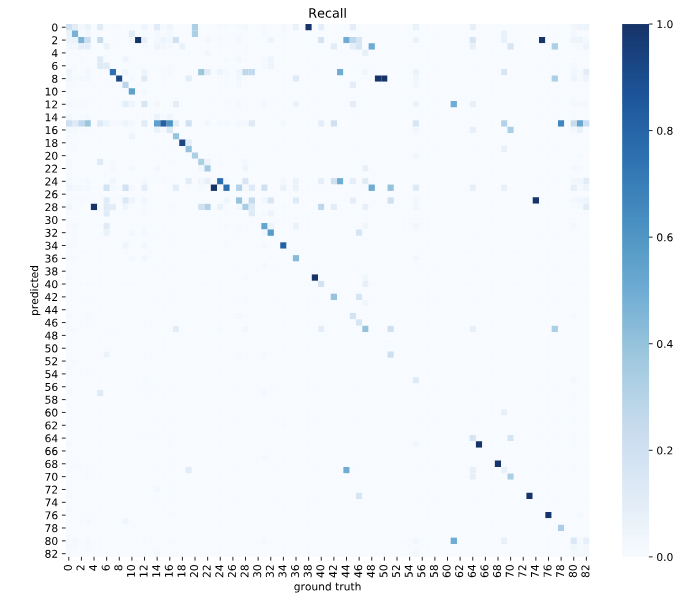
\includegraphics[width=.49\textwidth]{images/83_confmat1}
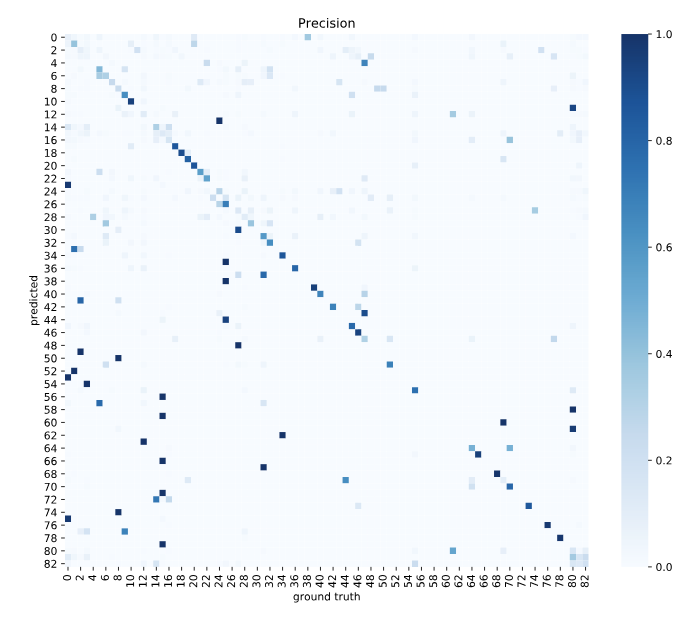
\includegraphics[width=.49\textwidth]{images/83_confmat2}

\end{frame}










\begin{frame}


\begin{table}
	\caption{Varying the weighting factor $\alpha$ for the two loss formulations \emph{early reward} (\cref{sec:earlynessreward}) and \emph{lateness penalty} (\cref{sec:twophasecrossentropy}).}
	\label{tab:alpha}
	
	\setlength{\belowcaptionskip}{0pt}
	
	\begin{subtable}{.5\textwidth}
		\scriptsize
		\hspace{0em}\begin{tabular}{lcccccc}
			\toprule
			\textbf{$\alpha$} & accuracy & $\meantstop$ & precision & recall & $f_1$ & $\kappa$ \\
			\cmidrule(lr){0-0}\cmidrule(lr){1-1}\cmidrule(lr){2-2}\cmidrule(lr){3-3}\cmidrule(lr){4-4}\cmidrule(lr){5-5}\cmidrule(lr){6-6}\cmidrule(lr){7-7}
			.0 & .24 $\pm$ .29 & .00 $\pm$ .00 & .04 $\pm$ .04 & .15 $\pm$ .00 & .05 $\pm$ .05 & .00 $\pm$ .00 \\
			.2 & .15 $\pm$ .08 & .00 $\pm$ .00 & .10 $\pm$ .05 & .15 $\pm$ .01 & .08 $\pm$ .03 & .01 $\pm$ .01 \\
			.4 & .79 $\pm$ .05 & .39 $\pm$ .03 & .67 $\pm$ .05 & .71 $\pm$ .04 & .68 $\pm$ .04 & .69 $\pm$ .06 \\
			.6 & .83 $\pm$ .03 & .59 $\pm$ .17 & .71 $\pm$ .03 & .74 $\pm$ .02 & .72 $\pm$ .02 & .74 $\pm$ .04 \\
			.8 & .86 $\pm$ .01 & .86 $\pm$ .12 & .74 $\pm$ .01 & .76 $\pm$ .02 & .75 $\pm$ .02 & .79 $\pm$ .01 \\
			1.0 & .86 $\pm$ .01 & 1.00 $\pm$ .00 & .75 $\pm$ .02 & .76 $\pm$ .02 & .75 $\pm$ .02 & .79 $\pm$ .02 \\
			\bottomrule
		\end{tabular}
		\caption{two-phase \emph{lateness penalty} loss formulation}
		\label{tab:alpha:xentropy}
	\end{subtable}
	\begin{subtable}{.5\textwidth}
		\scriptsize
		\hspace{0em}\begin{tabular}{lcccccc}
			\toprule\small
			\textbf{$\alpha$} & accuracy & $\meantstop$  & precision & recall & $f_1$ & $\kappa$ \\
			\cmidrule(lr){0-0}\cmidrule(lr){1-1}\cmidrule(lr){2-2}\cmidrule(lr){3-3}\cmidrule(lr){4-4}\cmidrule(lr){5-5}\cmidrule(lr){6-6}\cmidrule(lr){7-7}
			.0 & .25 $\pm$ .22 & .10 $\pm$ .17 & .19 $\pm$ .20 & .25 $\pm$ .17 & .16 $\pm$ .20 & .12 $\pm$ .19 \\
			.2 & .81 $\pm$ .03 & .40 $\pm$ .02 & .70 $\pm$ .01 & .74 $\pm$ .01 & .71 $\pm$ .01 & .71 $\pm$ .04 \\
			.4 & .80 $\pm$ .09 & .47 $\pm$ .03 & .71 $\pm$ .02 & .74 $\pm$ .01 & .71 $\pm$ .02 & .71 $\pm$ .10 \\
			.6 & .85 $\pm$ .02 & .88 $\pm$ .07 & .73 $\pm$ .04 & .74 $\pm$ .03 & .73 $\pm$ .03 & .77 $\pm$ .03 \\
			.8 & .84 $\pm$ .01 & .93 $\pm$ .05 & .72 $\pm$ .02 & .75 $\pm$ .01 & .73 $\pm$ .02 & .76 $\pm$ .02 \\
			1.0 & .83 $\pm$ .03 & 1.00 $\pm$ .00 & .72 $\pm$ .03 & .75 $\pm$ .01 & .72 $\pm$ .03 & .75 $\pm$ .04 \\
			\bottomrule
		\end{tabular}
		\caption{one phase \emph{early-reward} formulation}
		\label{tab:alpha:earlyreward}
	\end{subtable}
	
\end{table}

\end{frame}


\begin{frame}


\begin{table}
	\caption{Quantitative analysis of the $\ptoffset$ parameter on different trade-off factors between $\alpha$ earliness and accuracy. The illustrated figures show the mean and standard deviation of three runs with same parameters, but different initial random initialization.}
	\label{tab:epsilon:quantitative}
	\setlength{\belowcaptionskip}{0pt}
	
	\begin{subtable}{.5\textwidth}
		\scriptsize
		%\begin{tabular}{lcccccc}
		%	\toprule
		%	\textbf{$\ptoffset$} & accuracy & earliness & $f_1$ & precision & recall & $\kappa$ \\
		%	\cmidrule(lr){0-0}\cmidrule(lr){1-1}\cmidrule(lr){2-2}\cmidrule(lr){3-3}\cmidrule(lr){4-4}\cmidrule(lr){5-5}\cmidrule(lr){6-6}\cmidrule(lr){7-7}
		%0 & .05 $\pm$ .00 & .00 $\pm$ .00 & .01 $\pm$ .00 & .01 $\pm$ .00 & .14 $\pm$ .00 & .00 $\pm$ .00 \\
		%1 & .41 $\pm$ .26 & .08 $\pm$ .13 & .12 $\pm$ .09 & .11 $\pm$ .09 & .19 $\pm$ .07 & .11 $\pm$ .17 \\
		%10 & .25 $\pm$ .22 & .10 $\pm$ .17 & .16 $\pm$ .20 & .19 $\pm$ .20 & .25 $\pm$ .17 & .12 $\pm$ .19 \\
		%	\bottomrule
		%\end{tabular}
		%\caption{\emph{$\alpha=0$}}
		%\label{tab:epsilon:a0}
		\hspace{-1em}\begin{tabular}{lcccccc}
			\toprule
			\textbf{$\ptoffset$} & accuracy & $\meantstop$  & $f_1$ & precision & recall & $\kappa$ \\
			\cmidrule(lr){0-0}\cmidrule(lr){1-1}\cmidrule(lr){2-2}\cmidrule(lr){3-3}\cmidrule(lr){4-4}\cmidrule(lr){5-5}\cmidrule(lr){6-6}\cmidrule(lr){7-7}
			0 & .10 $\pm$ .02 & .02 $\pm$ .00 & .07 $\pm$ .01 & .13 $\pm$ .06 & .17 $\pm$ .00 & .02 $\pm$ .00 \\
			1 & .75 $\pm$ .09 & .44 $\pm$ .06 & .65 $\pm$ .05 & .64 $\pm$ .03 & .69 $\pm$ .03 & .64 $\pm$ .10 \\
			10 & .81 $\pm$ .03 & .40 $\pm$ .02 & .71 $\pm$ .01 & .70 $\pm$ .01 & .74 $\pm$ .01 & .71 $\pm$ .04 \\
			\bottomrule
		\end{tabular}
		\caption{\emph{$\alpha=0.2$}}
		\label{tab:epsilon:a02}
	\end{subtable}
	\begin{subtable}{.5\textwidth}
		\scriptsize
		\hspace{-1em}\begin{tabular}{lcccccc}
			\toprule
			\textbf{$\ptoffset$} & accuracy & $\meantstop$  & $f_1$ & precision & recall & $\kappa$ \\
			\cmidrule(lr){0-0}\cmidrule(lr){1-1}\cmidrule(lr){2-2}\cmidrule(lr){3-3}\cmidrule(lr){4-4}\cmidrule(lr){5-5}\cmidrule(lr){6-6}\cmidrule(lr){7-7}
			0 & .21 $\pm$ .20 & .02 $\pm$ .00 & .09 $\pm$ .04 & .18 $\pm$ .03 & .16 $\pm$ .01 & .04 $\pm$ .03 \\
			1 & .80 $\pm$ .02 & .50 $\pm$ .05 & .68 $\pm$ .05 & .67 $\pm$ .05 & .70 $\pm$ .07 & .70 $\pm$ .03 \\
			10 & .80 $\pm$ .09 & .47 $\pm$ .03 & .71 $\pm$ .02 & .71 $\pm$ .02 & .74 $\pm$ .01 & .71 $\pm$ .10 \\
			\bottomrule
		\end{tabular}
		\caption{\emph{$\alpha=0.4$}}
		\label{tab:epsilon:a04}
	\end{subtable}
	\begin{subtable}{.5\textwidth}
		\scriptsize
		\hspace{-1em}\begin{tabular}{lcccccc}
			\toprule
			\textbf{$\ptoffset$} & accuracy & $\meantstop$  & $f_1$ & precision & recall & $\kappa$ \\
			\cmidrule(lr){0-0}\cmidrule(lr){1-1}\cmidrule(lr){2-2}\cmidrule(lr){3-3}\cmidrule(lr){4-4}\cmidrule(lr){5-5}\cmidrule(lr){6-6}\cmidrule(lr){7-7}
			0 & .13 $\pm$ .04 & .02 $\pm$ .00 & .08 $\pm$ .01 & .16 $\pm$ .01 & .16 $\pm$ .01 & .02 $\pm$ .01 \\
			1 & .80 $\pm$ .05 & .85 $\pm$ .14 & .71 $\pm$ .02 & .70 $\pm$ .02 & .74 $\pm$ .01 & .70 $\pm$ .06 \\
			10 & .85 $\pm$ .02 & .88 $\pm$ .07 & .73 $\pm$ .03 & .73 $\pm$ .04 & .74 $\pm$ .03 & .77 $\pm$ .03 \\
			\bottomrule
		\end{tabular}
		\caption{\emph{$\alpha=0.6$}}
		\label{tab:epsilon:a06}
	\end{subtable}
	\begin{subtable}{.5\textwidth}
		\scriptsize
		\hspace{-1em}\begin{tabular}{lcccccc}
			\toprule
			\textbf{$\ptoffset$} & accuracy & $\meantstop$  & $f_1$ & precision & recall & $\kappa$ \\
			\cmidrule(lr){0-0}\cmidrule(lr){1-1}\cmidrule(lr){2-2}\cmidrule(lr){3-3}\cmidrule(lr){4-4}\cmidrule(lr){5-5}\cmidrule(lr){6-6}\cmidrule(lr){7-7}
			0 & .11 $\pm$ .03 & .03 $\pm$ .01 & .08 $\pm$ .02 & .15 $\pm$ .02 & .17 $\pm$ .01 & .02 $\pm$ .01 \\
			1 & .84 $\pm$ .03 & .98 $\pm$ .03 & .73 $\pm$ .03 & .72 $\pm$ .04 & .75 $\pm$ .02 & .76 $\pm$ .04 \\
			10 & .84 $\pm$ .01 & .93 $\pm$ .05 & .73 $\pm$ .02 & .72 $\pm$ .02 & .75 $\pm$ .01 & .76 $\pm$ .02 \\
			\bottomrule
		\end{tabular}
		\caption{\emph{$\alpha=0.8$}}
		\label{tab:epsilon:a08}
	\end{subtable}
	%\begin{subtable}{.5\textwidth}
	%	\scriptsize
	%	\hspace{-1em}\begin{tabular}{lcccccc}
	%		\toprule
	%		\textbf{$\ptoffset$} & accuracy & $\meantstop$ & $f_1$ & precision & recall & $\kappa$ \\
	%		\cmidrule(lr){0-0}\cmidrule(lr){1-1}\cmidrule(lr){2-2}\cmidrule(lr){3-3}\cmidrule(lr){4-4}\cmidrule(lr){5-5}\cmidrule(lr){6-6}\cmidrule(lr){7-7}
	%0 & .39 $\pm$ .30 & 1.00 $\pm$ .00 & .14 $\pm$ .15 & .13 $\pm$ .15 & .23 $\pm$ .14 & .12 $\pm$ .21 \\
	%1 & .74 $\pm$ .14 & 1.00 $\pm$ .00 & .51 $\pm$ .36 & .50 $\pm$ .36 & .55 $\pm$ .35 & .49 $\pm$ .42 \\
	%10 & .83 $\pm$ .03 & 1.00 $\pm$ .00 & .72 $\pm$ .03 & .72 $\pm$ .03 & .75 $\pm$ .01 & .75 $\pm$ .04 \\
	%		\bottomrule
	%	\end{tabular}
	%	\caption{\emph{$\alpha=1.0$}}
	%	\label{tab:epsilon:a1}
	%\end{subtable}
	
\end{table}

\end{frame}


%\begin{frame}
%Epsilon
%\end{frame}

\begin{frame}

\newcommand{\figepsilonzero}{
\def\datapath{images/logs/data/epsilon0}
\tikzsetnextfilename{epsilonexperiment}
\begin{tikzpicture}
	\begin{groupplot}[
	group style = {
		group size = 1 by 3,
		x descriptions at=edge bottom,
		vertical sep=.5em},
	no markers,
	height=2.8cm,
%	legend style={at={(0.03,0.5)},anchor=west},
	legend style={at={(1,1)},anchor=south east},
	width=\linewidth,
	xlabel=epochs,
	legend columns=3, 
	ytick={0,0.5,1},
	yticklabels={0,0.5,1},
	ylabel=$\meantstop$
 	]
%	\nextgroupplot[legend columns=1, ylabel=loss]
%
%	\addplot[epsilon10color] table [x=epoch, y=loss_classification, col sep=comma] {images/logs/data/epsilon10/log_earliness_test.csv};
%	\addplot[epsilon10color] table [x=epoch, y=earliness_reward, col sep=comma] {images/logs/data/epsilon10/log_earliness_test.csv};
%	
%	\addplot[epsilon1color] table [x=epoch, y=loss_classification, col sep=comma] {images/logs/data/epsilon1/log_earliness_test.csv};
%	\addplot[epsilon1color] table [x=epoch, y=earliness_reward, col sep=comma] {images/logs/data/epsilon1/log_earliness_test.csv};
%	
%	\addplot[epsilon0color] table [x=epoch, y=loss_classification, col sep=comma] {images/logs/data/epsilon0/log_earliness_test.csv};
%	\addplot[epsilon0color] table [x=epoch, y=earliness_reward, col sep=comma] {images/logs/data/epsilon0/log_earliness_test.csv};
%	
%	
%%	\legend{total loss (eval), classification loss (eval), earliness reward (eval)}
%%	
%	\legend{$\mathcal{L}_\text{c} - \mathcal{R}_\text{e}$, $\mathcal{L}_\text{c}$, $\mathcal{R}_\text{e}$}
%	
	
	
	\nextgroupplot[]
	\legend{$\epsilon = 10$,$\epsilon = 1$,$\epsilon = 0$,}
	
	\addplot[epsilon10color] table [x=epoch, y=earliness, col sep=comma] {images/logs/data/epsilon10_r0/log_earliness_test.csv};
	\addplot[epsilon1color] table [x=epoch, y=earliness, col sep=comma] {images/logs/data/epsilon1_r0/log_earliness_test.csv};
	\addplot[epsilon0color] table [x=epoch, y=earliness, col sep=comma] {images/logs/data/epsilon0_r0/log_earliness_test.csv};
	
	\nextgroupplot[]
	
	\addplot[epsilon10color] table [x=epoch, y=earliness, col sep=comma] {images/logs/data/epsilon10_r1/log_earliness_test.csv};
	\addplot[epsilon1color] table [x=epoch, y=earliness, col sep=comma] {images/logs/data/epsilon1_r1/log_earliness_test.csv};
	\addplot[epsilon0color] table [x=epoch, y=earliness, col sep=comma] {images/logs/data/epsilon0_r1/log_earliness_test.csv};
	
	
	\nextgroupplot[]
	
	\addplot[epsilon10color] table [x=epoch, y=earliness, col sep=comma] {images/logs/data/epsilon10_r2/log_earliness_test.csv};
	\addplot[epsilon1color] table [x=epoch, y=earliness, col sep=comma] {images/logs/data/epsilon1_r2/log_earliness_test.csv};
	\addplot[epsilon0color] table [x=epoch, y=earliness, col sep=comma] {images/logs/data/epsilon0_r2/log_earliness_test.csv};
	
	
	
	
	\end{groupplot}
\end{tikzpicture}

}
\figepsilonzero
{The three runs with different random initialization per $\ptoffset$ offset and $\alpha=0.4$ of \cref{tab:epsilon:a04}.
The $\ptoffset>0$ offset factor allows the models to recover from a too early classification, as is visible in the top two plots.}

\end{frame}





\end{document}



